\documentclass[11pt, a4paper, oneside, openany]{book}
\usepackage{textcomp}
\usepackage[utf8]{inputenc}
%\usepackage[T1]{fontenc} For some reason this causes all fonts to be bitmap.
\usepackage{makeidx}
\usepackage[italian, french, english]{babel}
\usepackage{amsmath}
\usepackage{amssymb}
\usepackage{IEEEtrantools}
\usepackage{makeidx}
\usepackage{fancyhdr}
\usepackage{verbatim}
\usepackage{graphicx}
\usepackage{epstopdf}
\usepackage[margin=2.8cm]{geometry}
\usepackage{hyperref}
\usepackage{cases}
\usepackage{subcaption}
\usepackage[makeroom]{cancel}
\usepackage{listings}
\usepackage{cancel}

\lstset{basicstyle=\ttfamily\scriptsize,breaklines=true}

\fancypagestyle{Tommy}{
  \fancyhf{}

  \fancyhead[LE]{\bfseries\leftmark}
  \fancyhead[RO]{\bfseries\rightmark}
  \fancyfoot[CE, CO]{\bfseries\thepage}
  \setlength{\headheight}{15px}
  \renewcommand{\headrulewidth}{0.7pt}
  \renewcommand{\footrulewidth}{0.7pt}
}

\fancypagestyle{plain}{
  \fancyhf{}
  \fancyfoot[CE, CO]{\bfseries\thepage}
  \renewcommand{\headrulewidth}{0.0pt}
  \renewcommand{\footrulewidth}{0.7pt}
}

%\newenvironment{abstract}
%{\cleardoublepage\null\vfill\begin{center}
%		\bfseries\abstractname\end{center}}
%{\vfill\null}


\setlength{\parindent}{2ex}

\graphicspath{ {./Images/} }

\pagestyle{Tommy}
\makeindex

\begin{document}

\sloppy
\frontmatter
%----------------------------------------------- TITLE PAGE ------------------------------------------------------------------------------------
\begin{titlepage}
\centering
{\large\textsc{École Centrale de Nantes}}\\
\textsc{Laboratoire de recherche en Hydrodynamique, Énergétique et Environnement Atmosphérique}\\
\vspace{0.5cm}
\begin{figure}[!ht]
\centering
\begin{subfigure}{.5\textwidth}
\begin{flushleft}

\includegraphics[trim={2.75cm 6cm 2.75cm 6cm},clip,width=0.6\textwidth]{LogoCN_Q.pdf}
\end{flushleft}
\end{subfigure}%
\begin{subfigure}{.5\textwidth}
\begin{flushright}

\includegraphics[width=0.7\textwidth]{logo_Nextflow_Software.pdf}
\end{flushright}
\end{subfigure}
 \vspace{3cm}
\end{figure}\noindent
{\LARGE \textbf{CSI Report, 1\textsuperscript{st} year.\vspace{0.2cm}\\
Development of a Finite Volume scheme on an adaptively refined Cartesian grid in the presence of air/water interfaces.}} \\
\vspace{1cm}
{\large\textbf{03/06/2020}}\\
\vspace{2em}
{\large Tommaso Zanelli} \\
\vfill
\begin{flushleft}
\textbf{Supervisor :}\: Guillaume Oger \\
\textbf{Co-supervisors :}\:  Zhe Li, David Le Touz{\'{e}}
\end{flushleft}
 \end{titlepage}

\tableofcontents
\addcontentsline{toc}{chapter}{Contents}
\listoffigures
\addcontentsline{toc}{chapter}{\listfigurename}
%\listoftables
%\addcontentsline{toc}{chapter}{\listtablename}
\mainmatter
%----------------------------------------------- CHAPTER 1 ------------------------------------------------------------------------------------
\chapter{Introduction}\label{Chapter_Introduction}
Grid-flow (formerly WCCH) is a CFD solver being jointly developed by Nextflow Software and by the LHEEA laboratory (Laboratoire de recherche en Hydrodynamique, Énergétique et Environnement Atmosphérique) of École Centrale de Nantes. It employs a high order finite volume discretization on an adaptively refined multi-level Cartesian grid and an immersed boundary method to account for the presence of arbitrarily-shaped bodies inside of the computational domain.\par
The code is written in Fortran 90 and uses MPI (Message Passing Interface) for parallelization. Optimal scalability on massively parallel architectures is one of the main objectives in its development.\par
Two variants of Grid-flow currently exist: a fully explicit weakly-compressible one and a more recent, semi-implicit incompressible one based on Chorin's projection method.\par
Grid-flow's original intended domain of application was the marine industry. In recent years Nextflow Software has widened its offer to other domains, such as the automotive, aeronautical, process, and energy industries, hence the code is now in development with a general puropose approach in mind, however, with a special attention to the problematics typical of the marine sector.\par
The present work focuses on the implementation of a method for simulating multiphase flows in the incompressible version of Grid-flow.
% ~~~~~~~~~~~~~~~~~~~~~~ Motivations
\section{Motivations}\label{Chapter_Introduction_Section_Motivations}
Most commercial CFD software currently on offer for industrial applications employs body-fitted unstructured meshes which, while versatile, remain difficult and time-consuming to generate.\par
Grid-flow's mesh generation procedure is conceptually simpler, making it faster and more straightforward to automate. Dynamic adaptive refinement removes the need to know the positions of the more critical areas of the flow in advance, and the immersed boundary is more suited for changes in the topology of the domain, such as moving bodies or fluid-structure interaction problems.\par
A further advantage of the simplicity of a Cartesian grid is the possibility of using high order reconstruction schemes for the differential operators and, in the case of finite volumes, for the numerical fluxes.\par
These advantages make Grid-flow suitable for a wider range of industrial problems than more traditional CFD software, while removing the need for complex and time consuming mesh generation procedures.\par
On the other hand, immersed boundary techniques make the capturing of boundary layers less straightforward, which is especially problematic for turbulence modelling An implementation of the Spalart-Allmaras turbulence model in Grid-flow has recently been developed and is currently under testing, however, this is presently beyond the scope of this work.\par
Due to the code's intended domain of application, much work went into the development of methods for simulating multiphase flows in the weakly-compressible formulation of the code. However, these methods are not compatible with the more recent incompressible formulation, hence the need to develop a new method.
% ~~~~~~~~~~~~~~~~~~~~~~ History
\section{History}\label{Chapter_Introduction_Section_History}
The development of the weakly-compressible version of Grid-flow started in 2008, under the name WCCH (for Weakly Compressible Cartesian Hydrodynamics), at LHEEA. In 2011, the company Hydrocean, a spin-off of École Centrale that specialized in the development and marketing the school's state-of-the-art CFD solvers, started financing the PhD of Pierre Bigay \cite{Bigay2015}. This work focused on Grid-flow's numerical flux reconstruction techniques and on the immersed boundary.\par
In the subsequent years the code was further expanded through the work of other students and researchers. Relevant to the present work was the PhD thesis of Am{\'{e}}lie Bardin \cite{Bardin2015}, which focused on multiphase simulations using the weakly-compressible version of the code and the Level-Set method.\par
In 2015 Hydrocean's services part was acquired by the Bureau Veritas group, while the software development part was re-incorporated as Nextflow Software.\par
The incompressible version of Grid-flow was developed between 2016 and 2018 during the PhD work of Louis Vittoz \cite{Vittoz2018}, financed by Nextflow Software.
%----------------------------------------------- CHAPTER 2 ------------------------------------------------------------------------------------
\chapter{The Solver}\label{Chapter_Solver}
% Governing equations
\section{Governing equations}\label{Chapter_Solver_Section_Governing_Equations}
The weakly-compressible formulation of Grid-flow is based on the compressible Navier-Stokes equations:
\begin{subnumcases}{\label{ComprNS}}
\dfrac{\partial\rho}{\partial t}+\nabla\cdot\left(\rho\boldsymbol{u}\right)=0\,,\label{ComprNS_Mass}\\
\dfrac{\partial\rho\boldsymbol{u}}{\partial t}+\nabla\cdot\left(\rho\boldsymbol{u}\otimes\boldsymbol{u}\right)=-\nabla p+\nabla\cdot\boldsymbol{\tau}+\rho\boldsymbol{f}\,,\label{ComprNS_Momentum}\\
\dfrac{\partial E}{\partial t}+\nabla\cdot\left[\left(E+p\right)\boldsymbol{u}\right]=\nabla\cdot\left(\boldsymbol{\tau}\boldsymbol{u}\right)+\rho\boldsymbol{f}\boldsymbol{u}\,,\label{ComprNS_Energy}
\end{subnumcases}
where the symbol $\otimes$ indicates the tensor product, $E$ is the total energy $\rho\left(e+\frac{1}{2}\left|\boldsymbol{u}\right|^{2}\right)$, and $\boldsymbol{\tau}$ is the viscous stress tensor. For a Newtonian fluid, $\boldsymbol{\tau}=\mu\left(\nabla\boldsymbol{u}+\nabla\boldsymbol{u}^{T}\right)+\boldsymbol{I}\left(\mu_{v}-\frac{2}{3}\mu\right)\nabla\cdot\boldsymbol{u}$, however, in the code this is approximated as $\boldsymbol{\tau}=\mu\left(\nabla\boldsymbol{u}+\nabla\boldsymbol{u}^{T}\right)$.\par
The equation of state used in Grid-flow for closing the system is the barotropic Tait equation:
\begin{equation}
p=\dfrac{\rho_{0}\,c_{0}^{2}}{\gamma}\left[\left(\dfrac{\rho}{\rho_{0}}\right)^{\gamma}-1\right]\,,
\end{equation}
which allows for a decoupling of \eqref{ComprNS_Mass} and \eqref{ComprNS_Momentum} from the energy conservation equation \eqref{ComprNS_Energy}. In fact, \eqref{ComprNS_Energy} is not considered in Grid-flow.\par
It should be emphasized that compressibility effects were not of interest when the code was originally conceived, and this formulation was chosen primarily because it can be integrated explicitly in time, which is advantageous for parallel scalability. In fact, the speed of sound $c_{0}$ should be chosen so that the Mach number remains less than $0.1$ everywhere in the domain, ensuring quasi-incompressibility.\par
The weakly-compressible formulation requires very small time steps in order to resolve acoustic perturbations without instabilities. The incompressible formulation was developed due to its less demanding stability requirements.\par
The incompressible Navier-Stokes equations, in conservative form, are:
\begin{subnumcases}{\label{IncomprNS}}
\dfrac{\partial\boldsymbol{u}}{\partial t}+\nabla\cdot\left(\boldsymbol{u}\otimes\boldsymbol{u}\right)=-\dfrac{\nabla p}{\rho}+\dfrac{1}{\rho}\nabla\cdot\boldsymbol{\tau}+\boldsymbol{f}\,,\label{IncomprNS_Momentum}\\
\nabla\cdot\boldsymbol{u}=0\,.\label{IncomprNS_Mass}
\end{subnumcases}
The mass conservation condition \eqref{IncomprNS_Mass} is not time-dependent. This prevents a straightforward explicit time integration. 
% Projection scheme
\section{Projection Scheme}\label{Chapter_Solver_Section_Projection_Scheme}
The first projection method for integrating in time the incompressible Navier-Stokes equations \eqref{IncomprNS} was proposed separately by Chorin \cite{chorin1968numerical} and Temam \cite{temam1969approximation} in the late 1960s. Since then numerous variants and improvements to the method have been studied. An exhaustive overview can be found in \cite{guermond2006overview}. The scheme implemented in Grid-flow is close to the original one. Its incremental variant is also implemented as an option.\par
At the base of a projection method is the Ladyzhenskaya decomposition theorem (also known as Helmholtz-Hodge decomposition theorem), which states that, for a sufficiently regular, decaying vector field $\boldsymbol{v}$ defined over a simply connected domain, there exist uniquely an irrotational vector field $\boldsymbol{v}_{irr}$ and a solenoidal vector field $\boldsymbol{v}_{sol}$ such that:
\begin{equation}
\boldsymbol{v}=\boldsymbol{v}_{irr}+\boldsymbol{v}_{sol}\,.\label{Helmholtz_Decomposition}
\end{equation}
An irrotational vector field can be expressed as the gradient of a "potential" scalar field $\boldsymbol{v}_{irr}=\nabla\phi$. Taking the divergence of \eqref{Helmholtz_Decomposition}, since $\nabla\cdot\boldsymbol{v}_{sol}=0$, one obtains the Poisson equation:
\begin{equation}
\nabla^{2}\phi=\nabla\cdot\boldsymbol{v}\,.\label{Helmholtz_Poisson}
\end{equation}
Its solution allows for the fields $\boldsymbol{v}_{irr}$ and $\boldsymbol{v}_{sol}$ to be found.\par
Assuming, for simplicity, that \eqref{IncomprNS} are integrated in time using a forward Euler scheme:
\begin{subnumcases}{\label{IncomprNS_FEuler_Chorin01}}
\dfrac{\boldsymbol{u}^{n+1}-\boldsymbol{u}^{n}}{\Delta t}=-\dfrac{\nabla p^{n+1}}{\rho}+\boldsymbol{RHS}^{n}\,,\label{IncomprNS_Momentum_FEuler_Chorin01}\\
	\nabla\cdot\boldsymbol{u}^{n+1}=0\,,\label{IncomprNS_Mass_FEuler_Chorin01}
\end{subnumcases}
with $\boldsymbol{RHS}^{n}=-\nabla\cdot\left(\boldsymbol{u}^{n}\otimes\boldsymbol{u}^{n}\right)+\nu\nabla^{2}\boldsymbol{u}^{n}+\boldsymbol{f}^{n}\,$, it is possible to adopt a fractional step approach:
\begin{subnumcases}{\label{IncomprNS_FEuler_Chorin02}}
\dfrac{\boldsymbol{u}^{*}-\boldsymbol{u}^{n}}{\Delta t}=\boldsymbol{RHS}^{n}\,,\label{IncomprNS_Momentum01_FEuler_Chorin02}\\
\dfrac{\boldsymbol{u}^{n+1}-\boldsymbol{u}^{*}}{\Delta t}=-\dfrac{\nabla p^{n+1}}{\rho}\,,\label{IncomprNS_Momentum02_FEuler_Chorin02}\\
\nabla\cdot\boldsymbol{u}^{n+1}=0\,.\label{IncomprNS_Mass_FEuler_Chorin02}
\end{subnumcases}
It can be noted that \eqref{IncomprNS_Momentum01_FEuler_Chorin02} and \eqref{IncomprNS_Mass_FEuler_Chorin02} can be interpreted as the Ladyzhenskaya decomposition of $\boldsymbol{u}^{*}$. This provides means to compute the pressure field: by taking the divergence of \eqref{IncomprNS_Momentum02_FEuler_Chorin02}, a Poisson equation in the form of \eqref{Helmholtz_Poisson} is obtained, with its result being the pressure field. This also ensures that the end-of-step velocity field $\boldsymbol{u}^{n+1}$ satisfies the mass conservation equation \eqref{IncomprNS_Mass}.\par
A time-step in Chorin's projection scheme can be summed up in three passages:
\begin{subequations}
\label{ChorinClassic}
\begin{enumerate}
	\item Compute the intermediate velocity field: 
	\begin{equation}
		\boldsymbol{u}^{*}=\boldsymbol{u}^{n}+\Delta t\boldsymbol{RHS}^{n}\,,\label{ChorinClassic_01}
	\end{equation}
	\item Solve the Poisson equation for the pressure:
	\begin{equation}
		\nabla^{2}p^{n+1}=\frac{\rho}{\Delta t}\nabla\cdot\boldsymbol{u}^{*}\,,\label{ChorinClassic_02}
	\end{equation}
	\item Apply the pressure gradient to correct the velocity field: 
	\begin{equation}
		\boldsymbol{u}^{n+1}=\boldsymbol{u}^{*}-\frac{\Delta t}{\rho}\nabla p^{n+1}\,.\label{ChorinClassic_03}
	\end{equation}
\end{enumerate}
\end{subequations}
A critical aspect of Chorin's projection method is boundary conditions. Dirichlet boundary conditions on the velocity translate to Neumann boundary conditions on the Pressure and vice versa. If Dirichlet boundary conditions only are imposed on the velocity, equation \eqref{ChorinClassic_02} is underdetermined. In Grid-flow, this is solved by imposing a null pressure at one point on the border of the domain.\par
Another problem with boundary conditions is that they can only be applied directly on the intermediate velocity field $\boldsymbol{u}^{*}$ and on the pressure $p^{n+1}$, but affect $\boldsymbol{u}^{n+1}$ only through equation \eqref{ChorinClassic_03}. If the condition on $\boldsymbol{u}^{n+1}$ is applied to $\boldsymbol{u}^{*}$ without modifications, only the component of $\boldsymbol{u}^{n+1}$ normal to the boundary will satisfy it. This produces a numerical boundary layer which reduces the accuracy of the scheme.\par
The incremental version of Chorin's projection scheme differs from the original one by the inclusion of the gradient of the pressure at the previous time step in the right-hand side of \eqref{ChorinClassic_01}:
\begin{subequations}
	\label{ChorinIncremental}
	\begin{enumerate}
		\item Compute the intermediate velocity field: 
		\begin{equation}
		\boldsymbol{u}^{*}=\boldsymbol{u}^{n}-\frac{\Delta t}{\rho}\nabla p^{n}+\Delta t\boldsymbol{RHS}^{n}\,,\label{ChorinIncremental_01}
		\end{equation}
		\item Solve the Poisson equation for the pressure increment:
		\begin{equation}
		\nabla^{2}\phi=\frac{\rho}{\Delta t}\nabla\cdot\boldsymbol{u}^{*}\,,\label{ChorinIncremental_02}
		\end{equation}
		\item Apply the pressure increment gradient to correct the vector field: 
		\begin{equation}
		\boldsymbol{u}^{n+1}=\boldsymbol{u}^{*}-\frac{\Delta t}{\rho}\nabla\phi\,,\label{ChorinIncremental_03}
		\end{equation}
		\item Add the pressure increment to the pressure field: 
		\begin{equation}
		p^{n+1}=p^{n}+\phi\,.\label{ChorinIncremental_04}
		\end{equation}
	\end{enumerate}
\end{subequations} 
The inclusion of the pressure gradient brings $\boldsymbol{u}^{*}$ closer to $\boldsymbol{u}^{n+1}$, which better justifies the imposition of the boundary conditions for the latter on the former, as explained in \cite{Brown2001}. If the initial conditions are chosen carefully, it is shown in \cite{guermond2006overview} that the incremental version can reach second order accuracy in time for the velocity, and first order accuracy for the pressure.\par
The incremental version of the scheme is the one employed in \cite{Vittoz2018} when using Grid-flow's immersed boundary method.\par
The differential operators divergence ($\nabla\cdot$) and gradient ($\nabla$) are implemented in the code through the use of centred finite differences.
\begin{figure}[!ht]
	\centering
	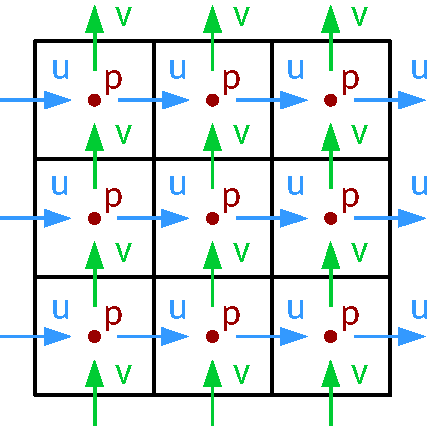
\includegraphics[width=0.3\textwidth]{StaggeredGrid.pdf}
	\caption[Staggered Grid]{Staggered grid: placement of the pressure and of the velocity components.}
	\label{StaggeredGrid}
\end{figure}\noindent
To avoid chequerboard instabilities, a staggered grid is used: the pressure is located at the centre of a cell, while the components of the velocity are placed at the cell faces, as shown in figure \ref{StaggeredGrid}. This technique was first proposed in \cite{harlow1965numerical}. The centred finite difference gradient operator applied to a cell-centred variable places the resulting vector field at the cell faces. The discrete divergence operator applied to a vector field whose components are at the cell faces, produces a cell-centred scalar field. The two operators are represented as sparse matrices in the code. The gradient matrix is obtained as the transpose of the divergence matrix, and the Laplacian matrix as their product.
% Linear system solution
\section{Linear System Solution}\label{Chapter_Solver_Section_Linear_System_Solution}
The weakly-compressible version of the code is integrated in time explicitly. This is not possible in the incompressible version. While steps \eqref{ChorinClassic_01} and \eqref{ChorinClassic_03} of the projection scheme can be explicit, the Poisson equation for the pressure \eqref{ChorinClassic_02} requires the solution of a linear system of equations.\par
For this purpose, the open source library PETSc \cite{petsc-user-ref}\cite{petsc-web-page}, (Portable, Extensible Toolkit for Scientific Computation) developed by Argonne National Laboratory, was integrated into the code. This library, written in C, is optimized for parallel scalability, hence responding to the needs of Grid-flow. PETSc offers many options for solving linear systems. For Grid-flow, the restarted GMRES (Generalized Minimal Residual) method coupled with an algebraic multigrid  was chosen.\par
It was shown by Vittoz \cite{Vittoz2018} that, while the need to solve the pressure Poisson equation in the incompressible formulation increases the CPU time needed for an individual time-step, compared to the weakly-compressible formulation, it does not impact excessively the parallel scalability of the code.
% Time integration 
\section{Time Integration}\label{Chapter_Solver_Section_Time_Integration}
At present, two time integration options exist in Grid-flow: forward Euler and a fourth-order Runge-Kutta scheme. The latter is characterized by the Butcher table: %(tableau?)
\begin{equation}
\begin{array}{c|cccc}
0 &  &  &  & \\
1 / 2 & 1 / 2 &  &  & \\
1 / 2 & 0 & 1 / 2 &  & \\
1 & 0 & 0 & 1 & \\
\hline
 & 1 / 6 & 1 / 3 & 1 / 3 & 1 / 6
\end{array}\label{RK4_Butcher}
\end{equation}
In the incompressible version, all steps of the projection scheme are executed for each stage of the Runge-Kutta algorithm.
% Finite volumes formulation
\section{Finite Volumes Formulation}\label{Chapter_Solver_Section_Finite_Volumes_Formulation}
\begin{comment}
A set of hyperbolic equations can be re-formulated as:
\begin{equation}
\dfrac{\partial\boldsymbol{W}}{\partial t}+\nabla\cdot\boldsymbol{\Psi}\left(\boldsymbol{W}\right)=\boldsymbol{S}\,,\label{HyperbolicSystem_commented}
\end{equation}
where the vector $\boldsymbol{W}$ collects all the conserved quantities, tensor $\boldsymbol{\Psi}\left(\boldsymbol{W}\right)$ represents the fluxes, and $\boldsymbol{S}$ is a source term. The systems of equations \eqref{ComprNS} and \eqref{IncomprNS}, while not strictly hyperbolic in nature, can still be re-formulated in the same way by defining the viscous fluxes $\boldsymbol{\Psi}_{v}\left(\boldsymbol{W}\right)=\boldsymbol{\tau}$ in addition to the advective ones.\par
\end{comment}
The systems of equations \eqref{ComprNS} and \eqref{IncomprNS} can be re-formulated as:
\begin{equation}
\dfrac{\partial\boldsymbol{W}}{\partial t}+\nabla\cdot\boldsymbol{\Psi}\left(\boldsymbol{W}\right)=\boldsymbol{S}\,,\label{HyperbolicSystem}
\end{equation}
where the vector $\boldsymbol{W}$ collects all the conserved quantities, tensor $\boldsymbol{\Psi}\left(\boldsymbol{W}\right)=\boldsymbol{\Psi}_{c}\left(\boldsymbol{W}\right)+\boldsymbol{\Psi}_{v}\left(\boldsymbol{W}\right)$ represents the fluxes, and $\boldsymbol{S}$ is the source term.  For the incompressible formulation, $\boldsymbol{W}= \boldsymbol{u}$, $\boldsymbol{\Psi}_{c}\left(\boldsymbol{W}\right)=-\boldsymbol{u}\otimes\boldsymbol{u}$ and $\boldsymbol{\Psi}_{v}\left(\boldsymbol{W}\right)=\boldsymbol{\tau}$. In the context of the projection scheme, the pressure gradient is part of the source term.\par
The \textit{finite volume} method for solving a set of PDEs considers a partitioning of the computational domain into a set of geometrical elements, or control volumes:
\begin{equation}
\Omega=\bigcup_{i=1}^{N}\Omega_{i}\,.
\end{equation}
Integrating \eqref{HyperbolicSystem} over a control volume $\Omega_{i}$, then applying Reynolds' transport theorem to the time derivative and the divergence theorem to the fluxes tensor produces:
\begin{equation}
\dfrac{\mathrm{d}}{\mathrm{d}t}\int_{\Omega_{i}}\boldsymbol{W}\mathrm{d}\Omega-\int_{\partial\Omega_{i}}\boldsymbol{W}\left(\boldsymbol{u}_{\Omega_{i}}\cdot\boldsymbol{n}\right)\mathrm{d}S+\int_{\partial\Omega_{i}}\boldsymbol{\Psi}\left(\boldsymbol{W}\right)\cdot\boldsymbol{n}\mathrm{d}S=\int_{\partial\Omega_{i}}\boldsymbol{S}\mathrm{d}\Omega\,,
\end{equation}
where $\boldsymbol{u}_{\Omega_{i}}$ is the speed of the frontier of the control volume. For fixed control volumes, this value is null.\par
The frontier of each control volume can be expressed as: $\partial\Omega_{i}=\bigcup_{j=1}^{M}A_{ij}$, therefore:
\begin{equation*}
\int_{\partial\Omega_{i}}\boldsymbol{\Psi}\left(\boldsymbol{W}\right)\cdot\boldsymbol{n}\mathrm{d}S=\sum_{j=1}^{M}\int_{A_{ij}}\boldsymbol{\Psi}\left(\boldsymbol{W}\right)\cdot\boldsymbol{n}\mathrm{d}S=\sum_{j=1}^{M}\boldsymbol{F}_{ij}\,A_{ij}\,,
\end{equation*}
where $\boldsymbol{F}_{ij}$ is the \textit{numerical flux} across face $A_{ij}$. Defining the volume averages:
\begin{equation*}
\boldsymbol{\overline{W}}_{i}=\dfrac{1}{\Omega_i}\int_{\Omega_{i}}\boldsymbol{W}\mathrm{d}\Omega\,;\qquad\qquad\qquad\boldsymbol{\overline{S}}_{i}=\dfrac{1}{\Omega_i}\int_{\Omega_{i}}\boldsymbol{S}\mathrm{d}\Omega\,;
\end{equation*}
\eqref{HyperbolicSystem} 
ten as:
\begin{equation}
\dfrac{\mathrm{d}\boldsymbol{\overline{W}}_{i}}{\mathrm{d}t}=-\sum_{j=1}^{M}\dfrac{A_{ij}}{\Omega_{i}}\boldsymbol{F}_{ij}+\boldsymbol{\overline{S}}_{i}\,,\label{HyperbolicCVDiscrete}
\end{equation}
therefore transforming a continuous PDE into a set of discrete relations between the volume-averaged values $\overline{\boldsymbol{W}}_{i}$.\par
Two aspects remain to be defined: how the domain is partitioned into control volumes, and how the numerical fluxes $\boldsymbol{F}_{ij}$ are reconstructed from the volume-averaged values $\overline{\boldsymbol{W}}_{i}$.
% Grid Management
\section{Grid Management}\label{Chapter_Solver_Section_Grid_Management}
The finite volume formalism can be applied to control volumes of any shape. In fact, it is commonly used by commercial CFD software based on unstructured grids.\par
Grid-flow, on the other hand uses rectangular control volumes (in two dimensions) or rectangular prisms (in three dimensions).
\begin{figure}[!ht]
	\centering
	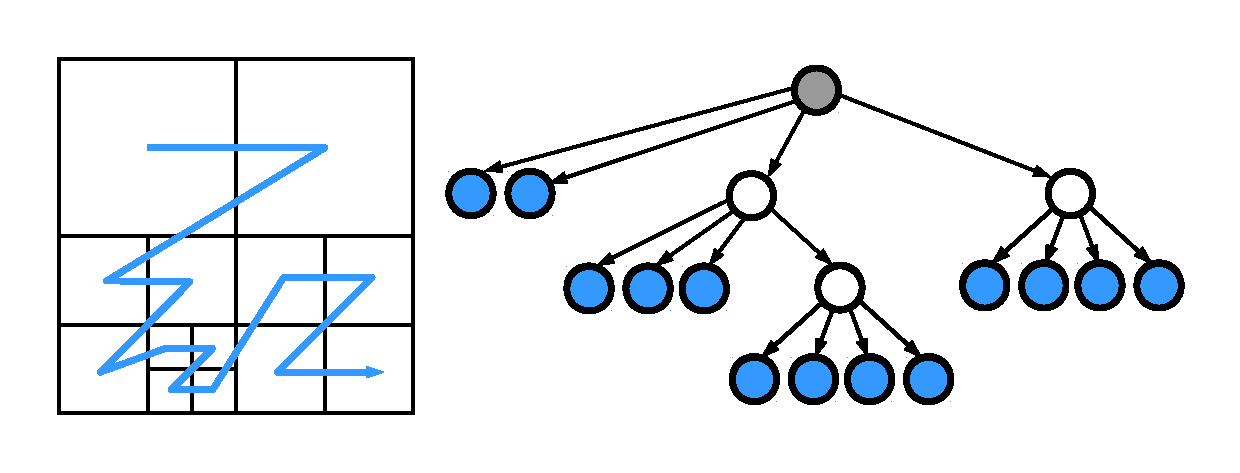
\includegraphics[height=0.4\textwidth]{MultilevelGridAndQuadtree.pdf}
	\caption[Multilevel Grid and Quadtree]{An example of two-dimensional multi-level Cartesian grid, showing the Z-order curve and the quadtree structure.}
	\label{MultilevelGridAndQuadtree}
\end{figure}\noindent
The computational domain is partitioned recursively into blocks, with the first block corresponding to the whole domain. In subsequent refinement passages, each block is subdivided into four (or eight, in three dimensions) smaller \textit{children} blocks until the desired level of refinement is reached. Blocks generated in this way are naturally organized in a quadtree (or octree, in three dimensions) graph, originating from the initial (root) block. Blocks that have no children are marked as leaf blocks. These blocks are not necessarily at the same level of refinement, as refinement criteria can vary across the domain, however, neighbouring blocks cannot differ in their level of refinement of more than one.\par
The leaf blocks are ordered in memory so that they follow a Z-order curve in the domain. This allows for an efficient way to refer to their position: interleaving the binary representations of their spatial coordinates returns their position (Morton key) along the Z-order curve.\par
\begin{figure}[!ht]
	\centering
	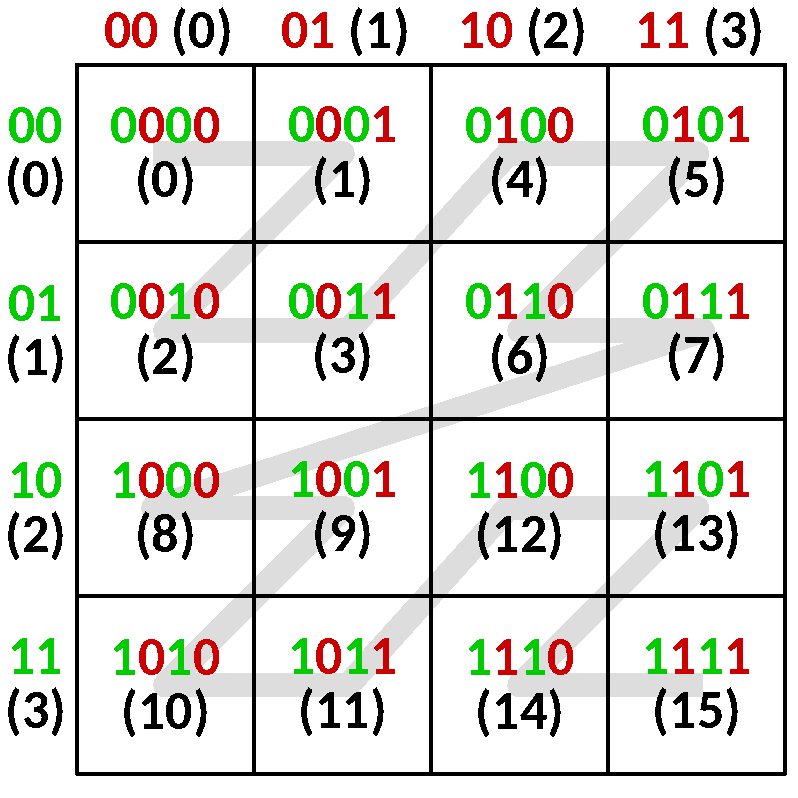
\includegraphics[width=0.3\textwidth]{MortonKeys.pdf}
	\caption[Morton Keys]{How the interleaving of binary coordinates produce the Morton keys.}
	\label{MortonKeys}
\end{figure}\noindent
Leaf blocks are further divided into a fixed number of cells, with a minimum of two per direction. These cells constitute the control volumes over which the finite volume formalism is applied.\par
This method of adaptive mesh refinement (or AMR) is very versatile in semi-automatically producing a grid which is refined locally where needed, while still preserving the convenience of the Cartesian structure.
% Parallelization
\section{Parallelization}
The Z-order curve preserves locality. This means that, partitioning the domain along it, subdomains constituted by (mostly) adjacent blocks are obtained, which is of great aid for parallelization.\par
The MPI library uses a \textit{distributed memory} model: the execution of the program is split into semi-independent processes, each acting on a portion of the data and exchanging information at specific points in the algorithm. Parallel performance is negatively affected by the amount of information exchanged between processes, which should be kept to a minimum. This is due to data transfer between processors being slower than data transfer between a processor and its allotted memory.\par
Another aspect of parallelization is whether communication between processes is synchronous or asynchronous. In synchronous communication the execution of a process stops at every communication event, until its completion. Grid-flow employs asynchronous communication: execution continues normally after data is sent to a different process, stopping only if required data has not been received yet.\par
Each process is allotted an equal number of blocks. The blocks in a process can be classified as local, inner and outer ones. Local and inner blocks are the ones in which each process performs operations, with inner blocks being at the boundaries of the subdomain allotted to the process. Outer blocks correspond to the inner blocks of the adjacent processes, and contain information needed to operate on the inner blocks. In short, each process sends the data of its inner blocks to the others, and fills its outer blocks with the data received from them.
\begin{figure}[!ht]
	\centering
	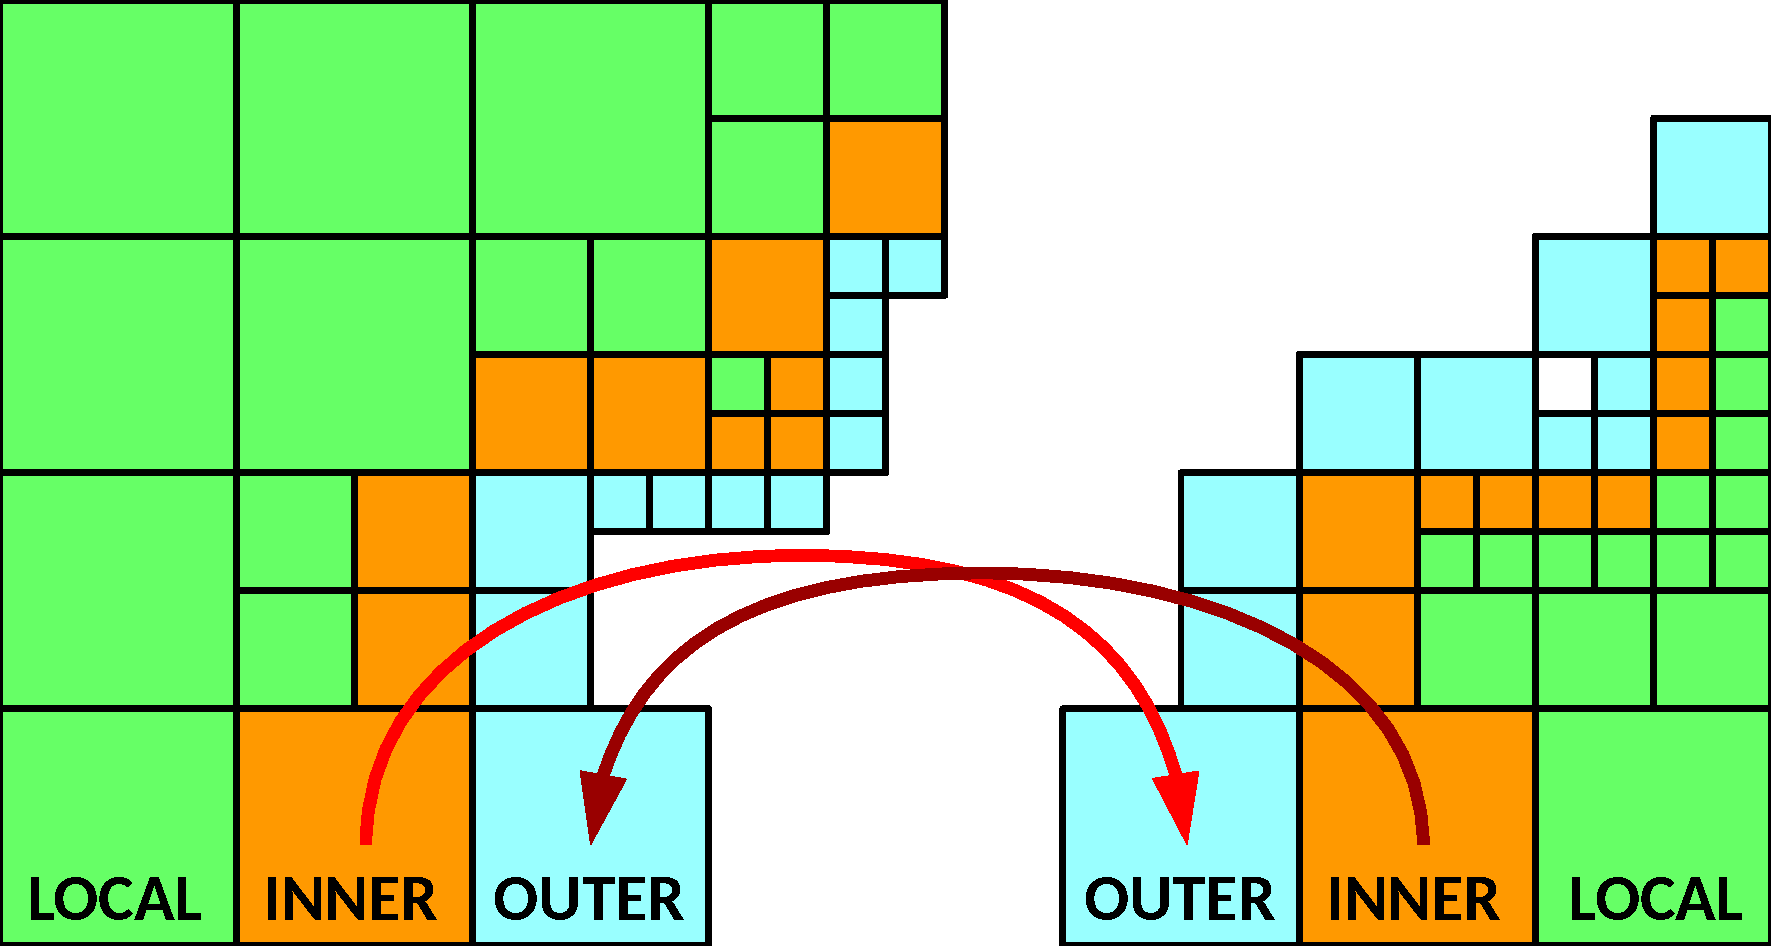
\includegraphics[width=0.55\textwidth]{LocalInnerOuter.pdf}
	\caption[Local, Inner and Outer Blocks]{The subdivision into local, inner and outer blocks in a process: inner and outer values are exchanged between processes.}
	\label{LocalInnerOuter}
\end{figure}\noindent
Each communication event in Grid-flow follows roughly the same steps:
\begin{enumerate}
	\item Any operation is performed first on the inner blocks. Grid-flow's explicit nature means that all required data is already present.
	\item Updated information from the inner blocks is sent to the other processes.
	\item The operation is performed on the local blocks. This part does not require any inter-process communication.
	\item Updated information for the outer blocks is received by the other processes. 
\end{enumerate}
Asynchronous execution means that different processes can be at different stages of an operation. Inner blocks are operated on, and their data sent as soon as possible so that, if any process is ahead of the sending one, it can receive the data it needs and continue. Operations on the local blocks (which take most of the computational time) are performed before the receiving step to give time to any process that may be lagging behind to send its inner block data.\par
It should be noted that if processes run at significantly different speeds, the code will only run as fast as the slowest one. However, for the unavoidable variations in speed that are to be expected during a computation, this strategy reduces idle times.\par
One operation that does not employ the scheme above is the solution of the pressure equation. The PETSc library is designed to operate as a "black box", although it employs distributed memory and asynchronous communications as well.\par
With PETSc, parallel vectors are defined, whose elements are distributed among all processes. It is possible to define the overall size of the vector and let PETSc decide how to spread it, or to define the size of its portions for each process. The second option is employed in Grid-flow, which allows each process to interact with the portion of a PETSc vector corresponding to its subdomain. 
Central to PETSc is also the definition of parallel sparse matrices, whose rows are spread among processes. These are stored in memory efficiently by keeping track of non-zero values only, and of their positions in the matrices. However, if the non-zero pattern of a sparse matrix changes, it will have to be reallocated in memory, at a performance cost. 
% Numerical fluxes
\section{Numerical Fluxes}\label{Chapter_Solver_Section_Numerical_Fluxes}
Control volumes in Grid-flow, as mentioned in \ref{Chapter_Solver_Section_Grid_Management}, are either rectangles or rectangular prisms. This means that equation \eqref{HyperbolicCVDiscrete} can be re-written as:
\begin{IEEEeqnarray}{cccccc}
\dfrac{\mathrm{d}\boldsymbol{\overline{W}}_{i,j,k}}{\mathrm{d}t}&=&-&\dfrac{\cancel{\Delta y\Delta z}}{\Delta x\cancel{\Delta y\Delta z}}\left(\boldsymbol{F}_{i+\frac{1}{2},j,k}-\boldsymbol{F}_{i-
	\frac{1}{2},j,k}\right)&-&\nonumber\\
&&-&\dfrac{\cancel{\Delta z\Delta x}}{\Delta y\cancel{\Delta z\Delta x}}\left(\boldsymbol{G}_{i,j+\frac{1}{2},k}-\boldsymbol{G}_{i,j-
	\frac{1}{2},k}\right)&-&\label{HyperbolicFVCartesian}\\
&&-&\dfrac{\cancel{\Delta x\Delta y}}{\Delta z\cancel{\Delta x\Delta y}}\left(\boldsymbol{H}_{i,j,k+\frac{1}{2}}-\boldsymbol{H}_{i,j,k-
	\frac{1}{2}}\right)&+&\boldsymbol{\overline{S}}_{i,j,k-
	\frac{1}{2}}\,,\nonumber
\end{IEEEeqnarray}
where $\boldsymbol{F}$, $\boldsymbol{G}$ and $\boldsymbol{H}$ are the fluxes along the cartesian directions, as shown in figure \ref{CellFluxes}. 
\begin{figure}[!ht]
	\centering
	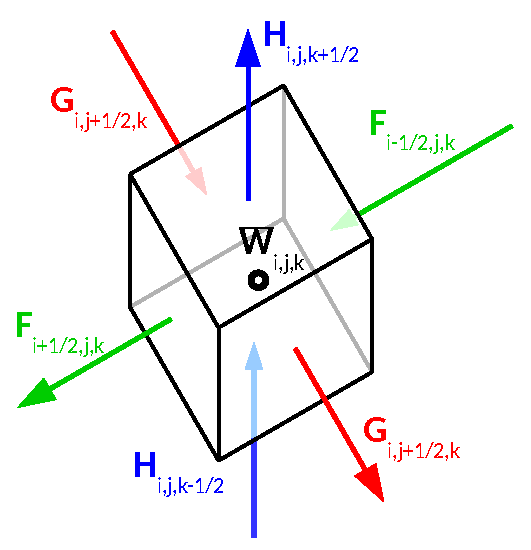
\includegraphics[width=0.35\textwidth]{CellFluxes.pdf}
	\caption[Numerical Fluxes]{The numerical fluxes entering and exiting of a three dimensional control volume.}
	\label{CellFluxes}
\end{figure}\noindent
If one were to substitute the fluxes with the values of $\boldsymbol{\Psi}\left(\boldsymbol{\overline{W}}_{i,j,k}\right)$ at the adjacent cells, the terms on the right-hand-side of equation \eqref{HyperbolicFVCartesian} would reduce to centred finite differences. This is problematic as it causes instability. Considering the one-dimensional transport equation:
\begin{equation}
\dfrac{\partial y}{\partial t}+u\dfrac{\partial y}{\partial x}=0\,,\label{1DTransport}
\end{equation}
it is easy to show that a centred forward Euler scheme in the form:
\begin{equation}
y^{n+1}_{i}-y^{n}_{i}=-u\dfrac{\Delta t}{2\Delta x}\left(y^{n}_{i+1}-y^{n}_{i-1}\right)\label{OrroreInstabile}
\end{equation}
is unconditionally unstable. This brings the necessity of breaking the symmetry in the stencil for the right-hand side. The usual strategy is \textit{upwinding}: given that the velocity field identifies a propagation direction for information, the sign of the velocity can be used to chose which direction to skew the stencil. For \eqref{1DTransport}, this can be done as:
\begin{subequations}\label{Upwinding}
\begin{IEEEeqnarray}{ccccc}
	y^{n+1}_{i}-y^{n}_{i}&=&-u\dfrac{\Delta t}{\Delta x}\left(y^{n}_{i+1}-y^{n}_{i}\right)&\qquad\mathrm{if}\,&u<0\,,\\
	y^{n+1}_{i}-y^{n}_{i}&=&-u\dfrac{\Delta t}{\Delta x}\left(y^{n}_{i}-y^{n}_{i-1}\right)&\qquad\mathrm{if}\,&u>0\,,
\end{IEEEeqnarray}
\end{subequations}
which is first order accurate in space, as opposed to the second order accuracy of a centred difference, but stable for sufficiently low $\Delta t / \Delta x$ ratios.\par
One aspect of upwinding is the introduction of numerical diffusion, which contributes to stability by damping spurious oscillations. However, excessive damping may penalize the accuracy of the solution.\par
In Grid-flow, at each interface between cells two fluxes are reconstructed: a left value, computed on a stencil centred on the cell on the left of the interface, and a right value, computed on a stencil centred on the cell on the right (figure \ref{LeftRightFluxes}).\par
\begin{figure}[!ht]
	\centering
	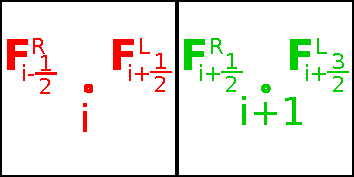
\includegraphics[width=0.25\textwidth]{LeftRightFluxes.pdf}
	\caption[Left and Right Fluxes]{Left and right reconstructed fluxes at the interface between two cells.}
	\label{LeftRightFluxes}
\end{figure}\noindent
The flux that goes into \eqref{HyperbolicFVCartesian} is, in general, a combination of the left and right values, that keeps into account the local signs of $\boldsymbol{W}$. Many options are implemented in Grid-flow for this combination, referred to as \textit{hyperbolic solvers}, however, for the incompressible formulation, the flux is simply chosen as:
\begin{subequations}
\begin{IEEEeqnarray}{rcclcc}
	&\boldsymbol{F}_{i+\frac{1}{2},j,k}&\,=\,&\boldsymbol{F}_{i+\frac{1}{2},j,k}^{L}&\qquad\mathrm{if}\,&u_{i+\frac{1}{2},j,k}>0\,,\\
	\smash{\left\{\IEEEstrut[12\jot]\right.}&\boldsymbol{F}_{i+\frac{1}{2},j,k}&\,=\,&\dfrac{1}{2}\left(\boldsymbol{F}_{i+\frac{1}{2},j,k}^{L}+\boldsymbol{F}_{i+\frac{1}{2},j,k}^{R}\right)&\qquad\mathrm{if}\,&u_{i+\frac{1}{2},j,k}=0\,,\\
	&\boldsymbol{F}_{i+\frac{1}{2},j,k}&\,=\,&\boldsymbol{F}_{i+\frac{1}{2},j,k}^{R}&\qquad\mathrm{if}\,&u_{i+\frac{1}{2},j,k}<0\,,
\end{IEEEeqnarray}
\end{subequations}
with analogous expressions for the other two directions. It should be noted that, for the advective fluxes in equation \eqref{IncomprNS_Momentum}, the sign check on the velocity should be performed at the faces of the staggered control volumes. For the fluxes in the normal direction, the average of the left and right reconstructed values of the normal velocity is used. For the tangential directions, the values of the tangential velocity require a further averaging step due to the staggered grid.\par
What is still left undefined is how the left and right reconstructions are computed. 
The various flux reconstruction schemes implemented in Grid-flow are presented in the remainder of this section.
\subsection{First Order Scheme}\label{First_Order_Scheme} 
The simplest possible strategy is using the values at the centre of the left cell for the left flux and the one in the right cell for the right flux. This would produce a first order accurate approximation analogous to \eqref{Upwinding}.\par 
\subsection{MUSCL}
MUSCL stands for Monotonic Upstream-centred Scheme for Conservation Laws. Its implementation in Grid-flow is described in \cite{Bigay2015}. Given the variable $u_{i}$, representing a generic quantity needing reconstruction at the cell faces, the MUSCL scheme defines the left and right fluxes as:
\begin{subequations}\label{MUSCL_Fluxes}
	\begin{IEEEeqnarray}{rccrcl}
		&u_{i-\frac{1}{2}}^{R}&\,=\,&u_{i}&\,-\,&\dfrac{1}{2}\Theta\left(\kappa_{i}\right)\left(u_{i+1}-u_{i}\right)\,,\\
		[-0.3\normalbaselineskip]\smash{\left\{\IEEEstrut[9\jot]\right.}\nonumber\\[-0.3\normalbaselineskip]
		&u_{i+\frac{1}{2}}^{L}&\,=\,&u_{i}&\,+\,&\dfrac{1}{2}\Theta\left(\kappa_{i}\right)\left(u_{i+1}-u_{i}\right)\,,
	\end{IEEEeqnarray}
\end{subequations}
where $\kappa_{i}=\frac{u_{i}-u_{i-1}}{u_{i+1}-u_{i}}$ and the function $\Theta\left(\kappa\right)$ is referred to as \textit{limiter}. A vast array of limiters have been proposed over the years. A simple one implemented in Grid-flow is the \textit{Minmod} limiter: $\Theta\left(\kappa\right)=\mathrm{max}\left[0,\,\mathrm{min}\left(1,\,\kappa\right)\right]$. If the limiter satisfies certain conditions, the MUSCL scheme is second order accurate in space and total variation diminishing. 
\subsection{WENO}
WENO stands for Weighted essentially non-oscillatory. Originally proposed by Liu, Osher and Chan in 1994 \cite{Liu1994}, he idea at the base of the method is to consider three different stencils around a cell, as in figure \ref{WENOStencils}.\par
\begin{figure}[!ht]
	\centering
	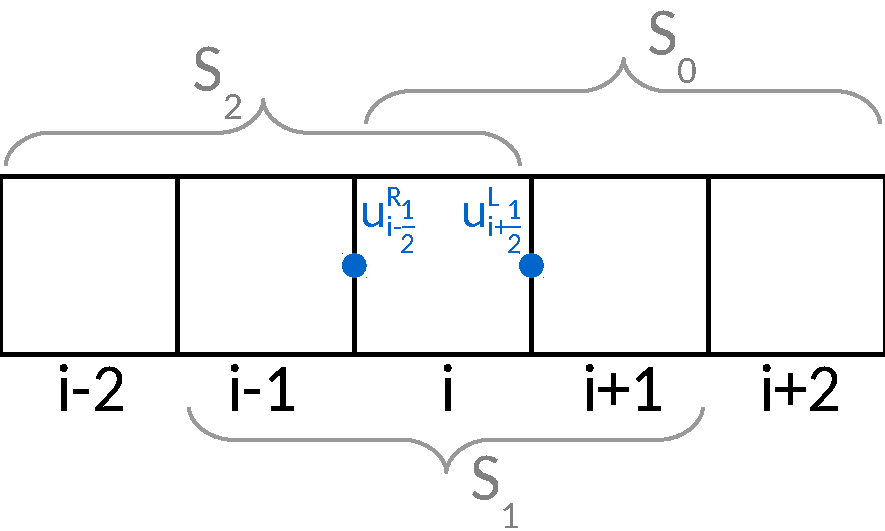
\includegraphics[width=0.5\textwidth]{WENO.pdf}
	\caption[Weno Stencils]{The three stencils used for the WENO reconstruction.}
	\label{WENOStencils}
\end{figure}\noindent
A third order accurate reconstruction of the values of $u$ at the cell faces is possible on each one of these stencils.\par
The reconstructed values are obtained as a weighted combination of these three approximations:
\begin{IEEEeqnarray}{rcccccl}\label{WENOFluxes}
	&u_{i+\frac{1}{2}}^{L}&\,=\,&\omega_{0}^{L}\left(\dfrac{1}{3}u_{i}+\dfrac{5}{6}u_{i+1}-\dfrac{1}{6}u_{i+2}\right)&\,+\,&\omega_{1}^{L}\left(-\dfrac{1}{6}u_{i-1}+\dfrac{5}{6}u_{i}+\dfrac{1}{3}u_{i+1}\right)&\,+\nonumber\\
	&&\,+\,&\omega_{2}^{L}\left(\dfrac{1}{3}u_{i-2}-\dfrac{7}{6}u_{i-1}+\dfrac{11}{6}u_{i}\right)&,&&\nonumber\\
	[-0.3\normalbaselineskip]\smash{\left\{\IEEEstrut[20\jot]\right.}&&&&&&\\[-0.3\normalbaselineskip]
	&u_{i-\frac{1}{2}}^{R}&\,=\,&\omega_{0}^{R}\left(\dfrac{11}{6}u_{i}-\dfrac{7}{6}u_{i+1}+\dfrac{1}{3}u_{i+2}\right)&\,+\,&\omega_{1}^{R}\left(\dfrac{1}{3}u_{i-1}+\dfrac{5}{6}u_{i}-\dfrac{1}{6}u_{i+1}\right)&\,+\nonumber\\
	&&\,+\,&\omega_{2}^{R}\left(-\dfrac{1}{6}u_{i-2}+\dfrac{5}{6}u_{i-1}+\dfrac{1}{3}u_{i}\right)&.&&\nonumber
\end{IEEEeqnarray}
The base values of the weights are: $d_{0}^{L}=\frac{3}{10}$, $d_{1}^{L}=\frac{3}{5}$, $d_{2}^{L}=\frac{1}{10}$, $d_{0}^{R}=\frac{1}{10}$, $d_{1}^{R}=\frac{3}{5}$, and $d_{2}^{R}=\frac{3}{10}$.\par
With $\omega_{i}^{L}=d_{i}^{L}$ and $\omega_{i}^{R}=d_{i}^{R}$ for $i=0,\,1,\,2$, reconstructions \eqref{WENOFluxes} would make \eqref{HyperbolicFVCartesian} fifth order accurate. The weights, however, are chosen in order to penalize or prioritize certain stencils, based on how regular $u$ is on them. The three regularity indicators
\begin{IEEEeqnarray}{rccccl}\label{WENORegularityIndexes}
	&\mathrm{IS}_{0}&\,=\,&\dfrac{13}{12}\left(u_{i+2}-2u_{i+1}+u_{i}\right)^{2}&\,+\,&\dfrac{1}{4}\left(u_{i+2}-4u_{i+1}+3u_{i}\right)^{2}\,,\nonumber\\
	\smash{\left\{\IEEEstrut[14.\jot]\right.}&\mathrm{IS}_{1}&\,=\,&\dfrac{13}{12}\left(u_{i+1}-2u_{i}+u_{i-1}\right)^{2}&\,+\,&\dfrac{1}{4}\left(u_{i+1}-u_{i-1}\right)^{2}\,,\\
	&\mathrm{IS}_{2}&\,=\,&\dfrac{13}{12}\left(u_{i}-2u_{i-1}+u_{i-2}\right)^{2}&\,+\,&\dfrac{1}{4}\left(3u_{i}-4u_{i-1}+u_{i-2}\right)^{2}\nonumber
\end{IEEEeqnarray} 
are defined, and the weights are computed as:
\begin{equation}
	\alpha_{i}=\dfrac{d_{i}^{L}}{\mathrm{IS}_{i}+\varepsilon}\,,\qquad\qquad \omega_{i}^{L}=\dfrac{\alpha_{i}}{\sum_{j=1}^{3}\alpha_{j}}\,,\qquad\qquad i=0,\,1,\,2\,,\label{WENOWeights}
\end{equation}
whth $\varepsilon=10^{-6}$ to avoid divisions by zero, and the same procedure applied to $\omega_{i}^{R}$.\par
This weight definition is meant to prevent oscillations due to discontinuities in the solution. A discontinuity in $u$ would cause the local regularity indicator to spike in value, in turn reducing the weight associated to the corresponding stencil. \eqref{WENOFluxes} would still produce a third order accurate approximation while avoiding the discontinuity altogether. On more regular portions of $u$, the indicators would be lower and the weights closer to their default values, allowing the reconstruction \eqref{WENOFluxes} to reach (ideally) fifth-order accuracy.\par
In Grid-flow, the implementation allows the user to chose whether to use the smoothness indicators or not. If they are active, the reconstruction is performed as described above. If not, the weights are automatically set to their default values for fifth order accuracy.\\\\
The previous discussion presupposes a uniform grid, however, this is not always the case in Grid-flow. Given that adjacent blocks differ by at most one level of refinement, and that they contain at least two cells per direction, the number of possible "configurations" is relatively limited.\par
For the weakly-compressible version of Grid-flow, coefficients for a variable-step WENO reconstruction are defined.\par
For the incompressible version of the code, things are further complicated by the adoption of the \textit{staggered} grid.\par
As shown in figure \ref{StaggeredGrid}, the components of the velocity are no longer placed at the centre of a cell but at its faces. On a uniform staggered grid, the control volumes for each component of the velocity are shifted along the corresponding direction, but maintain the same shape. While the fluxes along directions normal to the component of the velocity considered require some averaging, the WENO scheme is mostly unaltered. The situation is different for non-uniform grids, on which the staggering complicates the flux reconstruction procedure. The strategy adopted in Grid-flow consists in adapting the shape of the control volumes at the interfaces between different levels of refinement, and excluding some stencils.\par
The staggered grid causes an incompatibility between the WENO scheme used in the weakly-compressible formulation and the WENO scheme that had to be developed for the incompressible one.  
% Immersed Boundary
\section{Immersed Boundary}\label{Chapter_Solver_Section_Immersed_Boundary}
While not relevant at the present stage of this work, the immersed boundary technique implemented in the code deserves a mention.\par
At the base of the method is the definition, for each cell $i$, of a quantity $H_{i}$ representing the fraction of the cell volume occupied by the solid body. Ideally, its value is one inside the solid body, zero in the fluid and in between at the interface between them. 
The total momentum of a cell will be the sum of the momentum of the fluid and of that of the solid body, and the same will be true of its variation in time:
\begin{equation}
\left.\dfrac{\mathrm{d}\boldsymbol{u}_{i}}{\mathrm{d}t}\right|^{n}=\left(1-H_{i}\right)\left.\dfrac{\mathrm{d}\boldsymbol{u}_{i}}{\mathrm{d}t}\right|^{n}_{fluid}+H_{i}\left.\dfrac{\mathrm{d}\boldsymbol{u}_{i}}{\mathrm{d}t}\right|^{n}_{solid}\,,\label{IBM_01}
\end{equation}
where $\boldsymbol{u}_{i}\left(t\right)=\boldsymbol{u}\left(\boldsymbol{x}_{i},\,t\right)$, and assuming uniform density. The motion of the fluid is given by the time integration of the Navier-Stokes equations, while that of the solid is usually given:
\begin{equation*}
\left.\dfrac{\mathrm{d}\boldsymbol{u}_{i}}{\mathrm{d}t}\right|^{n}_{fluid}\approx\boldsymbol{RHS}^{n}_{i}\,,\qquad\qquad\qquad\left.\dfrac{\mathrm{d}\boldsymbol{u}_{i}}{\mathrm{d}t}\right|^{n}_{solid}\approx\boldsymbol{a}^{n}_{i}\,.
\end{equation*}
Combining the previous expressions gives:
\begin{equation}
\left.\dfrac{\mathrm{d}\boldsymbol{u}_{i}}{\mathrm{d}t}\right|^{n}\approx\left(1-H_{i}\right)\boldsymbol{RHS}^{n}_{i}+H_{i}\boldsymbol{a}^{n}_{i}=\boldsymbol{RHS}^{n}_{i}+\boldsymbol{S}^{n}_{i}\,,\label{IBM_02}
\end{equation}
with $\boldsymbol{S}^{n}_{i}=H_{i}\left(\boldsymbol{a}^{n}_{i}-\boldsymbol{RHS}^{n}_{i}\right)$ the force that the solid applies on the fluid. By substituting $\boldsymbol{RHS}^{n}_{i}$ and $\boldsymbol{a}^{n}_{i}$ with the finite difference expressions of the velocity time derivatives gives the alternative expression for $\boldsymbol{S}^{n}_{i}$:
\begin{equation}
\boldsymbol{S}^{n}_{i}=H_{i}\left(\dfrac{\left.\boldsymbol{u}_{i}^{n+1}\right|_{solid}-\boldsymbol{u}_{i}^{n}}{\Delta t}-\dfrac{\left.\boldsymbol{u}_{i}^{n+1}\right|_{fluid}-\boldsymbol{u}_{i}^{n}}{\Delta t}\right)=H_{i}\dfrac{\left.\boldsymbol{u}_{i}^{n+1}\right|_{solid}-\left.\boldsymbol{u}_{i}^{n+1}\right|_{fluid}}{\Delta t}\,,
\end{equation}
which shows that the force represents a "correction" of the velocity field.\par 
In practice, $H_{i}$ is smoothed around the interface. In Grid-flow, this is done using the regularized Heaviside function:
\begin{equation}
H\left(\phi\right)=\dfrac{1}{2}\left[1+\mathrm{tanh}\left(\alpha\dfrac{\phi}{\Delta x}\right)\right]\,,\label{DeltaFunctionIBM}
\end{equation}
where $\phi$ is the distance from the interface, $\Delta x$ the local cell size and $\alpha$ a parameter defining the span of the transition zone.\par
It should be noted that in the incompressible version of the code, two conflicting corrections are applied to the velocity field, one at the end of the projection scheme, to impose mass conservation, and one to account for the presence of the body. In \cite{Vittoz2018} the problem of which correction to apply first is considered.  
\begin{figure}[!ht]
	\centering
	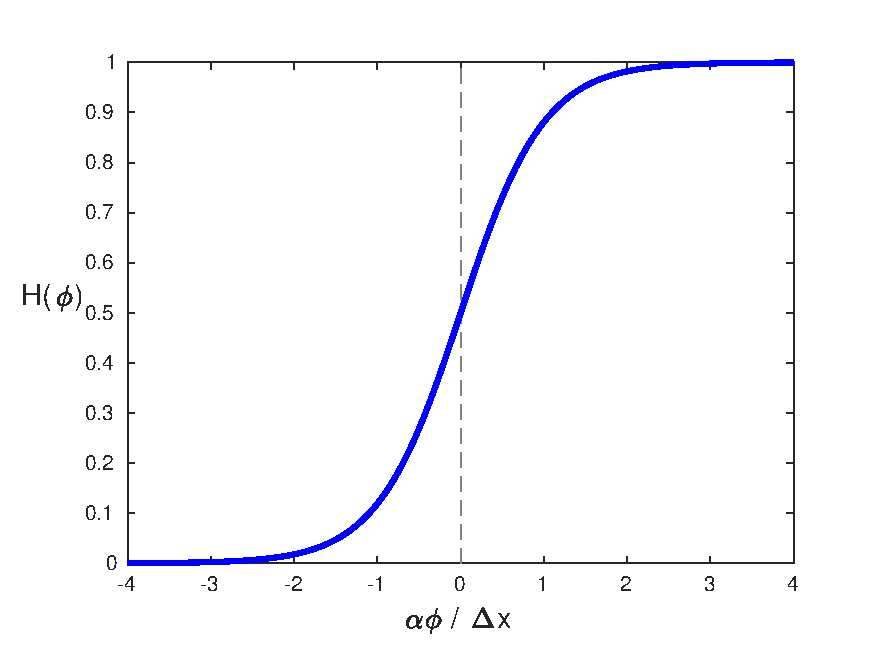
\includegraphics[width=0.65\textwidth]{Heaviside.eps}
	\caption[Regularized Heaviside function]{The regularized Heaviside function \eqref{DeltaFunctionIBM}.}
	\label{Heaviside}
\end{figure}\noindent
%----------------------------------------------- CHAPTER 3 ------------------------------------------------------------------------------------
\chapter{Multiphase flows}\label{Chapter_Multiphase_Flows}
In this context, a multiphase flow is defined as a flow involving two (or more) immiscible fluids, having different properties (i.e. density, viscosity).\par
Hirt and Nichols, in their original article presenting the Volume of Fluid method \cite{hirt1981volume}, proposed a breakdown of the problem of simulating multiphase flows into three main aspects:
\begin{itemize}
\item Numerical description of the location and shape of the boundary between the fluids.
\item Evolution algorithm for the boundary.
\item Scheme for imposing boundary conditions at the interface.
\end{itemize}
% ~~~~~~~~~~~~~~~~~~~~~~ History
\section{Numerical description of the boundary}
Numerous strategies exist for describing the evolution of the interface between the fluids, with many variations and hybrid approaches between them. A first distinction can be made between Lagrangian methods, in which the interface is followed directly, and Eulerian methods, in which an additional quantity is introduced to keep track of the interface. The two principal Eulerian methods are the Volume-of-Fluid method and the Level Set method.
% Lagrangian methods
\subsection{Lagrangian Methods}
For codes that employ an Eulerian description of the flow, massless particles can be added and advected in order to follow the interface's movement. One of the earliest examples is the Marker and Cell method developed by Harlow and Welch \cite{harlow1965numerical}. While initially developed to tackle free-surface problems, this method is easy to adapt to multiphase flows: one of the fluids is initially filled with a large number of massless particles, which are then advected, keeping track of where the tagged fluid is. This method is expensive, as it requires a great number of advected particles in order to be precise.\par
\begin{comment}
\begin{figure}[!ht]
	\centering
	
\includegraphics[width=0.35\textwidth]{placeholder.pdf}
	\caption[volume tracking vs. Surface tracking]{On the left, volume tracking particles; on the right, surface tracking particles.}
	\label{VolumeSurfaceTracking}
\end{figure}\noindent
\end{comment}
An alternative is the use of massless particles to tag the interface itself (surface tracking), rather than one of the fluids (volume tracking). This reduces the number of particles needed. However, in this case the interface is known through a set of discrete points, with no information on their connectivity. This is particularly problematic for breaks in the interface.\par
In general, Lagrangian methods need to be coupled with techniques to reconstruct the shape of the interface from the discrete set of particles, which can add considerable algorithmic complexity, especially in three dimensions.\par
Lagrangian methods can, on the other hand, be used in tandem with an Eulerian approach, with the two methods interacting through reciprocal corrections.\par
For mesh-free codes that employ a Lagrangian description of the fluid, such as the SPH (Smoothed-particle hydrodynamics) method, the particles on which the computation is based can be constituted of different fluids. The movement of the interface is then implicit in that of the fluid particles.
% Volume-of-Fluid
\subsection{Volume of Fluid Method}
The Volume-of-Fluid method, first proposed in \cite{hirt1981volume}, introduces a quantity $\alpha$ called \textit{volume fraction}. This quantity represents, for each cell in the discretized computational domain, how much of it is filled by one particular fluid.\par 
\begin{figure}[!ht]
	\centering
	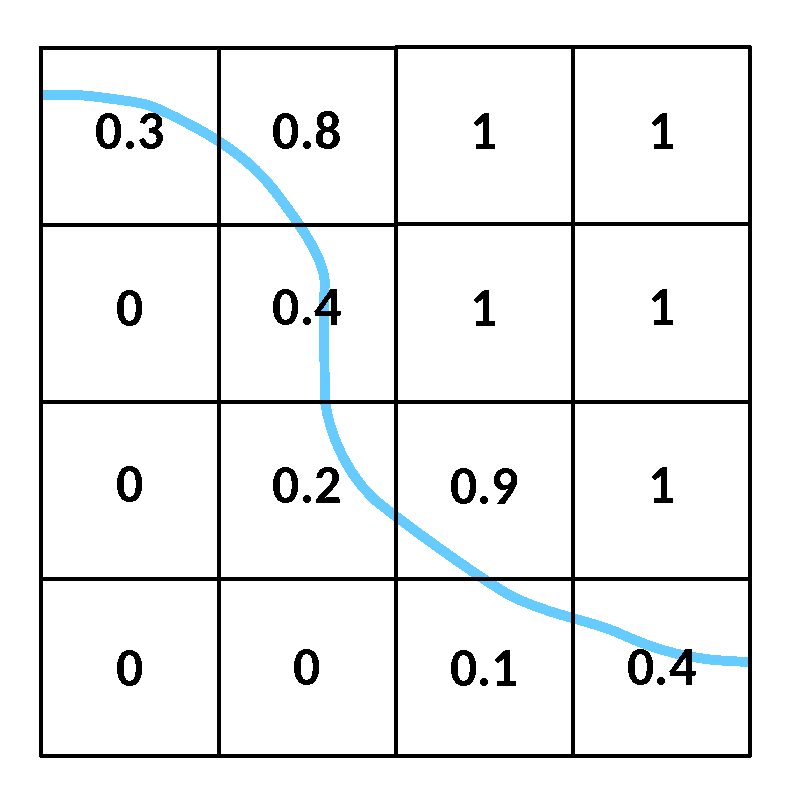
\includegraphics[width=0.35\textwidth]{VOF.pdf}
	\caption[Volume of Fluid]{Values of $\alpha$ around an interface.}
	\label{VOF}
\end{figure}\noindent
This method has the advantage that, as long as the quantity $\alpha$ is conserved, so is the mass of both fluids. The main disadvantage is that the actual position and shape of the interface is only known hazily.\par
In general keeping track of $\alpha$ is not sufficient, and a method for reconstructing the interface based on $\alpha$'s values is needed.\par
Numerous reconstruction methods have been proposed. An overview can be found in \cite{pilliod2004second} 
% Level-Set
\subsection{Level Set Method}
The Level Set method, first proposed by Osher and Sethian \cite{osher1988fronts} in 1988, defines a scalar field $\phi$, such that its zero level curve (or level surface, in three dimensions) represents the interface between the fluids:
\begin{equation}
\partial\Omega = \left\{\left.\boldsymbol{x}\right|\phi\left(\boldsymbol{x},\,t\right)=0\right\}\label{ZeroLevelCurve}
\end{equation}
Advecting the Level Set function as a passive scalar moves the zero level curve, and hence the interface, with the fluid. Unlike the volume fraction, the Level Set function does contain information on the position and shape of the interface. In fact, the normal $\boldsymbol{n}$ to the interface and its curvature $\kappa$ can be computed as:
\begin{equation}
\boldsymbol{n}=\dfrac{\nabla\phi}{\left|\nabla\phi\right|}\,,\qquad\qquad\qquad \kappa=-\nabla\cdot\left(\dfrac{\nabla\phi}{\left|\nabla\phi\right|}\right)\,.\label{LevelSetNormalCurvature}
\end{equation}
\begin{figure}[!ht]
	\centering
	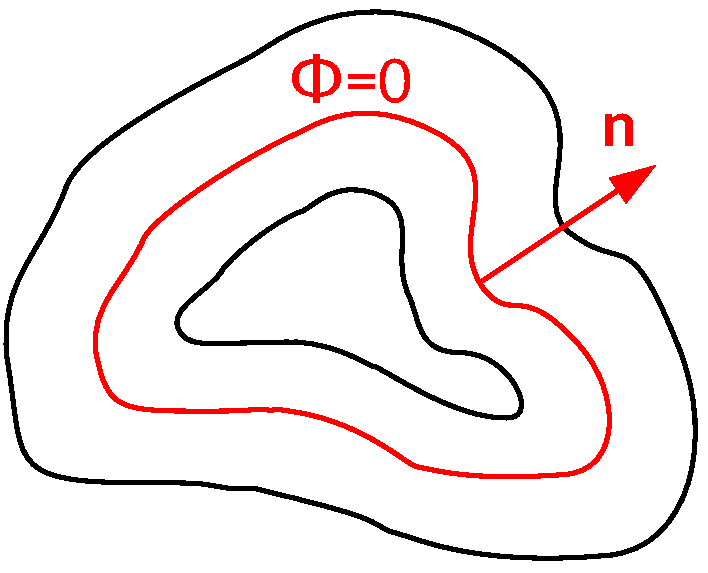
\includegraphics[width=0.35\textwidth]{LevelSet.pdf}
	\caption[level Set curve]{Level curves around an interface.}
	\label{LevelSet}
\end{figure}\noindent
Usually, but not exclusively, the Level Set function $\phi$ is defined as the \textit{signed distance} from the interface. This means that the value of $\phi$ conveys which fluid is present, while its value the distance from the border between the two fluids.\par
One characteristic of a distance field is that:
\begin{equation}
\left|\nabla\phi\right|=1\,.\label{LevelSetGradient}
\end{equation}
One downside of the Level Set is that, unlike the volume fraction, it is a geometrical quantity, not directly linked to the physical "amounts" of the two fluids, which can result in mass conservation problems.\par
It can be noted that the volume fraction $\alpha$ for a control volume $\Omega_{i}$ can be computed from the Level-Set function $\phi$:
\begin{equation}
	\alpha=\dfrac{1}{\Omega_{i}}\int_{\Omega_{i}}\mathrm{H}\left(\phi\right)\mathrm{d}\Omega\,,\qquad\mathrm{where}\qquad\mathrm{H}\left(\phi\right)=\left\{\begin{array}{rccl}
	1\,,&\;&\mathrm{if}\;&\phi>0\,,\\
	0\,,&\;&\mathrm{if}\;&\phi\leq 0\,.
	\end{array}\right.\label{CLSVOF}
\end{equation}
The inverse relation ($\alpha\rightarrow\phi$) is more complicated, but feasible to implement.\par
One possible strategy to overcome the mass conservation problems of the Level Set while preserving its advantages is to couple it with a volume of fluid method. The two methods can be used to correct each other through \eqref{CLSVOF} and its inverse. This strategy, named CLSVOF (for Conservative Level Set Volume of Fluid), is the one explored in the PhD work of Thibaut Menard \cite{Menard2007}. 
\section{Evolution algorithm for the boundary}
The movement of a fluid particle is described by the equation:
\begin{equation}
\left.\dfrac{\mathrm{d}\boldsymbol{x}}{\mathrm{d}t}\right|_{\boldsymbol{X},\,t}=\boldsymbol{u}\left(\boldsymbol{x}\left(\boldsymbol{X},\,t\right),\,t\right)\,.\label{AdvectionParticle}
\end{equation}
For Lagrangian methods, this expression can be integrated in time to keep track of massles particles. For Eulerian methods, quantities such as the volume fraction and the Level Set remain constant along the paths of individual particles, hence their material derivative is null:
\begin{equation}
\dfrac{\mathrm{D}\phi}{\mathrm{D}t}=\dfrac{\partial\phi}{\partial t}+\boldsymbol{u}\cdot\nabla\phi=0\,.\label{AdvectionEquation}
\end{equation}
However, for interface capturing methods, simply integrating \eqref{AdvectionEquation} in time may be problematic. Some amount of numerical diffusion is bound to be introduced by the finite arithmetic, causing smearing or distortion of the interface.\par
In volume-of-fluid methods, in general, specialized advection schemes are developed to ensure that $\alpha$ remains bounded between $0$ and $1$ and to avoid excessive diffusion.\par
In Level-Set methods, integration of \eqref{AdvectionEquation} will cause level curves to no longer be parallel, prompting $\phi$ to lose its meaning of signed distance. To restore it an additional passage is usually applied, in order to make the $\phi$ field satisfy \eqref{LevelSetGradient} again.\par
A common strategy is to consider the equation:
\begin{equation}
	\dfrac{\partial d}{\partial\tau}+\mathrm{sign}\left(\phi\right)\left(\left|\nabla d\right|-1\right)=0\,,\label{RedistantiationFunction}
\end{equation}
whose steady state is $\left|\nabla d\right|=1$. $d$ is initialized as equal to $\phi$, and $\phi$ is set equal to $d$'s final value. Few (pseudo-)time iterations are required for the level curves to become parallel again, at least close to the interface, where it is needed.\par
As discussed in \cite{hartmann2008differential}, the use of \eqref{RedistantiationFunction} comes with some caveats, such as the necessity for upwinding $\nabla d$.\par
The sign function is generally regularized as $\phi / \sqrt{\phi^{2}+\Delta x^{2}}$.
\section{Scheme for imposing boundary conditions at the interface}
Across the interface between two fluids there is a discontinuity in fluid properties, such as density and viscosity. Velocity is generally considered continuous across the interface, at least for viscous flows. Stresses acting on the fluid are not continuous across the interface due to surface tension:
\begin{equation}
	\left[\boldsymbol{\tau}\boldsymbol{n}-p\boldsymbol{n}\right]=-\sigma\kappa\boldsymbol{n}\,.
\end{equation}
In numerical schemes for incompressible flows, there are two main strategies to apply surface tension: as an impulsive  force in the momentum balance equation \eqref{IncomprNS_Momentum} or as a discontinuity in pressure. A detailed presentation of the jump conditions between two incompressible fluids can be found in \cite{kang2000boundary}.\par
The easiest way to handle discontinuities is to smear them through the use of regularized Heaviside functions, or \textit{delta functions}. Given the signed distance $\phi$ from the interface:
\begin{subequations}
\begin{IEEEeqnarray}{crcl}
	&\rho\left(\phi\right)&\,=\,&\rho_{1}+\left(\rho_{2}-\rho_{1}\right)H\left(\phi\right)\,,\label{DeltaFunctionDensity}\\
	\smash{\left\{\IEEEstrut[9\jot]\right.}&\mu\left(\phi\right)&\,=\,&\mu_{1}+\left(\mu_{2}-\mu_{1}\right)H\left(\phi\right)\,,\label{DeltaFunctionViscosity}\\
	&\boldsymbol{f}_{sf}\left(\phi\right)&\,=\,&\sigma\kappa\left(\phi\right)\nabla H\,.\label{DeltaFunctionSurfaceTension}
\end{IEEEeqnarray}
\end{subequations}
The function $H\left(\phi\right)$ can be, for example, \eqref{DeltaFunctionIBM}, however, a variant more commonly used in the multiphase flows literature \cite{BIHS2016191}\cite{kang2000boundary} is:
\begin{IEEEeqnarray}{rlrcl}
	&0&\quad\phi\,&<&\,-\varepsilon\,,\nonumber\\
	H\left(\phi\right)=\smash{\left\{\IEEEstrut[9\jot]\right.}&\dfrac{1}{2}+\dfrac{\phi}{2\varepsilon}+\dfrac{1}{2\pi}\mathrm{sin}\left(\dfrac{\pi\phi}{\varepsilon}\right)&\quad-\varepsilon\leq&\phi&\leq\varepsilon\,,\label{DeltaFunctionLS}\\
	&1&\quad\phi\,&>&\,\varepsilon\,.\nonumber
\end{IEEEeqnarray}
This method while simple, has the downside of creating an artificial interface thickness which impacts the accuracy of the solution.
An alternative to the use of delta functions is to modify the discrete operations to account for the jump conditions. One strategy that employs this strategy is the Ghost Fluid method, first proposed by Fedkiw et al. \cite{fedkiw1999non} in 1999. This method consists in extending each fluid across the interface of one (or more) cell(s). The values at these ghost cells are determined by imposing the satisfaction of the jump conditions. This method was adapted to the solution of the Poisson equation on a discontinuous domain in \cite{liu2000boundary}, and to a multiphasic incompressible fluid flow in \cite{kang2000boundary}. 

%----------------------------------------------- CHAPTER 4 ------------------------------------------------------------------------------------
\chapter{Implementation}\label{Chapter_Implementation}
In the current implementation of the weakly-compressible version of Grid-flow, a volume-of-fluid method for simulating multiphase flows exists. This scheme employs two different mass conservation equations for the two fluids, and derives the value of the volume fraction $\alpha$ by imposing that their partial pressures are at equilibrium \cite{Li2020}. Due to its reference to mass conservation equations involving density, and its use of an equation of state for finding the partial pressures, this method cannot be adapted to the incompressible formulation.\par
It was decided instead to implement a scheme based on the Level Set. The reasons are the method's relative simplicity and robustness, the vast literature dedicated to it and its many possible routes for improvement. Another reason is the opportunity to build on the previous implementation of the method by Am{\'{e}}lie Bardin \cite{Bardin2015} in an older version of Grid-flow.
The main interventions on the code were:
\begin{enumerate}
	\item Adaptation of the pre-existing Level-Set advection subroutines for the weakly-compressible version to the incompressible version. 
	\item Addition of the option to reinitialize the Laplacian matrix at every time step, and implementation of variable density inside the Poisson equation for the pressure.
	\item Coupling between the variable density and the Level-Set by implementing \eqref{DensityDeltaFunction} in the code.
\end{enumerate} 
% ~~~~~~~~~~~~~~~~~~~~~~~~~~~~ Method chosen
\section{Description of the Method}\label{Chapter_Implementation_Description_of_the_Method}
\subsection{The Level Set function}
In the context of a staggered grid, the Level Set function $\phi$ is placed at the center of the cell. Advection takes place integrating in time equation
\begin{equation}
\dfrac{\partial\phi}{\partial t}+\nabla\cdot\left(\boldsymbol{u}\phi\right)=0\,,\label{LevelSetAdvectionConservative}
\end{equation}
which is the conservative form of \eqref{AdvectionEquation}. The two formulations are equivalent for incompressible flows, since $\nabla\cdot\boldsymbol{u}=0$, but \eqref{LevelSetAdvectionConservative} is more straightforward to implement in a finite volume formulation and is the one used in this work.\par
It should be noted that in the literature on the Level Set the non-conservative form \eqref{AdvectionEquation} is more commonly seen. In \cite{Zuzio2020}, \eqref{LevelSetAdvectionConservative} has the source term $\phi\nabla\cdot\boldsymbol{u}$ added on the right, in order to be compatible with \eqref{AdvectionEquation} if $\nabla\cdot\boldsymbol{u}=0$ is not satisfied exactly.\par
In Am{\'{e}}lie Bardin's work \cite{Bardin2015} both the conservative form \eqref{LevelSetAdvectionConservative} and the non-conservative form \eqref{AdvectionEquation} were tested, the latter in a finite difference formulation. The conservative form was kept as it performed better.\par
%For the present work the conservative form is used, with the finite volume formalism described in \ref{Chapter_Solver_Section_Finite_Volumes_Formulation}. 
Different flux reconstruction schemes were used for the Level Set during testing.\par
Time integration is performed with forward Euler or with the fourth order Runge-Kutta scheme presented in \ref{Chapter_Solver_Section_Time_Integration}.
\subsection{Discontinuity management}
In this work viscous effects are ignored, and no surface tension model was implemented, so the only discontinuity is in the density of the two fluids. The density jump is regularized through expression \eqref{DeltaFunctionDensity}, coupled with the Heaviside function \eqref{DeltaFunctionIBM}:
\begin{equation}
\rho\left(\phi\right)=\rho_{1}+\dfrac{\rho_{2}-\rho_{1}}{2}\left[1+\mathrm{tanh}\left(\alpha\dfrac{\phi}{\Delta x}\right)\right]\,.\label{DensityDeltaFunction}
\end{equation}
The non-uniform density affects the Poisson equation for pressure \eqref{ChorinClassic_02}:
\begin{equation}
	\nabla\cdot\left(\dfrac{1}{\rho}\nabla p\right)=\frac{1}{\Delta t}\nabla\cdot\boldsymbol{u}^{*}\,.\label{PoissonPressureVarDensity}
\end{equation}
It is easy to show in one dimension that, with centered finite differences, the values of the density are needed at the cell faces:
\begin{equation*}
	\left.\dfrac{\partial}{\partial x}\left(\dfrac{1}{\rho}\dfrac{\partial p}{\partial x}\right)\right|_{i}\approx\dfrac{1}{\Delta x}\left[\dfrac{1}{\rho_{i+\frac{1}{2}}}\dfrac{p_{i+1}-p_{i}}{\Delta x}-\dfrac{1}{\rho_{i-\frac{1}{2}}}\dfrac{p_{i}-p_{i-1}}{\Delta x}\right]\,,
\end{equation*}
however, the Level Set is stored at the cell centre. It is possible to apply \eqref{DensityDeltaFunction} to the Level-Set at the cell centres, then interpolate the density at the cell faces, or interpolate the Level Set first, and then compute the density. In \cite {BIHS2016191} both strategies are tested, with the former resulting in additional spurious (albeit stable) oscillations. In this work, the latter strategy is employed. In fact, the values of the Level Set are reconstructed at the cell faces when computing the fluxes for equation \eqref{LevelSetAdvectionConservative}. Their values are stored and then fed to \eqref{DensityDeltaFunction} to compute the density.
\subsection{Method summary}
Assuming integration in time is performed with forward Euler, and the non-incremental form of Chorin's projection method is used, the scheme can be summarized as:
\begin{subequations}
	\label{ChorinMulti}
	\begin{enumerate}
		\item Update the Level Set:
		\begin{equation}
			\dfrac{\phi^{n+1}-\phi^{n}}{\Delta t}=-\nabla\cdot\left(\boldsymbol{u}^{n}\phi^{n}\right)\,,\label{ChorinMulti_01}
		\end{equation}	
		\item Compute the intermediate velocity field: 
		\begin{equation}
		\dfrac{\boldsymbol{u}^{*}-\boldsymbol{u}^{n}}{\Delta t}=-\nabla\cdot\left(\boldsymbol{u}^{n}\otimes\boldsymbol{u}^{n}\right)+\boldsymbol{g}\,,\label{ChorinMulti_02}
		\end{equation}	
		\item Compute the density at the cell faces:
		\begin{equation}
			\rho\left(\phi^{n+1}\right)=\rho_{1}+\dfrac{\rho_{2}-\rho_{1}}{2}\left[1+\mathrm{tanh}\left(\alpha\dfrac{\phi^{n+1}}{\Delta x}\right)\right]\,,\label{ChorinMulti_03}
		\end{equation}
		\item Solve the variable coefficient Poisson equation for the pressure:
		\begin{equation}
			\nabla\cdot\left(\dfrac{1}{\rho\left(\phi^{n+1}\right)}\nabla p^{n+1}\right)=\frac{1}{\Delta t}\nabla\cdot\boldsymbol{u}^{*}\,,\label{ChorinMulti_04}
		\end{equation}
		\item Apply the pressure gradient to correct the vector field: 
		\begin{equation}
			\boldsymbol{u}^{n+1}=\boldsymbol{u}^{*}-\frac{\Delta t}{\rho\left(\phi^{n+1}\right)}\nabla p^{n+1}\,.\label{ChorinMulti_05}
		\end{equation}
	\end{enumerate}
\end{subequations}
The rationale behind using the density field at $t^{n+1}$ in \eqref{ChorinMulti_04} is given in \cite{kang2000boundary}: the solution of this equation is used to correct the updated velocity field $\boldsymbol{u}^{n+1}$.
\begin{comment}
\section{Level Set advection}\label{Chapter_Implementation_Section_Level_Set_advection}
Grid-flow is a code under active development, subject to frequent changes and updates. The developments presented here started in 2019 on a version of the code having some limitations to the flux reconstruction subroutines, that were lifted in a later (2020) release. For this reason, the advection scheme for the Level Set  in the incompressible formulation had to be implemented twice: initially in the 2019 version of the code, and later in the 2020 version, to take full advantage of its improvements.\par
As mentioned in section \ref{Chapter_Solver_Section_Numerical_Fluxes}, the use of a staggered grid in the incompressible formulation meant that the WENO scheme had to be substantially modified. In fact, the weakly-compressible and the incompressible versions of the code use different subroutines for the WENO reconstructions, with little inter-compatibility.\par
In the 2019 version of the code, the WENO scheme for cell-centred variables in use in the weakly-compressible formulation was not available to the incompressible formulation, where only face-centred variables needed flux reconstruction. The MUSCL scheme, at this point, was not compatible either with the incompressible formulation. The only option for the advection of cell-centred quantities in the incompressible version, already in use for the eddy viscosity of the Spalart-Allmaras turbulence model, was the first order scheme described in \ref{First_Order_Scheme}. This scheme was relatively easy to adapt to the advection of $\phi$. The first results were obtained on the 2019 version of the code, with this scheme used for advecting $\phi$. \par
In the more recent version of the code, the MUSCL scheme and WENO subroutines for cell-centred variables were made available to the incompressible formulation. This allowed their use for advecting the Level Set.\par
For pure transport tests the first order and the MUSCL schemes proved too dissipative, consistently with what was observed in \cite{Bardin2015}, while the WENO scheme preserved satisfactorily the shape of the interface.\par
For multiphasic tests, while still too dissipative, the first order and MUSCL schemes demonstrated an advantage over WENO in terms of stability.
\end{comment}
\section{Variable coefficient Poisson Equation}\label{Chapter_Implementation_Variable_Coefficient_Poisson_Equation}
\subsection{PETSc Projection Scheme}\label{Subsection_PETSc_projection_scheme}
\begin{figure}[!ht]
	\centering
	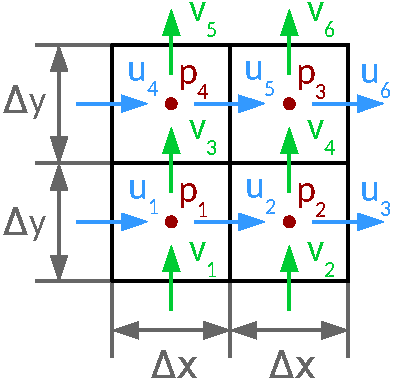
\includegraphics[width=0.3\textwidth]{StaggeredGrid4.pdf}
	\caption[Staggered Grid 4 cells]{A simple domain made of four staggered cells.}\label{StaggeredGrid4}
\end{figure}\noindent
In the single-fluid incompressible version of Grid-flow, all differential operators used to compute the pressure and its gradient are rebuilt every time there is a change in the grid. All sparse matrices are re-initialized, since their non-zero pattern depends on how the cells are distributed on the domain. 
The first operators to be built are the divergence matrices, one per direction.:
\begin{equation*}
\boldsymbol{D}_{x}\,;\qquad\boldsymbol{D}_{y}\,;\qquad\boldsymbol{D}_{z}\,.
\end{equation*}
They are built so that they perform centred finite differences on the face-centred variables, multiplied by the cell volume. For example, considering the four cells in figure \ref{StaggeredGrid4}, in 2D, $\boldsymbol{D}_{x}$ would take the form:
\begin{equation}
\boldsymbol{D}_{x}=\dfrac{\Delta y\cancel{\Delta x}}{\cancel{\Delta x}}\left[\begin{array}{cccccc}
-1 & 1 & 0 & 0 & 0 & 0\\
0 & -1 & 1 & 0 & 0 & 0\\
0 & 0 & 0 & -1 & 1 & 0\\
0 & 0 & 0 & 0 & -1 & 1
\end{array}\right]\,.
\end{equation}
Then, the gradient matrices are obtained as their transpose, with each row divided by the cell volume:
\begin{equation*}
\boldsymbol{G}_{x}=\mathrm{diag}\left\{\dfrac{1}{V_{i}}\right\}\boldsymbol{D}_{x}^{T}\,;\qquad\boldsymbol{G}_{y}=\mathrm{diag}\left\{\dfrac{1}{V_{i}}\right\}\boldsymbol{D}_{y}^{T}\,;\qquad\boldsymbol{G}=\mathrm{diag}\left\{\dfrac{1}{V_{i}}\right\}_{z}\boldsymbol{D}_{z}^{T}\,.
\end{equation*}
After that, the divergence matrices are modified, in the case of a non-uniform grid, to include interpolations.\par
Considering the set $\Omega_{c}$ of quantities defined at the cell centres, and the sets  $\Omega_{x}$, $\Omega_{y}$, $\Omega_{z}$ of quantities defined at the cell faces along the three Cartesian directions, these operators map one into the others:
\begin{IEEEeqnarray*}{rcclcrccl}
	\boldsymbol{D}_{x}&\,:\,&\Omega_{x}\,\longrightarrow\,\,&\Omega_{c}&\qquad\qquad\qquad&\boldsymbol{G}_{x}&\,:\,&\Omega_{c}\,\longrightarrow\,\,&\Omega_{x}\,,\\
	\boldsymbol{D}_{y}&\,:\,&\Omega_{y}\,\longrightarrow\,\,&\Omega_{c}&\qquad\qquad\qquad&\boldsymbol{G}_{y}&\,:\,&\Omega_{c}\,\longrightarrow\,\,&\Omega_{y}\,,\\
	\boldsymbol{D}_{z}&\,:\,&\Omega_{z}\,\longrightarrow\,\,&\Omega_{c}&\qquad\qquad\qquad&\boldsymbol{G}_{z}&\,:\,&\Omega_{c}\,\longrightarrow\,\,&\Omega_{z}\,,
\end{IEEEeqnarray*}
The Laplacian matrix, for single phase flows, is obtained as the sum of their products:
\begin{equation}
\boldsymbol{L}=\boldsymbol{D}_{x}\boldsymbol{G}_{x}+\boldsymbol{D}_{y}\boldsymbol{G}_{y}+\boldsymbol{D}_{z}\boldsymbol{G}_{z}\,,\label{LaplacianMatrix}
\end{equation}
which naturally places Neumann boundary conditions in $\boldsymbol{L}$. In order to avoid an underdetermined linear problem, the Laplacian matrix is modified in order to impose a null pressure at one point in the domain.\par
It can be noted that $\boldsymbol{L}\,:\,\Omega_{c}\,\longrightarrow\,\,\Omega_{c}$.\par
The last passage is the initialization of the GMRES solver:\\\\
\texttt{\small call KSPSetOperators(operator, solutionMatrix, preconditionerIfAny, errorCode)}\\\\
KSP standing for Krylov Subspace, the family of methods that includes the GMRES algorithm. This passage must be performed every time the solution matrix $\boldsymbol{L}$ is modified in any way, even if the non-zero structure is unaltered. A simple change in value of one element will require the reinitialization step. However, if the matrix is unchanged, the same PETSc \texttt{\small operator} can be used with different right-hand sides.\par
The projection scheme is as follows: first, the components of the intermediate velocity $\boldsymbol{u}^{*}$ are converted from Grid-flow's native data structures to the  PETSc vectors $\boldsymbol{u}\in\Omega_{x}$, $\boldsymbol{v}\in\Omega_{y}$ and $\boldsymbol{w}\in\Omega_{z}$. Then, the right-hand side of the pressure equation, for single phase flows, is computed as:
\begin{equation}
\boldsymbol{b}=\dfrac{\rho}{\Delta t}\left(\boldsymbol{D}_{x}\boldsymbol{u}+\boldsymbol{D}_{y}\boldsymbol{v}+\boldsymbol{D}_{z}\boldsymbol{w}\right)\,,\label{Right-Hand-Side}
\end{equation}
where $\boldsymbol{b}\in\Omega_{c}$. The pressure field is obtained solving the linear system:
\begin{equation}
\boldsymbol{p}=\boldsymbol{L}^{-1}\boldsymbol{b}\,.\label{PressureField}
\end{equation}
The correction step \eqref{ChorinClassic_03} is applied while data is still in PETSc vector format:
\begin{equation*}
\boldsymbol{u}=\boldsymbol{u}-\dfrac{\Delta t}{\rho}\boldsymbol{G}_{x}\boldsymbol{p}\,;\qquad\boldsymbol{v}=\boldsymbol{v}-\dfrac{\Delta t}{\rho}\boldsymbol{G}_{y}\boldsymbol{p}\,;\qquad\boldsymbol{w}=\boldsymbol{w}-\dfrac{\Delta t}{\rho}\boldsymbol{G}_{z}\boldsymbol{p}\,.
\end{equation*}
After this passage, the components of the velocity, the pressure and, if requested, the components of the pressure gradient are converted back into Grid-flow's data structures.
\subsection{Reinitialization of the Solver}\label{Subsection_Reinitialization_of_the_Solver}
If the density changes at every time step, so do the elements of $\boldsymbol{L}$. However, if the grid is not touched, the non-zero structure of all matrices remains the same.\par
In order to handle these changes more efficiently, the initialization procedure was divided in two subroutines: one, \texttt{\small createIncompressibleObjects}, handling the creation "from scratch" of all the operators; the other, \texttt{\small updateIncompressibleObjects} performing multiplication \eqref{LaplacianMatrix} to obtain $\boldsymbol{L}$, correcting it for boundary conditions and calling \texttt{\small KSPSetOperators}.\par
\texttt{\small createIncompressibleObjects} is used at the beginning and at every change in the grid, \texttt{\small updateIncompressibleObjects} is used, if necessary, at every time iteration
\subsection{Variable Density}\label{Subsection_Variable_Density}
Once the density at the cell faces is known, it can be used to fill the diagonal matrices:
\begin{equation*}
\mathrm{diag}\left\{\dfrac{1}{\rho}\right\}_{x}\,:\,\Omega_{x}\,\longrightarrow\,\,\Omega_{x}\,;\quad\quad\mathrm{diag}\left\{\dfrac{1}{\rho}\right\}_{y}\,:\,\Omega_{y}\,\longrightarrow\,\,\Omega_{y}\,;\quad\quad\mathrm{diag}\left\{\dfrac{1}{\rho}\right\}_{z}\,:\,\Omega_{z}\,\longrightarrow\,\,\Omega_{z}\,.
\end{equation*}
The initialization of these matrices is added to both \texttt{\small createIncompressibleObjects} and \texttt{\small updateIncompressibleObjects}. \eqref{LaplacianMatrix} is modified as:
\begin{equation}
\boldsymbol{L}=\boldsymbol{D}_{x}\mathrm{diag}\left\{\dfrac{1}{\rho}\right\}_{x}\boldsymbol{G}_{x}+\boldsymbol{D}_{y}\mathrm{diag}\left\{\dfrac{1}{\rho}\right\}_{y}\boldsymbol{G}_{y}+\boldsymbol{D}_{z}\mathrm{diag}\left\{\dfrac{1}{\rho}\right\}_{z}\boldsymbol{G}_{z}\,,\label{LaplacianMatrixVarRho}
\end{equation}
$\rho$ is removed from the right-hand side \eqref{Right-Hand-Side}, and the correction step is reformulated as:
\begin{equation*}
\boldsymbol{u}=\boldsymbol{u}-\Delta t\mathrm{diag}\left\{\dfrac{1}{\rho}\right\}_{x}\boldsymbol{G}_{x}\boldsymbol{p}\,;\quad\boldsymbol{v}=\boldsymbol{v}-\Delta t\mathrm{diag}\left\{\dfrac{1}{\rho}\right\}_{y}\boldsymbol{G}_{y}\boldsymbol{p}\,;\quad\boldsymbol{w}=\boldsymbol{w}-\Delta t\mathrm{diag}\left\{\dfrac{1}{\rho}\right\}_{z}\boldsymbol{G}_{z}\boldsymbol{p}\,.
\end{equation*}
\section{Multiphase Scheme}\label{Chapter_Implementation_Multiphase_Scheme}
The Level-Set advection determines how the flow acts on the distribution of the fluids, while the variable density Poisson equation determines how the distribution of the two fluids acts on the flow. The coupling between the two is obtained through equation \eqref{DensityDeltaFunction}.\par
In Grid-flow, step \eqref{ChorinMulti_01}, the advection of cell-centred quantities, is performed first. By this point the values of $\phi$ have been stored at the cell faces. Right after, the advection of face-centred variables, \eqref{ChorinMulti_02}, is performed.\par
\eqref{DensityDeltaFunction}, or \eqref{ChorinMulti_03} is applied to $\phi$ at the cell faces, and  $\rho $ obtained, right before calling \texttt{\small updateIncompressibleObjects}. Immediately after, the Pressure equation \eqref{ChorinMulti_04} is solved and the correction step \eqref{ChorinMulti_05} is applied.
\section{Other Modifications}\label{Chapter_Implementation_Other_Modifications}
\subsection{Initial Time Step}\label{Subsection_Time_Step}
Grifdlow employs an adaptive time step. The value of $\Delta t$ is updated at every time iteration based on the conditions:
\begin{subequations}
\begin{IEEEeqnarray}{rrcl}
&\Delta t_{h}&\,=\,&\mathrm{CFL}_{h}\dfrac{\Delta x}{\mathrm{max}_{\Omega}\left(\left|u_{i}\right|\right)}\,,\label{HyperbolicTimeStep}\\
\smash{\left\{\IEEEstrut[12\jot]\right.}&\Delta t_{v}&\,=\,&\mathrm{CFL}_{v}\dfrac{\Delta x^{2}}{\nu}\,,\label{ViscousTimeStep}\\
&\Delta t &\,=\,& \mathrm{min}\left(\Delta t_{h},\,\Delta t_{v}\right)\label{TimeStep}\,,
\end{IEEEeqnarray}
where $\mathrm{CFL}_{h}$ and $\mathrm{CFL}_{v}$ are user specified values which should be in the $\left[0,\,1\right]$ interval. By default, they are set to $0.7$ and $0.15$ respectively. If the flow is inviscid, the "viscous" time step $\Delta t_{v}$ is not considered and the "hyperbolic" one $\Delta t_{h}$ is chosen by default. This can be problematic if the velocity is null everywhere in the domain. If this is the case, Grid-flow corrects the maximum velocity to the lowest value that can be summed to 1 in floating point arithmetic. This, while preventing an error, does produce a time step excessively large.\par
It should be noted that this problem does not appear in the weakly compressible version of the code, since in it the reference velocity is defined as $\mathrm{max}_{\Omega}\left(\left|u_{i}+c_{i}\right|\right)$ and the speed of sound $c_{i}$ is always non-null.\par
In order to be able to test situations in which the velocity is initially null and viscosity is absent, an upper cap to the time step was added. This simply modifies \eqref{TimeStep} as:
\begin{equation}
	\Delta t =\mathrm{min}\left(\Delta t_{h},\,\Delta t_{v},\,\Delta t_{max}\right)\label{TimeStepMax}\,.
\end{equation}
\end{subequations}
\subsection{Null Pressure}\label{Subsection_Null_Pressure}
In section \ref{Subsection_PETSc_projection_scheme} it was mentioned that, to close the linear system resulting from the discretization of \eqref{ChorinClassic_02}, it is necessary to impose the value of the pressure at some point in the domain. By default, Grid-flow does so at the bottom-left.\par
In a multiphase flow subject to gravity, the denser fluid will tend to settle at the bottom. If the interface between the two fluids, above the point where the reference pressure is set to zero, changes in height, this will cause the whole pressure field to oscillate wildly. It should be noted that this effect is purely non-physical, an artefact of the arbitrariness of the reference pressure, and does not impact the fluid flow, which is influenced by the pressure only through its gradient. However, this effect does make the data less readable. For this reason, the option to specify where to impose the reference pressure was added. In all multiphase simulations subject to gravity presented in the next chapter, the pressure is imposed null at the top of the domain.
%----------------------------------------------- CHAPTER 5 ------------------------------------------------------------------------------------
\chapter{Results}\label{Chapter_Results}
All tests presented here are two-dimensional.\par
Two different versions of the code were used. In the earlier one (2019), cell centred variables in the incompressible formulation could only be advected using the first order reconstruction scheme described in \ref{First_Order_Scheme}. In the more recent one (2020), all reconstruction strategies (MUSCL, WENO) are available.
Unless it's not explicitly stated otherwise, the following tests were run on the 2020 version of the code. 
\section{Level Set Advection}\label{Chapter_Results_Section_Level_Set_Advection}
\subsection{Zalesak Disk}\label{Subsection_Zalesak_Disk}
Proposed in \cite{Zalesak1979}, the Zalesak disk is often used in the literature to test the accuracy of an advection scheme for fluid interfaces, such as the Level Set method.\par
A two dimensional square domain is filled by two fluids, one occupying a closed region shaped like a slit disk. The velocity field is imposed, consisting of a linear vortex advecting the disk, initially at the top, around the domain.\par
\begin{figure}[!ht]
	\centering
	\begin{subfigure}{.5\textwidth}
		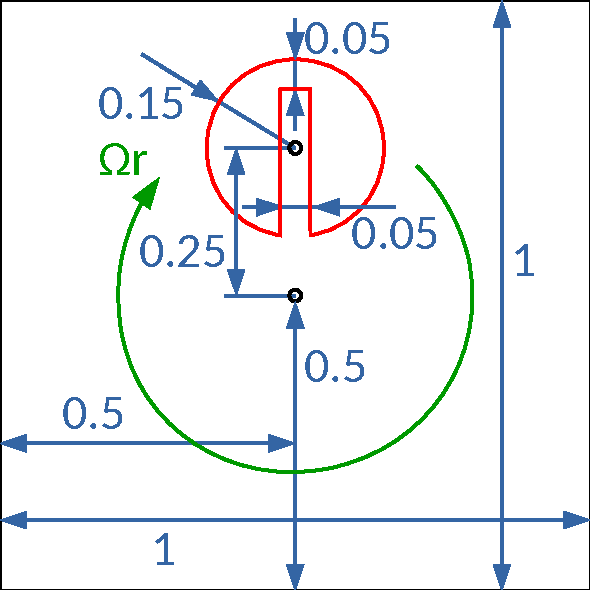
\includegraphics[width=0.95\textwidth]{ZalesakSetup.pdf}
		\caption[Zalesak Setup]{Setup of the Zalesak disk test case.}\label{ZalesakSetup}
	\end{subfigure}%
	\begin{subfigure}{.5\textwidth}
		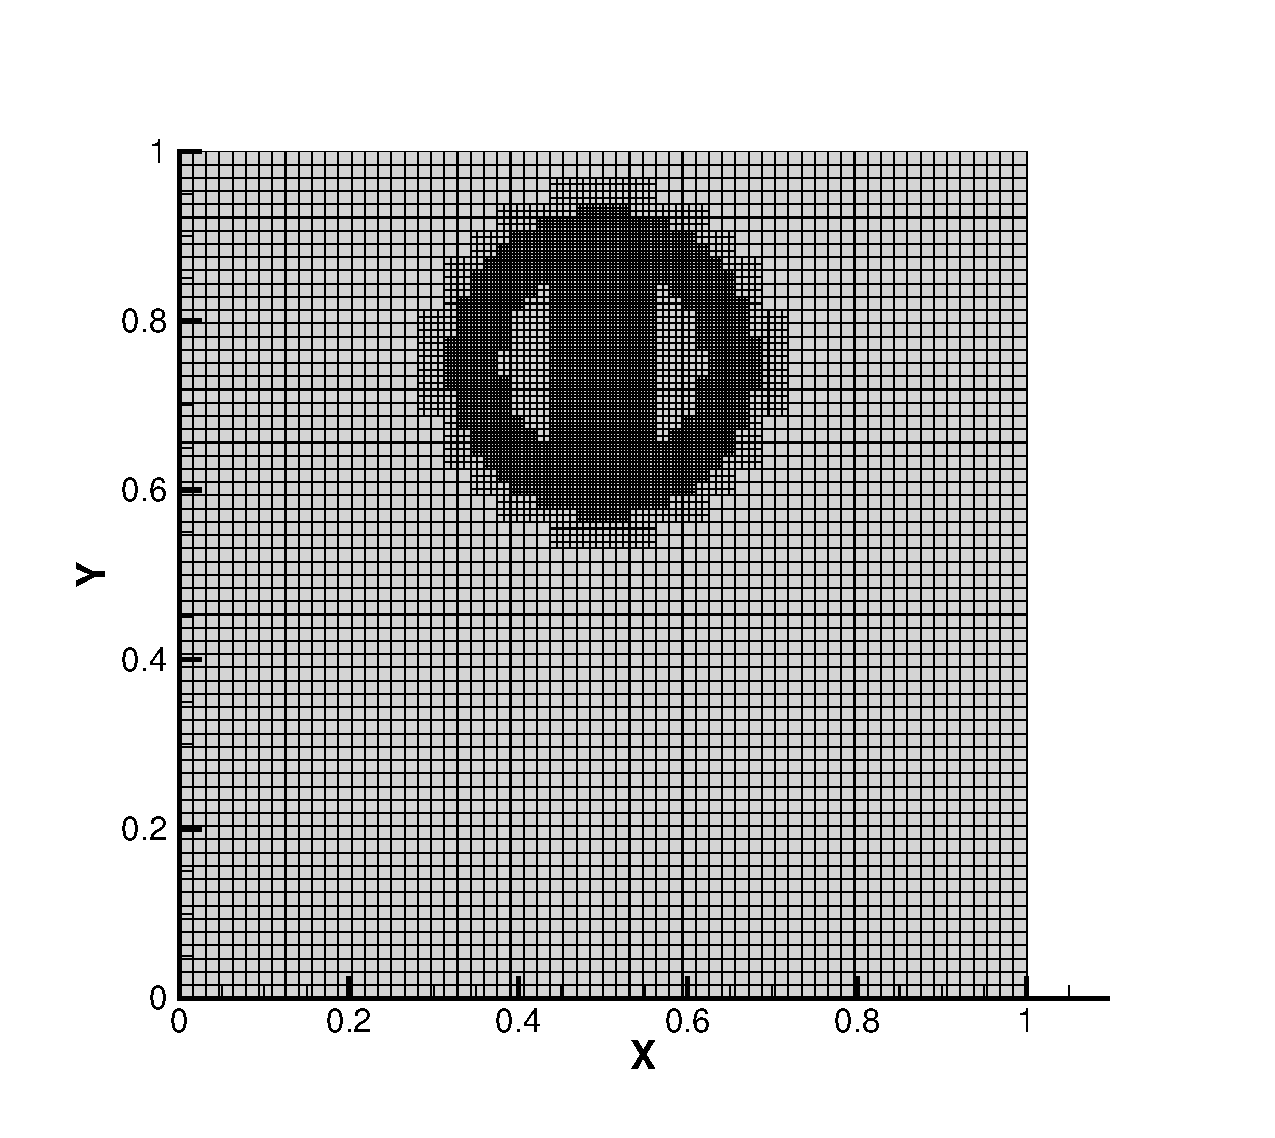
\includegraphics[trim={1.75cm 1.5cm 2.75cm 2.1cm},clip,width=1.1\textwidth]{ZalesakMesh.eps}
		\caption[Zalesak Mesh]{Initial mesh used in Grid-flow.}\label{ZalesakMesh}
	\end{subfigure}
	\caption[Zalesak Disk]{}\label{ZalesakDisk}
\end{figure}\noindent
The purpose of the simulation is to see how distorted the shape of the disk is after a full rotation. The amount of distortion is indicative of the quality of the advection scheme.\par
The velocity field is defined as:
\begin{IEEEeqnarray}{rcccl}\label{ZalesakDiskVelocityField}
	&u&\,=\,&\,-\,&\Omega\left(y-0.5\right)\,,\nonumber\\
	[-0.6\normalbaselineskip]\smash{\left\{\IEEEstrut[6\jot]\right.}&&&\\[-0.6\normalbaselineskip]
	&v&\,=\,&&\Omega\left(x-0.5\right)\,,\nonumber
\end{IEEEeqnarray}
with angular velocity $\Omega=2\pi$. A complete rotation should take one time unit of simulation.\par
\begin{figure}[!ht]
	\centering
	\begin{subfigure}{.5\textwidth}
		\captionsetup{justification=centering}
		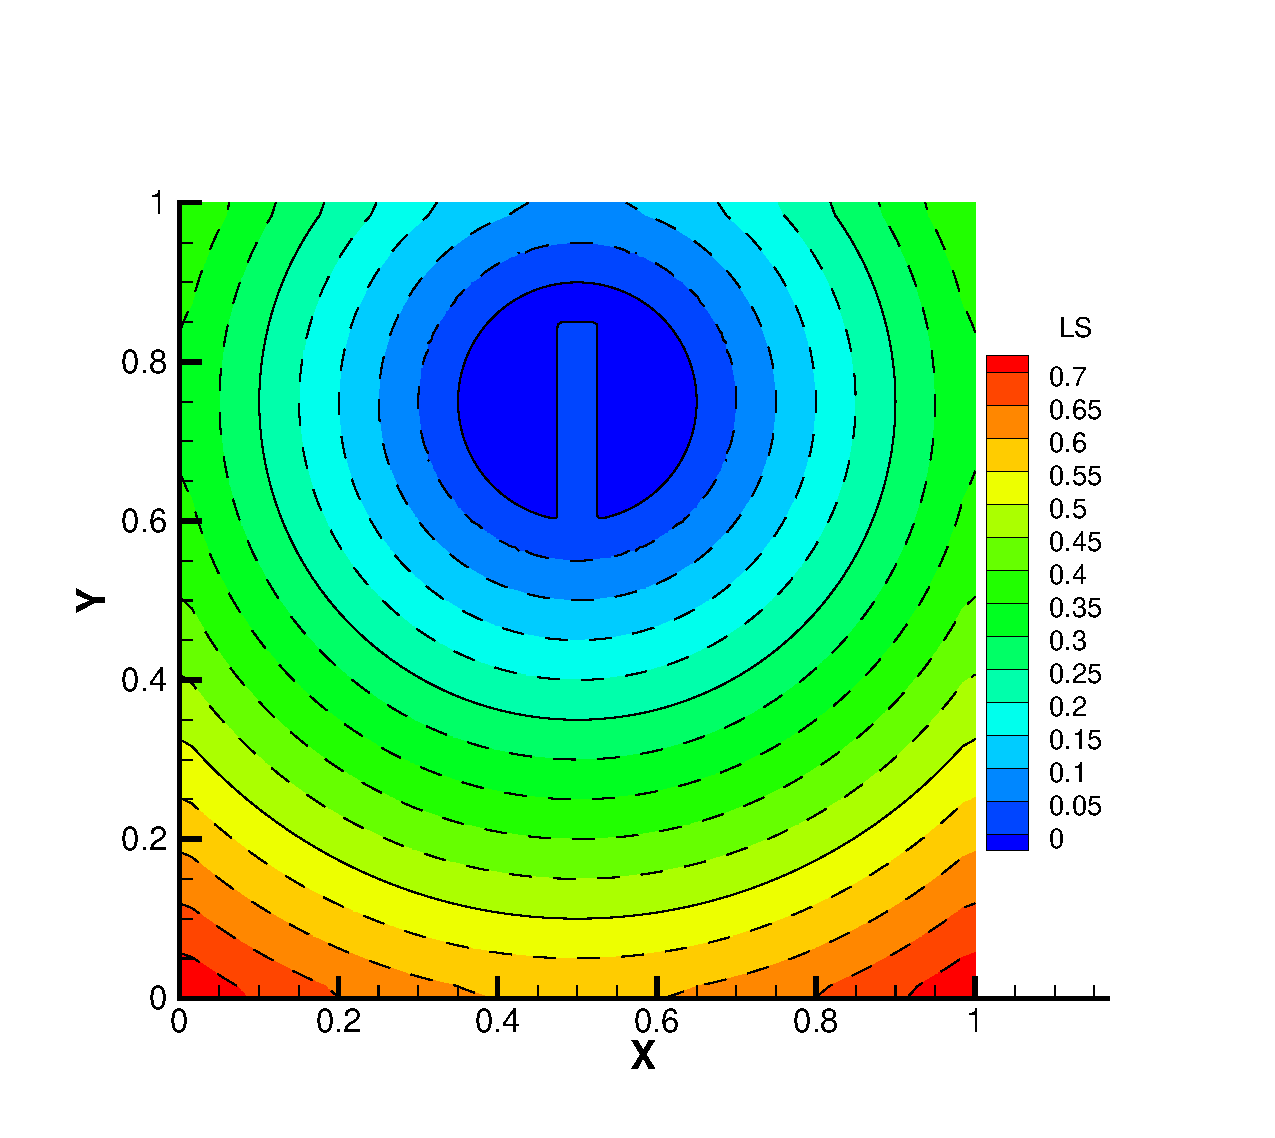
\includegraphics[trim={1.75cm 1.5cm 2.5cm 2.1cm},clip,width=1\textwidth]{ZalesakWC_T0.eps}
		\caption[Zalesak Initial]{Level Set function at the beginning\\of the simulation.}\label{ZalesakInitial}
	\end{subfigure}%
	\begin{subfigure}{.5\textwidth}
		\captionsetup{justification=centering}
		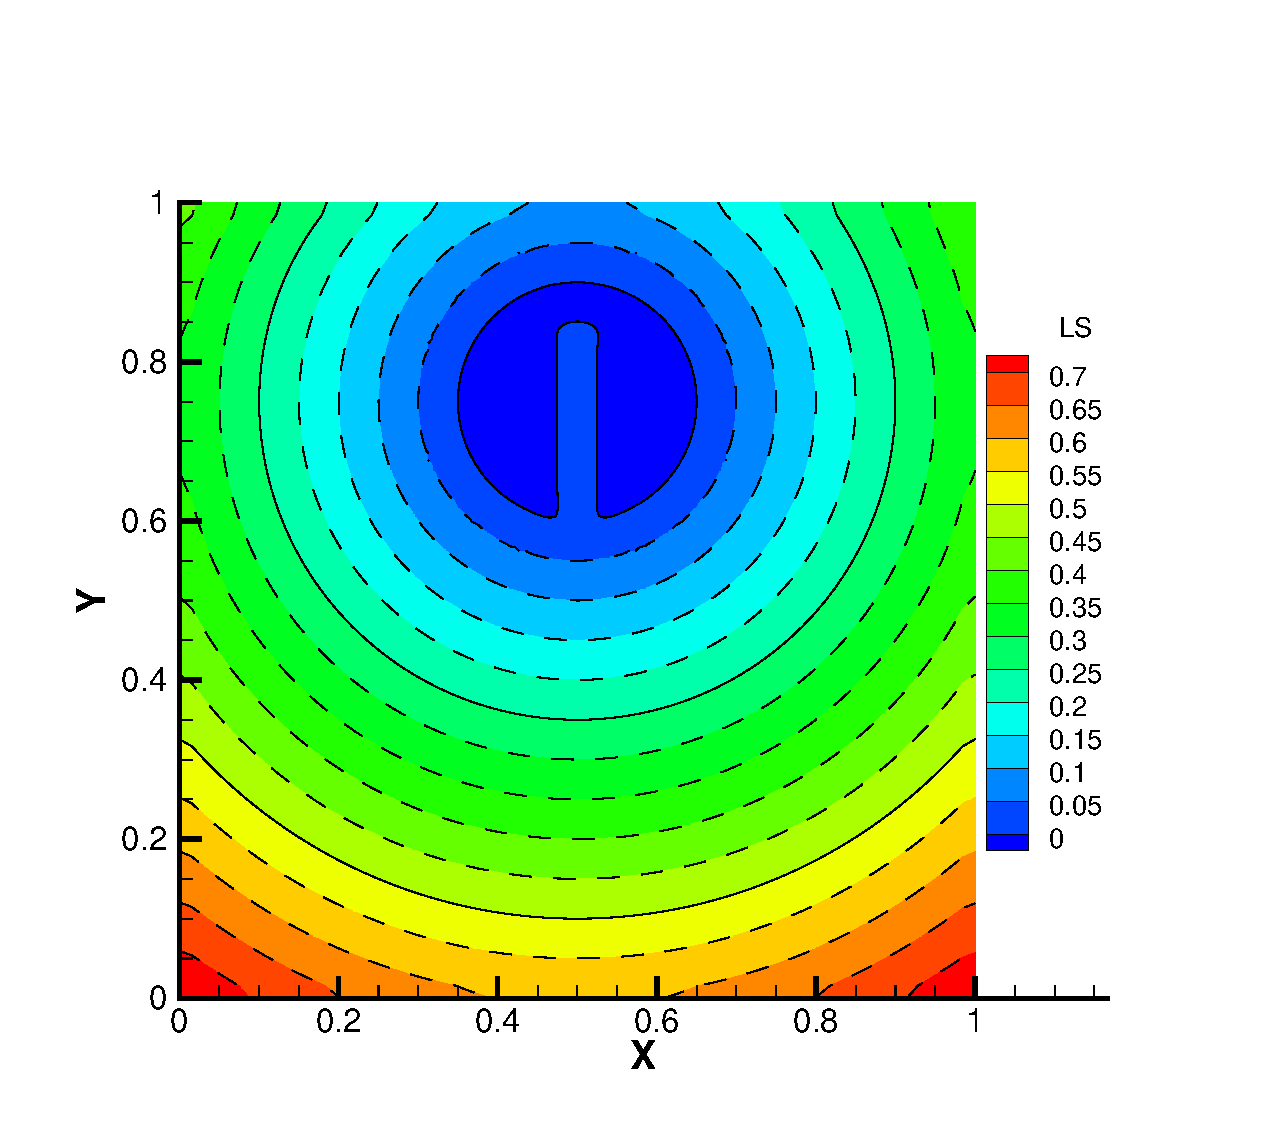
\includegraphics[trim={1.75cm 1.5cm 2.5cm 2.1cm},clip,width=1\textwidth]{ZalesakWC_T1.eps}
		\caption[Zalesak Weakly Compressible]{Level Set function at $t=1$ using the\\weakly-compressible version of the code (WENO).}\label{ZalesakWC_T1}
	\end{subfigure}\\
	\begin{subfigure}{.5\textwidth}
		\captionsetup{justification=centering}
		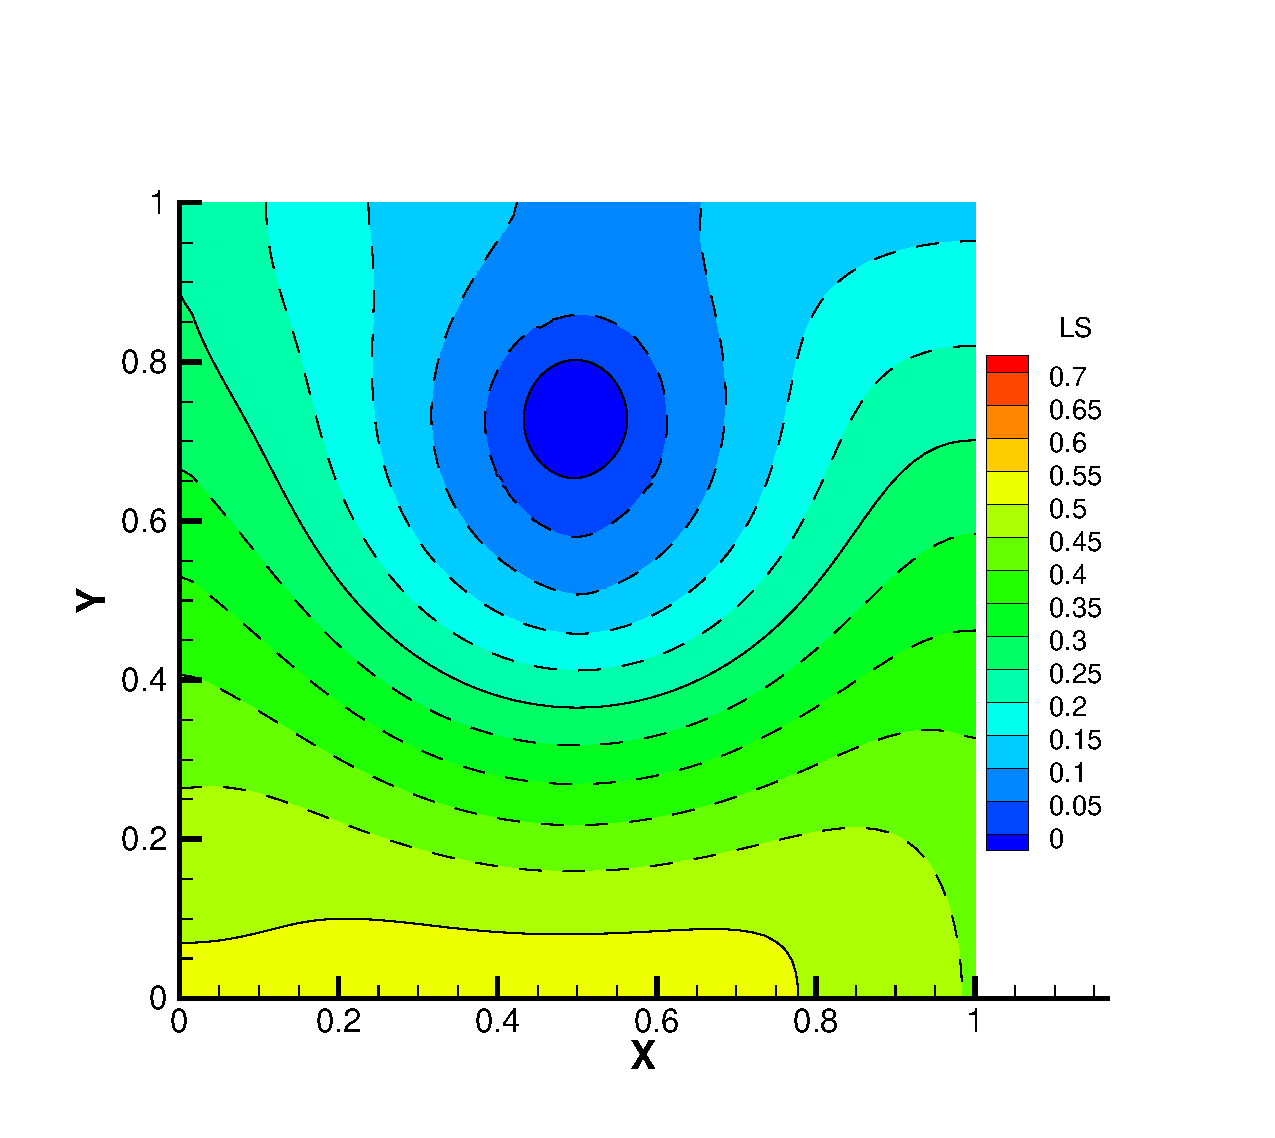
\includegraphics[trim={1.75cm 1.5cm 2.5cm 2.1cm},clip,width=1\textwidth]{ZalesakIC_O_T1.eps}
		\caption[Zalesak Incompressible Old]{Level Set function at $t=1$ using the 2019\\incompressible version of the code (1st order).}\label{ZalesakICO_T1}
	\end{subfigure}%
	\begin{subfigure}{.5\textwidth}
		\captionsetup{justification=centering}
		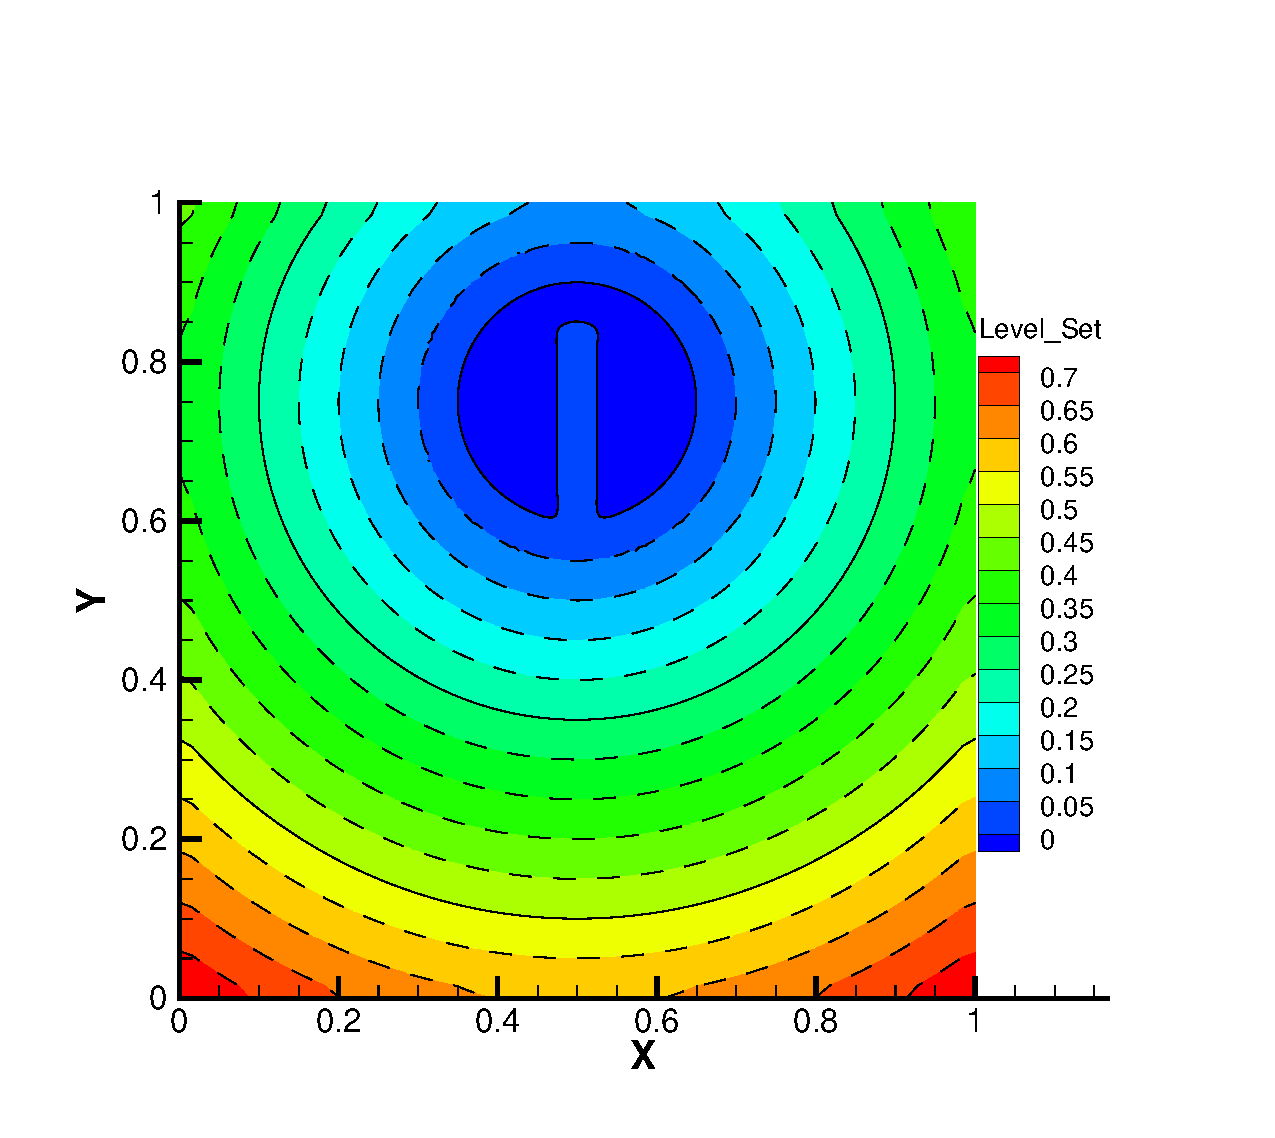
\includegraphics[trim={1.75cm 1.5cm 2.5cm 2.1cm},clip,width=1\textwidth]{ZalesakIC_N_T1.eps}
		\caption[Zalesak Incompressible New]{Level Set function at $t=1$ using the 2020\\incompressible version of the code (WENO).}\label{ZalesakICN_T1}
	\end{subfigure}
	\caption[Zalesak Results]{}\label{ZalesakResults}
\end{figure}\noindent
In Grid-flow, the Level Set function is initialized as the signed distance, negative inside the disk. The time integration of the momentum equation is bypassed so that the velocity field remains equal to \eqref{ZalesakDiskVelocityField} throughout the computation.\par
A dynamically adaptive grid is used, with the highest level of refinement imposed where the absolute value of the level set is close to the minimum grid size, as shown in figure \ref{ZalesakMesh}. The base grid is $64\times 64$ cells ($\Delta x = 1.5625\cdot10^{-2}$) with the finer cells two levels of refinement deeper ($\Delta x = 3.90625\cdot10^{-3}$). During the simulation, the "patch" of finer cells follows the disk around the domain.\par
Figure \ref{ZalesakInitial} shows the Level Set field at the beginning of the simulation. The level curves appear very regular despite the coarseness of the grid far from the disk. This is a product of the post-processing software. However, it can be seen that the sharp angles of the slit are well resolved by the finer cells around the disk.\par
Figures \ref{ZalesakWC_T1} \ref{ZalesakICO_T1} ans \ref{ZalesakICN_T1} show $\phi$ at $t=1$, after a complete rotation. 
They are obtained using, respectively, WENO reconstruction in the weakly-compressible version, a first order accurate reconstruction in the 2019 incompressible version and WENO again, in the 2020 incompressible version. It can be seen that WENO, both in the weakly-compressible and in incompressible formulation preserves well the shape of the disk, albeit blunting the corners of the slit. The first order scheme is instead too diffusive, as the disk almost disappears.
\section{Poisson Equation}\label{Chapter_Results_Poisson Equation}
\subsection{Solver Reinitialization Tests}\label{Subsection_Solver_Reinitialization_Tests}
The multiphase method implemented requires a reinitialization of the PETSc solver at each time iteration (as described in section \ref{Subsection_Reinitialization_of_the_Solver}).\par
\begin{figure}[!ht]
	\centering
	\begin{subfigure}{.5\textwidth}
		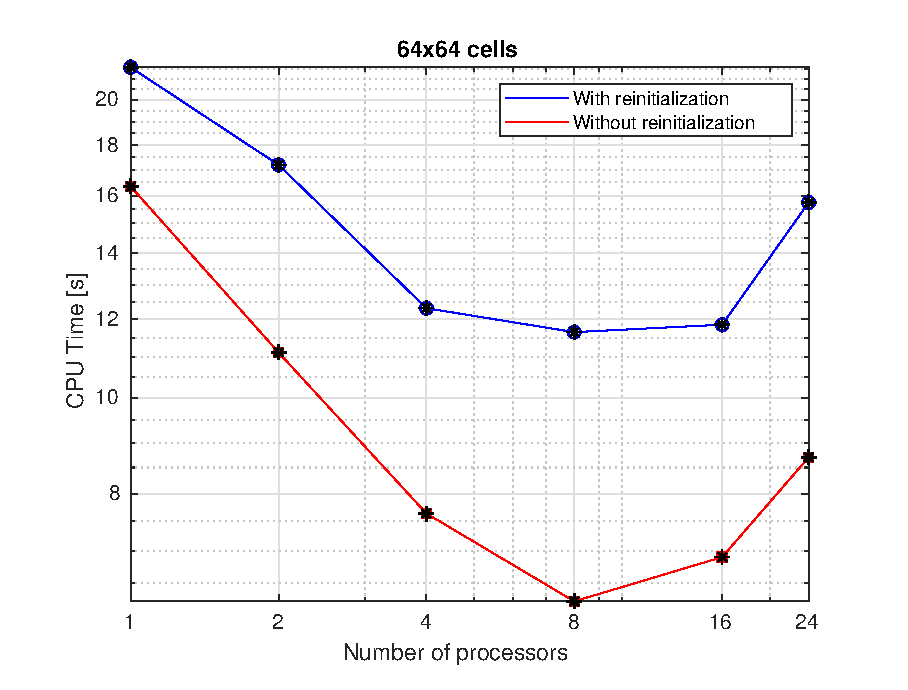
\includegraphics[width=1\textwidth]{CPUTimeTG_64x64.eps}
		\caption[Taylor Green CPU Time 64x64 cells]{}\label{TGCPUTime64x64}
	\end{subfigure}%
	\begin{subfigure}{.5\textwidth}
		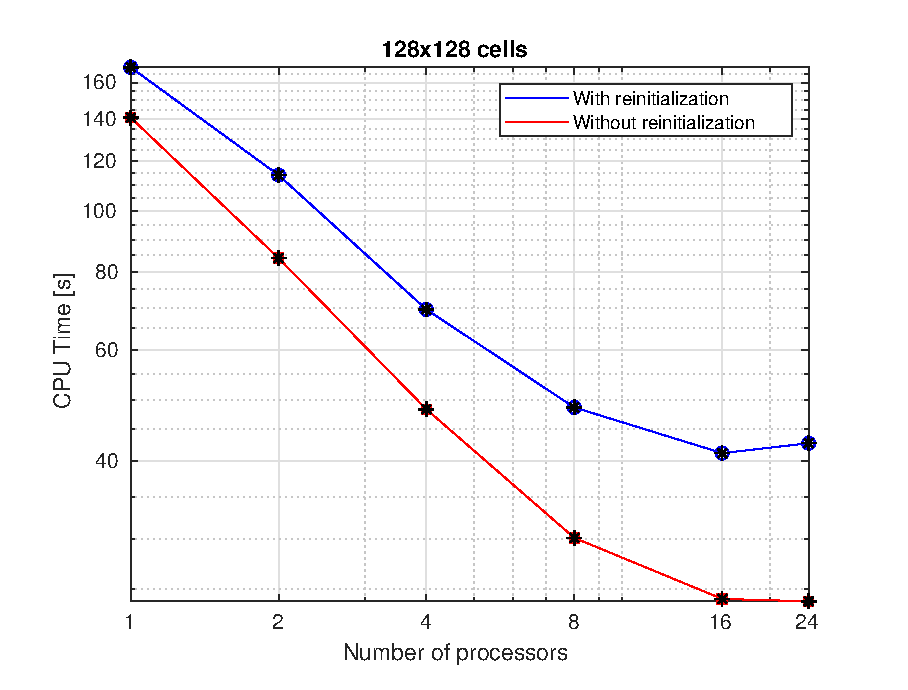
\includegraphics[width=1\textwidth]{CPUTimeTG_128x128.eps}
		\caption[Taylor Green CPU Time 128x128 cells]{}\label{TGCPUTime128x128}
	\end{subfigure}
	\caption[Reinitialization CPU Time cost]{CPU Time for the Taylor-Green vortex test case, with and without reinitialization of the PETSc solver at every time step.}\label{ReinitCPUTimeCost}
\end{figure}\noindent
This operation is bound to slow down the execution of the code to a certain extent. In order to quantify this additional cost, the possibility of forcing the reinitialization of the PETSc solver at every time iteration was added to the base incompressible scheme. The idea is to run the same simulation with and without this forced realization, then compare the CPU times.
The setup chosen for this test is the two-dimensional Taylor-Green vortex, which is initialized as:
\begin{IEEEeqnarray}{rcccl}
	&u\left(x,y\right)&\,=\,&&U_{0}\mathrm{sin}\left(2\pi\dfrac{x}{L}\right)\mathrm{cos}\left(2\pi\dfrac{y}{L}\right)\,,\nonumber\\
	\smash{\left\{\IEEEstrut[13\jot]\right.}&v\left(x,y\right)&\,=\,&-&U_{0}\mathrm{cos}\left(2\pi\dfrac{x}{L}\right)\mathrm{sin}\left(2\pi\dfrac{y}{L}\right)\,,\\
	&p\left(x,y\right)&\,=\,&&\dfrac{\rho U_{0}^2}{4}\left[\mathrm{cos}\left(4\pi\dfrac{x}{L}\right)+\mathrm{cos}\left(4\pi\dfrac{y}{L}\right)\right]\,,\nonumber
\end{IEEEeqnarray}
and advected with no explicit viscosity. The test was run on {\'{E}}cole Centrale's computer cluster \textit{Liger}. A single node was used, constituted by two 12-core Intel Xeon E5-2680v3.\par
Figure \ref{ReinitCPUTimeCost} shows the results. Each point in the graph represents the average over ten simulations. Two grids were used, one made up of $64\times64$ cells, the other of $128\times128$ cells. Different numbers of processors were used: 1, 2, 4, 8, 16 or 24.\par
It can be noted that, not only the reinitialization slows down execution by a tangible amount, but that this effect seems to increase with the number of processors. On the other hand, it should be considered that a test up to 24 processors is not particularly indicative of the scalability of the procedure.\par
Also, both the reinitialized and the non-reinitialized tests start to slow down for an increasing number of processors, hinting that perhaps the grids considered are too small for scalability studies.\par
In the end this test proved inconclusive, and the reinitialization of the solver is in any case unavoidable for a varying density field.
\subsection{Poisson Equation Convergence Tests}\label{Subsection_Poisson_Equation_Convergence_Tests}
\begin{figure}[!ht]
	\centering
	\begin{subfigure}{.5\textwidth}
		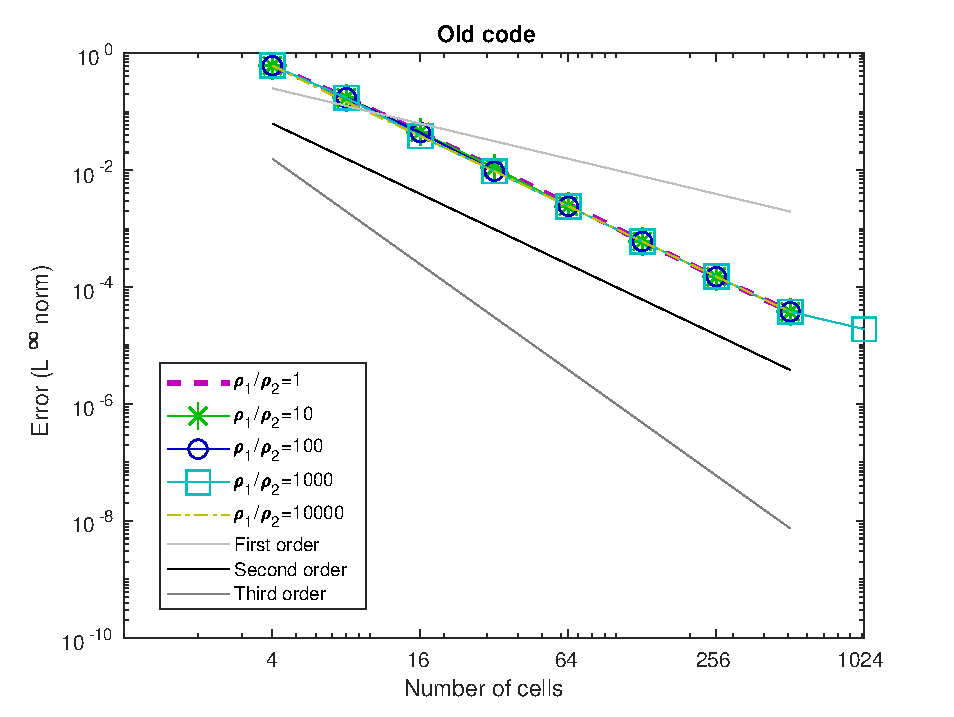
\includegraphics[width=1\textwidth]{PoissonConvergence2019Code.pdf}
		\caption[Poisson Convergence 2019 code]{2019 version of the code.}\label{PoissonTest2019}
	\end{subfigure}%
	\begin{subfigure}{.5\textwidth}
		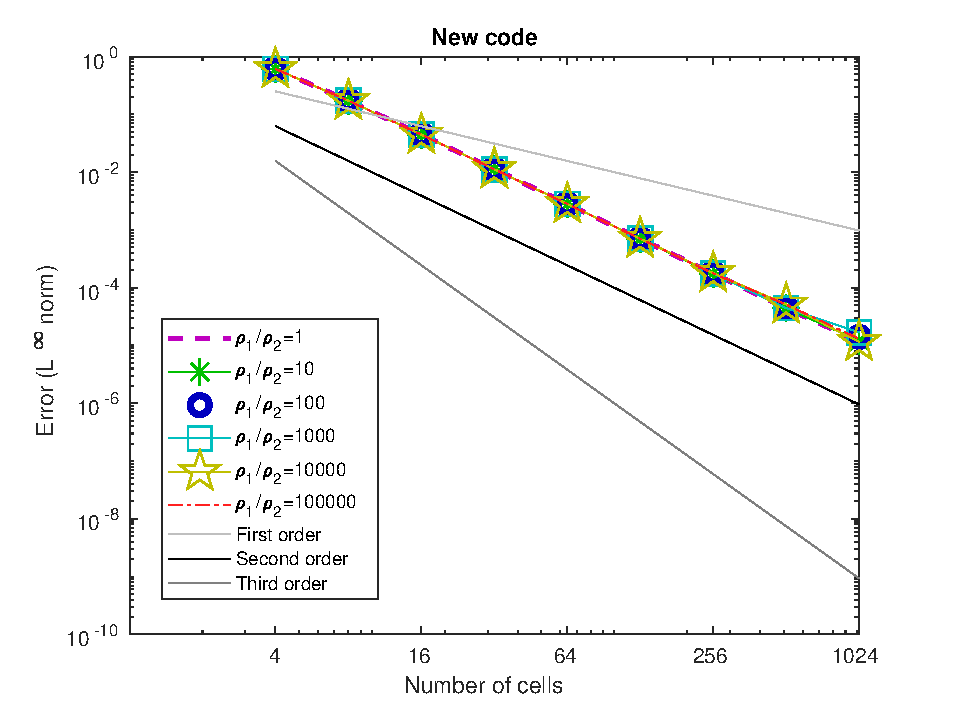
\includegraphics[width=1\textwidth]{PoissonConvergence2020Code.pdf}
		\caption[Poisson Convergence 2020 code]{2020 version of the code.}\label{PoissonTest2020}
	\end{subfigure}
	\caption[Reinitialization CPU Time cost]{$L^{\infty}$ error norm in the solution to the Poisson equation.}\label{PoissonTest}
\end{figure}\noindent
In order to test the implementation of \eqref{LaplacianMatrixVarRho}, a convergence study was devised. For this test, the unit square domain $\left[0,\,1\right]\times\left[0,\,1\right]$ is considered. The upper and lower halves of the domain are filled with different fluids, with the lower one being denser. The velocity field is initialized as
\begin{IEEEeqnarray*}{ccc}
	&u=\dfrac{-2\Delta t\pi\mathrm{sin}\left(2\pi x\right)\mathrm{cos}\left(2\pi y\right)}{\rho\left(x,\,y\right)}\,,\nonumber\\
	[-0.2\normalbaselineskip]\smash{\left\{\IEEEstrut[11\jot]\right.}&\\[-0.2\normalbaselineskip]
	&v=\dfrac{-2\Delta t\pi\mathrm{cos}\left(2\pi x\right)\mathrm{sin}\left(2\pi y\right)}{\rho\left(x,\,y\right)}\,.\nonumber
\end{IEEEeqnarray*}
This is analogous to the Taylor-Green vortex, except for the variable density. For this test, the advection and source terms of the momentum equation are bypassed and only one time step executed. This means that, at the end of this single time step, the solution to the pressure Poisson equation \eqref{ChorinMulti_04} is:
\begin{equation*}
	p=\mathrm{cos}\left(2\pi x\right)\mathrm{cos}\left(2\pi y\right)\,.
\end{equation*}
This expression can be used to quantify the error in the solution. Figure \ref{PoissonTest} shows the error in the $L^{\infty}$ norm for various mesh sizes and different density ratios between the lower and upper portions of the domain.\par
It can be seen that the operators used for solving equation \eqref{ChorinMulti_04} are second order accurate, even with a variable density.
\section{Multiphase Flow Tests}\label{Chapter_Results_Multiphase_Flow_Tests}
\subsection{Hydrostatic Test Case}\label{Section_Hydrostatic_Test_Case}
The setup of this test case is similar to the one descibed previously (\ref{Subsection_Poisson_Equation_Convergence_Tests}): a square domain is considered, the top half is filled by one fluid, the bottom by a second fluid 1000 times denser. The two fluids are subject to the effects of gravity, in the form of a constant source term added to the momentum equation, pulling downward. The boundary conditions are free-slip, due to the absence of viscosity). The velocity is initially null.\par
Ideally no fluid movement should arise during the computation.
\begin{figure}[!ht]
	\centering
	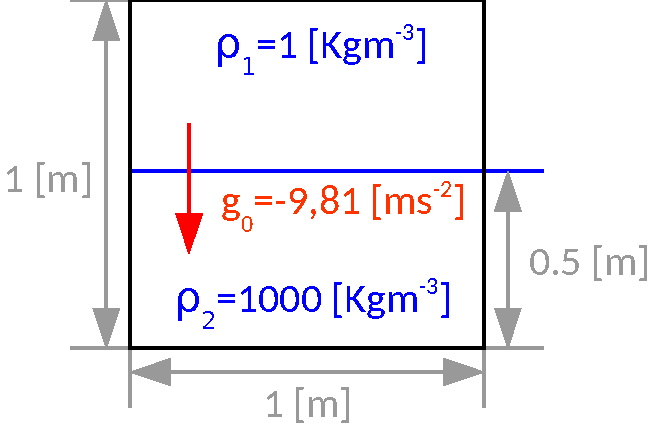
\includegraphics[width=0.4\textwidth]{Hydrostatic_setup.pdf}
	\caption[Hydrostatic Test Case Setup]{Initial setup of the hydrostatic test case.}\label{HydrostaticSetup}
\end{figure}\noindent
This is found to be the case if the difference in density between the two fluids is removed, or if the density update \eqref{ChorinMulti_03} is turned off. Applying the full multiphase scheme \eqref{ChorinMulti}, oscillations start to originate at the interface between the two fluids.\par
\begin{figure}[!ht]
	\centering
	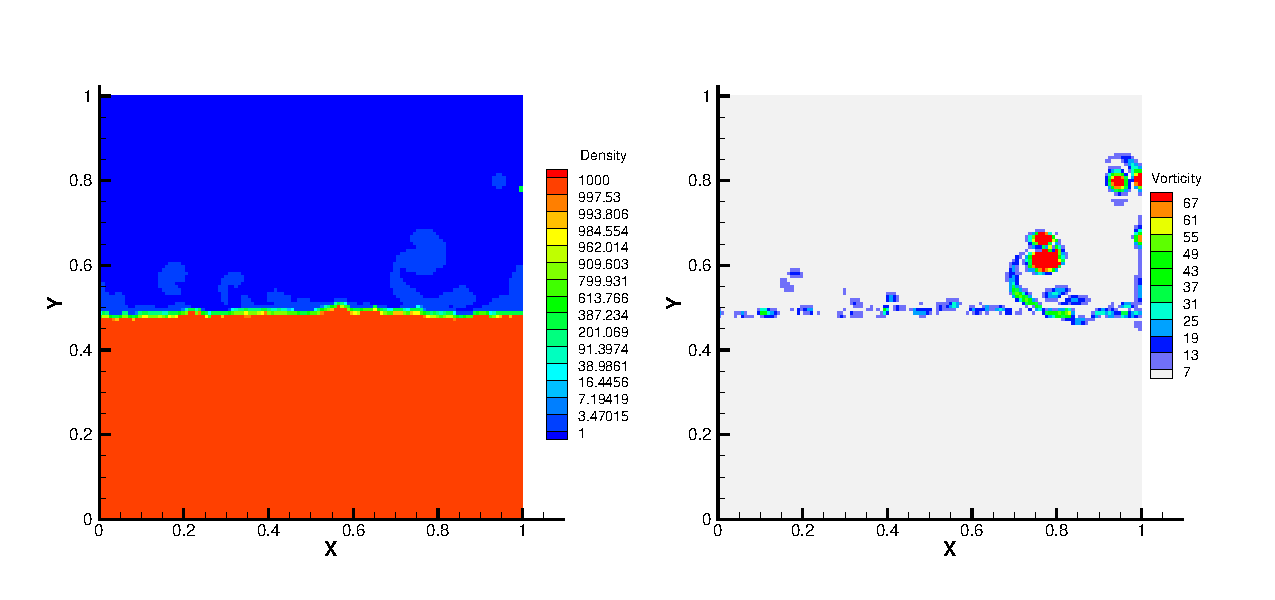
\includegraphics[width=1.1\textwidth]{HydrostaticT6p83.eps}
	\caption[Hydrostatic Test Density Viscosity]{The density and the vorticity field at $t = 6.83 [s]$.}\label{HydrostaticT6p83}
\end{figure}\noindent
Figure \ref{HydrostaticT6p83} was obtained on a $128\times128$ uniform static grid, using WENO for flux reconstruction and forward Euler for time integration. It shows, after $6.83$ seconds of simulation time, how the oscillations ripple the interface between the two fluids, shedding vortices in the lighter one.\par
Figure \ref{HydrostaticTime} shows how the oscillations evolve in time by plotting the magnitude of the maximum velocity in semi-logarithmic scale. This data was obtained on a $32\times32$ grid. Time integration is, again, forward Euler. The graph on the left is obtained using a WENO reconstruction for both the Level Set and the velocity, while graph on the right using WENO for the velocity and MUSCL for the Level-Set. In both cases, at the beginnig the oscillations grow exponentially, then, their amplitude "stabilizes". The WENO -WENO simulation, at $t\approx 11\,[s]$, starts growing again and crashes, while the MUSCL - WENO one is still running at $t=12\,[s]$.\par
\begin{figure}[!ht]
	\centering
	\begin{subfigure}{.5\textwidth}
		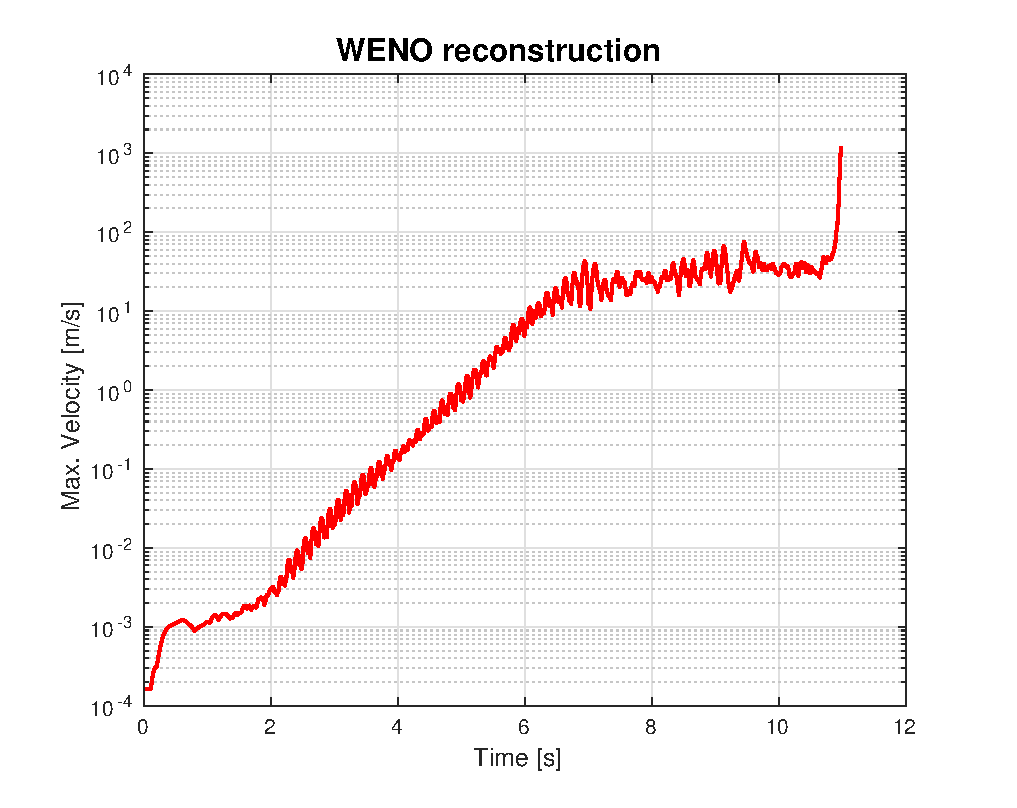
\includegraphics[width=1\textwidth]{Hydrostatic_WENOTime.eps}
		\caption[Hydrostatic ]{}\label{HydrostaticTimeWENO}
	\end{subfigure}%
	\begin{subfigure}{.5\textwidth}
		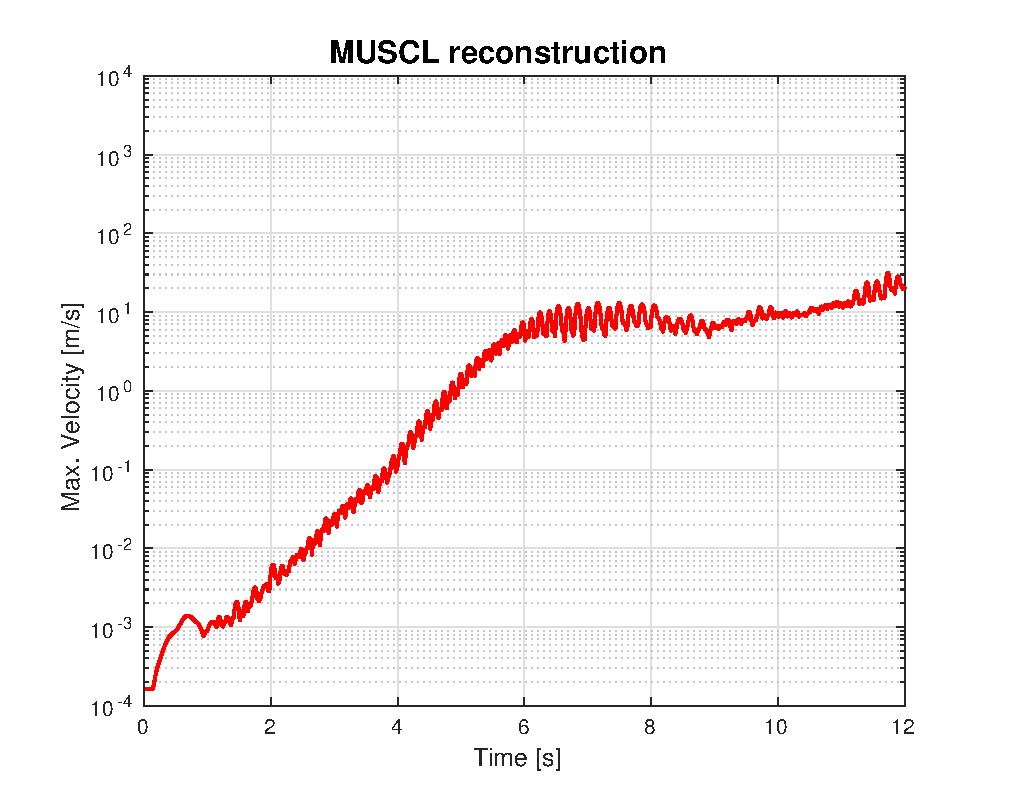
\includegraphics[width=1\textwidth]{Hydrostatic_MUSCLTime.eps}
		\caption[Poisson Convergence 2020 code]{}\label{HydrostaticTimeMUSCL}
	\end{subfigure}
	\caption[Poisson equation convergence study]{Maximum velocity in semi-logarithmic scale versus simulation time for the hydrostatic test case.}\label{HydrostaticTime}
\end{figure}\noindent
Many factors influence the growth rate of the oscillations and their final amplitude. Integration with the fourth order Runge-Kutta scheme, as opposed to forward Euler, reduces their amplitude considerably, and so does decreasing the tolerance of the GMRES solver, which is set by default to $10^{-5}$ by PETSc. This hints that the main source of these oscillations may be the imperfect solution to the pressure Poisson equation. In general, higher order spatial discretization schemes affect stability negatively, with the worst results obtained using WENO with no smoothness indicators.\par
The maximum time step presented in section \ref{Subsection_Time_Step} is, in general, valid only at the beginning of the simulation, since at some point the oscillations reach enough magnitude for $\Delta t_{h}$ to be higher than $\Delta t_{max}$. This initial phase, however, affects the whole simulation: lower values of $\Delta t_{max}$ slow down the onset of instability.\par
Another aspect whose effect on stability was investigated is the span of the Heaviside function \eqref{DeltaFunctionIBM} used to regularize the density field, determined through the parameter $\alpha$. While imposing a sudden jump (very high $\alpha$) in density proved, as expected, detrimental to stability, a correlation between the span and the onset of oscillations could not be found.\par
For the hydrostatic case described above, there is one way to avoid oscillations entirely, which is to use the incremental version of the projection scheme. Unfortunately, this is only due to the fact that, if the initial pressure field is chosen accurately enough to balance the effects of gravity, the right-hand side of the pressure equation is always null. This is useless as it does not address the source of the oscillations, but simply bypasses the numerical scheme altogether.\par
The incremental formulation did not provide advantages in terms of stability in more dynamic computations, such as the dambreak.\par
By choosing carefully the factors listed above, one can set up a simulation in which oscillations grow slowly enough and are sufficiently low in amplitude, at least for a static or slowly moving interface.
\subsection{Linear Sloshing}\label{Section_Linear_Sloshing}
\begin{figure}[!ht]
	\centering
	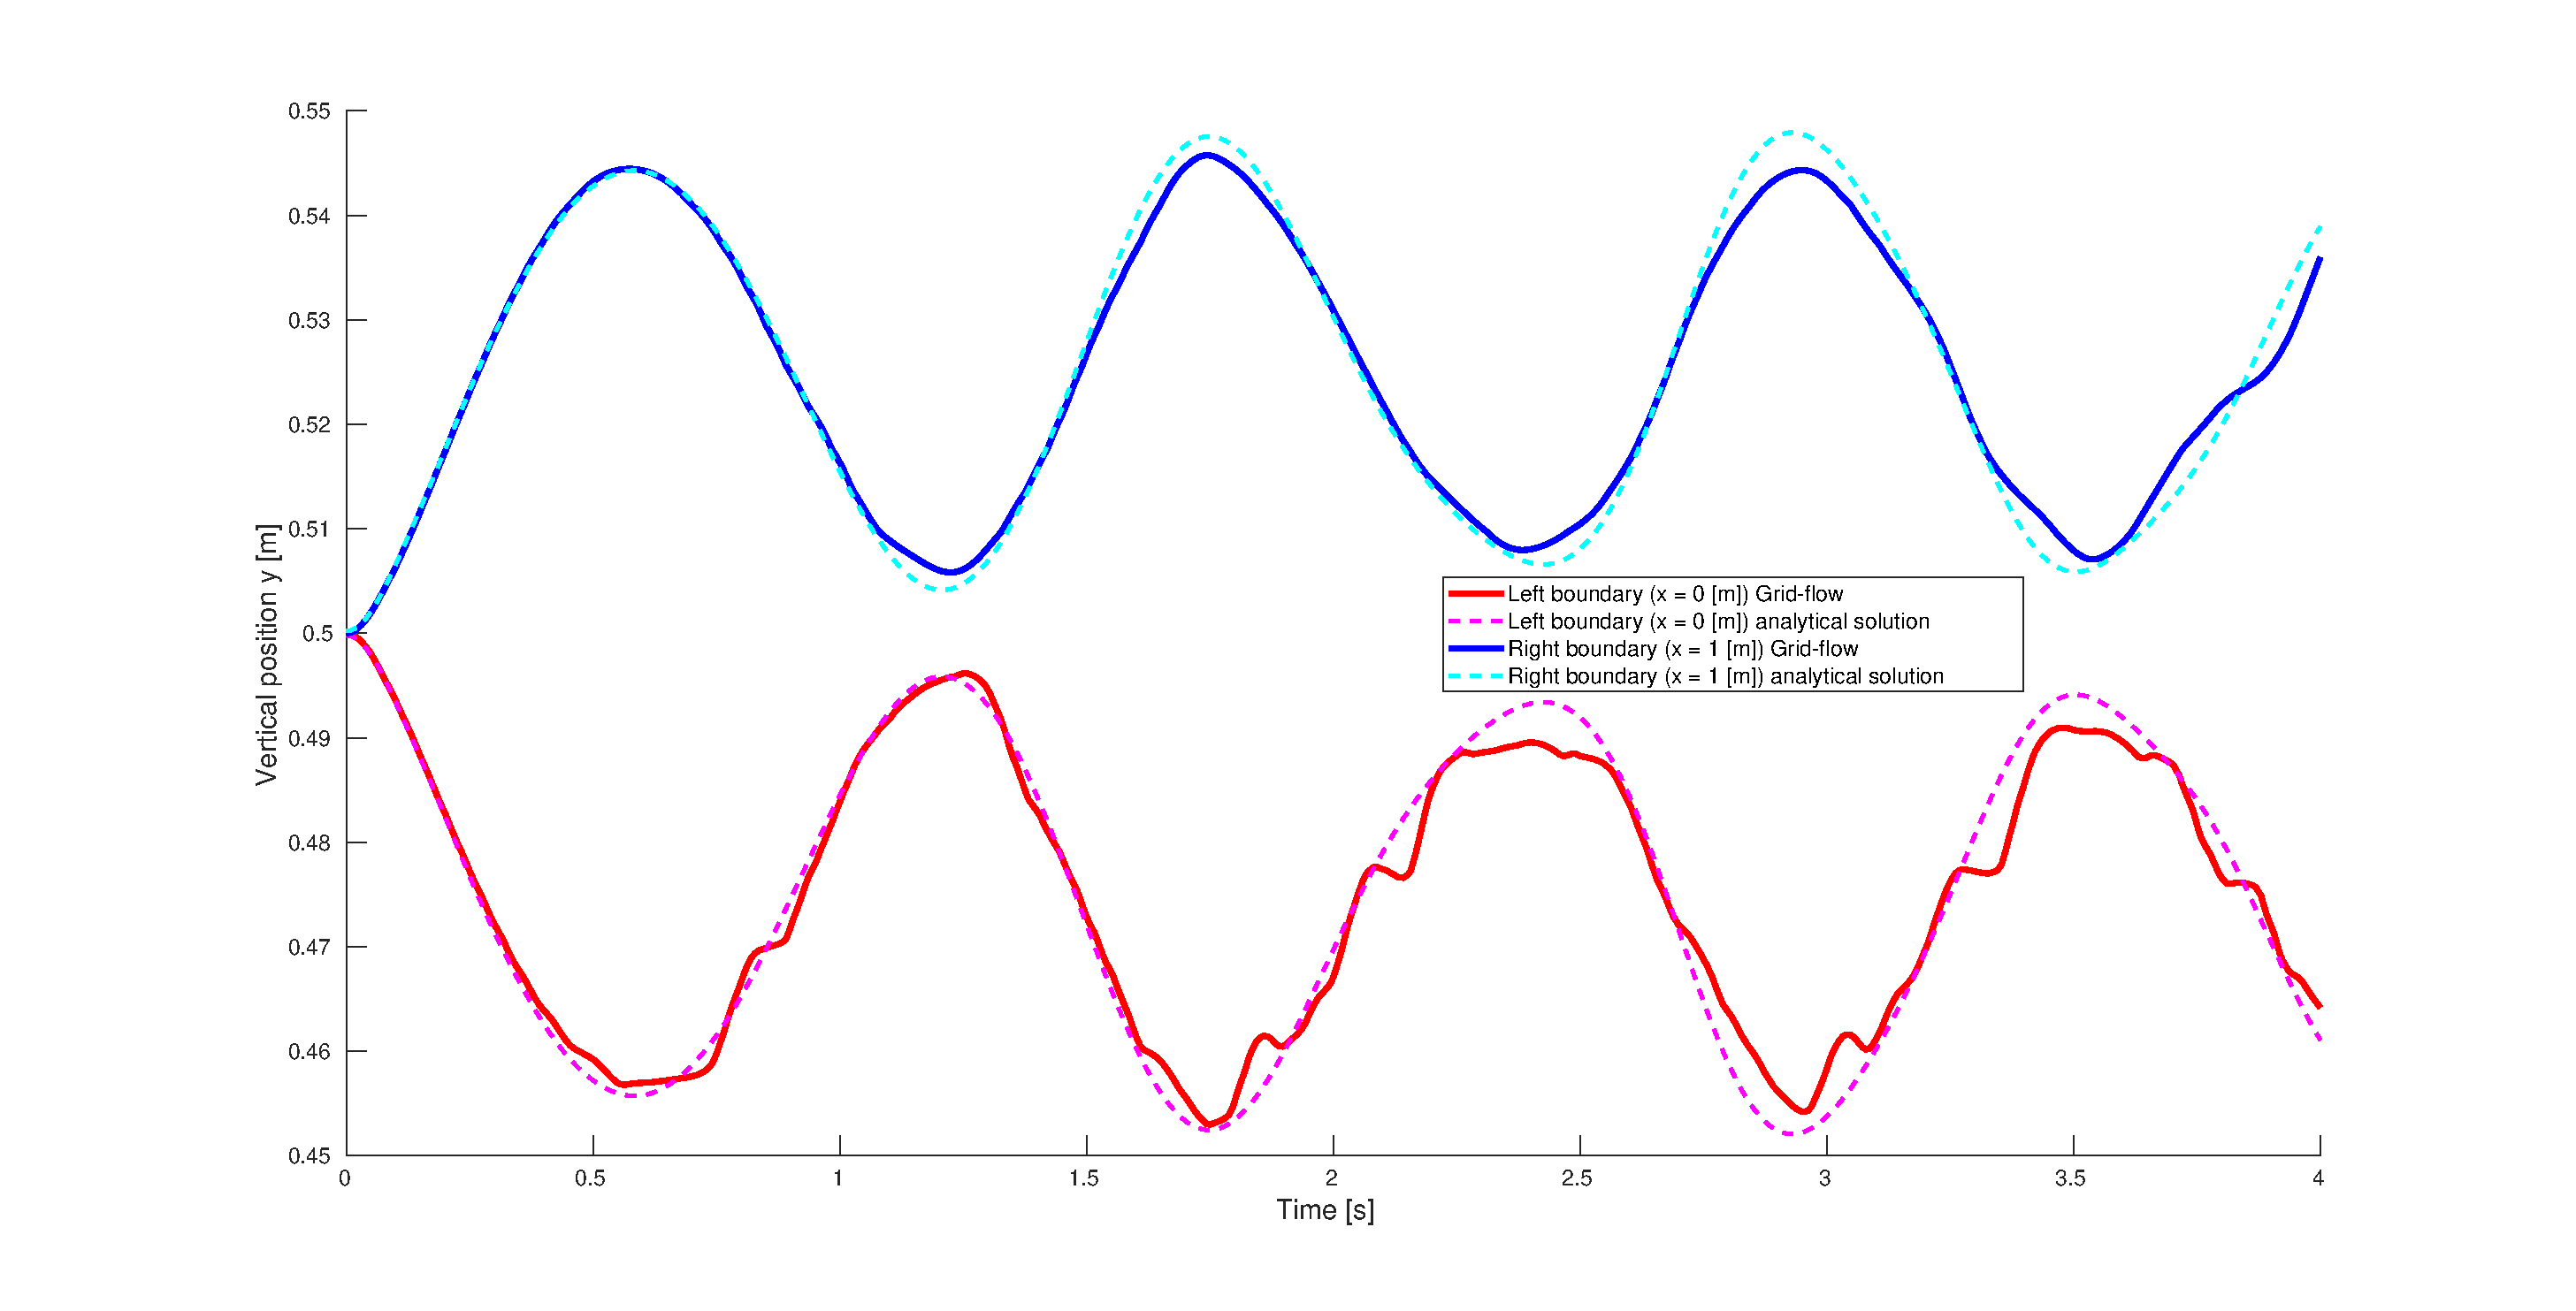
\includegraphics[width=0.9\textwidth]{LinearSloshingInterfaceMovement.eps}
	\caption[Linear Sloshing, interface vs. time]{The temporal evolution of the vertical position of the interface at the left and right extremes of the domain.}\label{LinearSloshingTime}
\end{figure}\noindent
The linear sloshing test case has a setup similar to the hydrostatic one, but with the addition of a small horizontal acceleration. This means that the equilibrium position for the interface between the two fluids is slightly inclined, compared to the initial horizontal one.
During the simulation, the extremes of the interface start to oscillate up and down. Ideally, in the absence of viscosity, this oscillation would continue indefinitely.\par
\begin{figure}[!ht]
	\centering
	\includegraphics[width=1.1\textwidth]{LinearSloshingT4.eps}
	\caption[Linear Sloshing, t=4]{Level Set and density fields at $t=4\,[s]$.}\label{LinearSloshingT4}
\end{figure}\noindent
The simulation is run on the same square domain used for the hydrostatic test, using a $256\times256$ cells static grid, $\Delta t_{max}=2^{-7}\,[s]$, WENO for advecting both the velocity and the Level Set, and fourth order Runge-Kutta for time integration. Four seconds of simulation are computed.\par
An analytical solution for the movement of the interface can be derived from linearized potential theory:
\begin{IEEEeqnarray}{l}
	k_{n}=\dfrac{n\pi}{L}\,,\nonumber\\\
	\omega_{n}^{2}=\dfrac{g_{0}k_{n}\left(\rho_{2}-\rho_{1}\right)}{\rho_{1}\mathrm{coth}\left(\omega_{2n+1}t\right)+\rho_{2}\mathrm{coth}\left(k_{2n+1}x\right)}\,,\label{LinearSlowhingAnalytical}\\
	y\left(x,\,t\right)=h_{2}+\dfrac{a}{g_{0}}\left[x-\dfrac{L}{2}+\sum_{n=0}^{\infty}\dfrac{4}{Lk_{2n+1}^{2}}\mathrm{cos}\left(\omega_{2n+1}t\right)\mathrm{cos}\left(k_{2n+1}x\right)\right]\,,\nonumber
\end{IEEEeqnarray}
where $a$ is the horizontal acceleration, $h_{1}$ and $h_{2}$ the heights of the upper and lower portions of the domain occupied by the two fluids, and $L$ the horizontal size of the domain. The validity of \eqref{LinearSlowhingAnalytical}, as reported in \cite{Bardin2015}, is limited to low ratios between the horizontal and vertical accelerations ($a / g_{0}\ll 1$). The value of $a$ usually found in the literature \cite{Bardin2015}\cite{Grenier2013} is $0.01$, while for this test a value of $0.5$ is used. The shape of the domain also differs, as the one more commonly used is skewed in the $y$ direction, however, as shown in figure \ref{LinearSloshingTime}, the results of the simulation do not deviate excessively from the theoretical values.\par
While no crash occurs during this time, and the behaviour of the interface is relatively close to the expected one, it is clear from figure \ref{LinearSloshingT4} that the oscillations seen in the hydrostatic test have started developing.
\subsection{Dambreak (2019)}\label{Section_Dambreak_2019}
The dambreak test consists in having a pocket of denser fluid on one side of the domain which, when the simulation starts, floods the other side of the domain.\par
\begin{figure}[!ht]
	\centering
	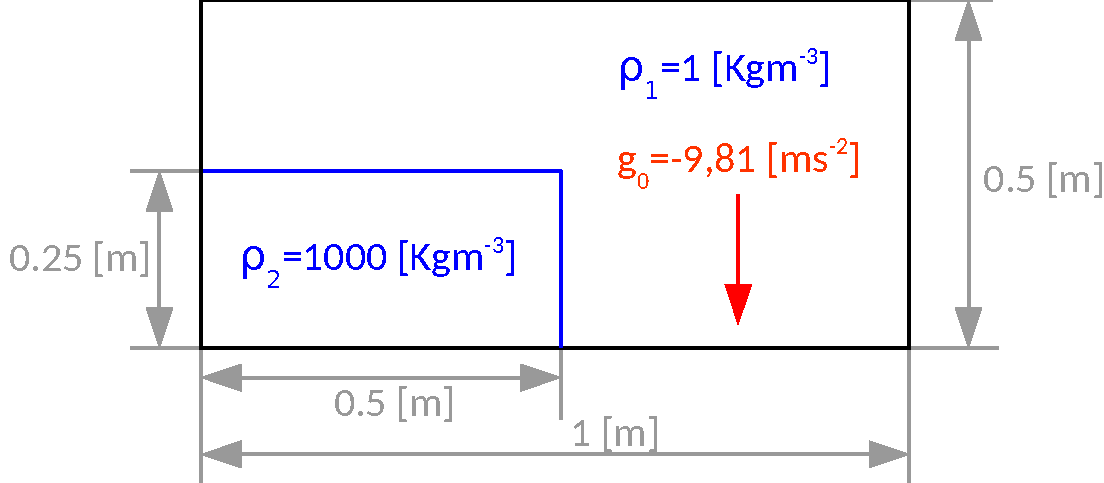
\includegraphics[width=0.6\textwidth]{Dambreak_setup.pdf}
	\caption[Dambreak Test Setup]{Initial setup of the Dambreak test.}\label{DambreakSetup}
\end{figure}\noindent
The domain used for this test is a rectangle ($\left[0,\,1\right]\times\left[0,\,0.5\right]$), as shown in figure \ref{DambreakSetup}. This and the following tests are intended only as studies of the stability properties of the scheme.\par
\begin{figure}[!ht]
	\centering
	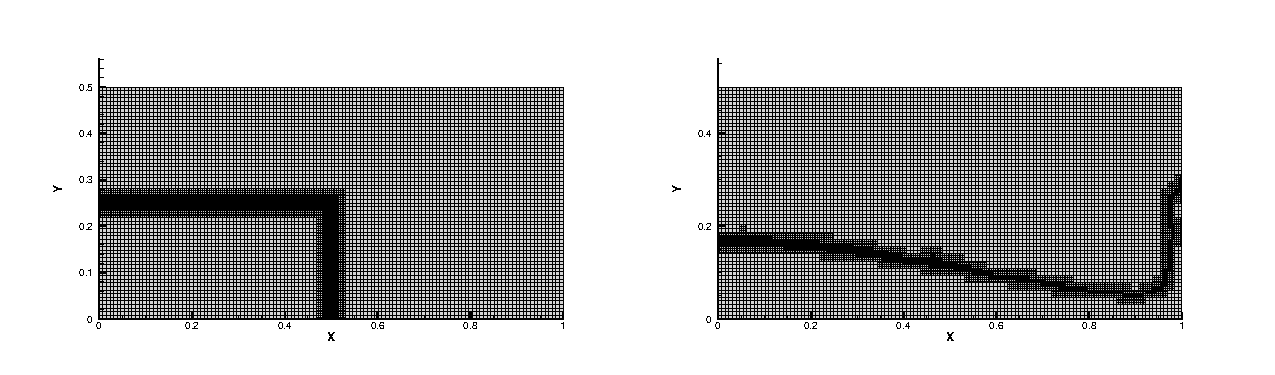
\includegraphics[width=1\textwidth]{DambreakAMRMesh.eps}
	\caption[Dambreak AMR Grid]{The dynamically adaptive grid at $t = 0\,[s]$ (left) and at $t = 0.5\,[s]$ (right) for the 2019 test.}\label{Dambreak2019Grid}
\end{figure}\noindent
This test was first run on the earlier (2019) implementation of the scheme, with the velocity fluxes reconstruted using WENO and the level Set fluxes using the first order scheme. For this first simulation, dynamic adaptive refinement is used, with the same Level-Set-based refinement criterion used for the Zalesak disk. The base grid is made of $128\times 64$ cells ($\Delta x = 7.8125\cdot 10^{-3}\,[m]$), the finer cells are two levels of refinement deeper ($\Delta x = 1.953125\cdot 10^{-3}\,[m]$). $\Delta t_{max} = 0.01 [s]$ and the simulation is run for 25 seconds.\par
\begin{figure}[!ht]
	\centering
	\includegraphics[width=1.1\textwidth]{Dambreak2019Times.eps}
	\caption[Dambreak AMR 2019]{The two fluids at various times in the dambreak simulation run on the 2019 code.}\label{Dambreak2019Times}
\end{figure}\noindent
\begin{figure}[!ht]
	\centering
	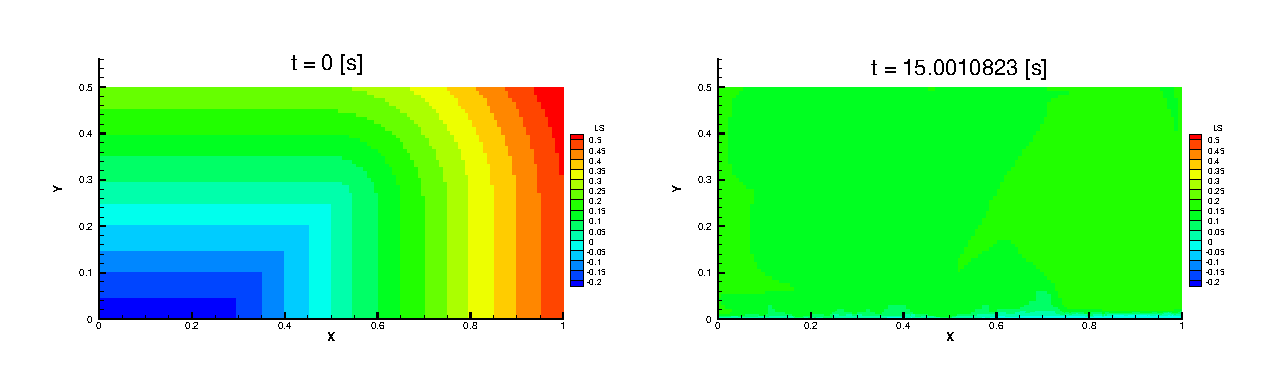
\includegraphics[width=1.1\textwidth]{Dambreak2019LS.eps}
	\caption[Dambreak 2019 Level Set Diffusion]{The Level Set field at two different times in the dambreak simulation run on the 2019 code. In the second one the denser fluid has almost entirely disappeared due to diffusion.}\label{Dambreak2019LS}
\end{figure}\noindent
No crash is encountered, and the oscillations observed in the hydrostatic and linear sloshing tests are not evident. On the downside, the denser fluid loses mass to the lighter one and disappears completely after $t\approx 18\,[s]$. This is due to the excessive diffusion of the advection scheme used for the Level Set. It can be observed in figure \ref{Dambreak2019LS} that the Level Set field is almost entirely uniform by the end of the simulation.\par
\begin{figure}[!ht]
	\centering
	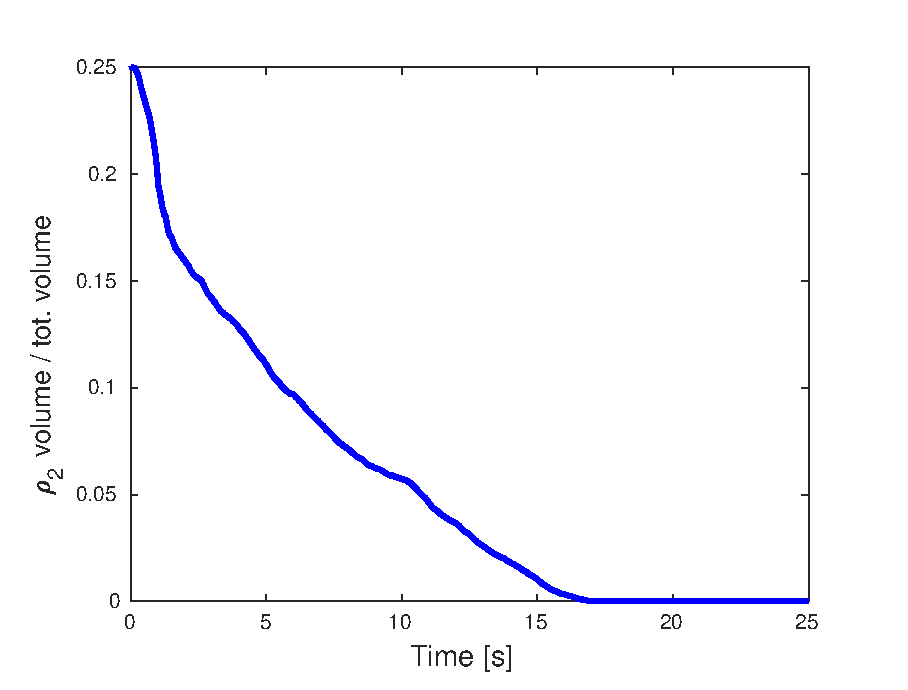
\includegraphics[width=0.6\textwidth]{DambreakVolumeDecrease2019.eps}
	\caption[Dambreak 2019 Denser fluid volume vs. time]{Fraction of the domain volume occupied by the denser fluid as a function of time. Simulation run on the 2019 version of the code.}\label{DambreakVolumeDecrease2019}
\end{figure}\noindent
Further tests revealed that this setup may suffer from stability problems as well. While for carefully chosen parameters the computation runs smoothly until the chosen 25 seconds limit, in other situations the velocity starts to grow exponentially, and the simulation is run to a halt due to \eqref{HyperbolicTimeStep}.\par
It was, unfortunately, not possible to identify a precise trend in the choice of parameters more conductive to stability. As observed in section \ref{Section_Hydrostatic_Test_Case} for the hydrostatic test, a lower $\Delta t_{max}$ seems to aid stability, however, lowering it below a certain point is actually detrimental.\par
The effects of the span of the Heaviside function were investigated, with spans as wide as 9 cells considered. Again, a correlation with the stability of the simulation was not found. All results reported here were obtained setting $\alpha=3$, which is the default value for \eqref{DeltaFunctionIBM} when applied to the immersed boundary. This corresponds to a span of about 2-3 cells.
\subsection{Dambreak (2020)}\label{Section_Dambreak_2020}
After the upgrade to the 2020 version of the code, both WENO and MUSCL reconstruction schemes were available for advection. It was decided to test four possible combinations of reconstruction schemes:
\begin{itemize}
	\item Velocity reconstructed with WENO, Level-Set reconstructed with WENO.
	\item Velocity reconstructed with WENO, Level-Set reconstructed with MUSCL.
	\item Velocity reconstructed with MUSCL, Level-Set reconstructed with WENO.
	\item Velocity reconstructed with MUSCL, Level-Set reconstructed with MUSCL.
\end{itemize}
For these tests, the dynamically refined grid was abandoned in favour of a static $256\times128$ ($\Delta x = 3.90625\cdot 10^{-3}\,[m]$) grid, and the time limit was set to $10$ rather than $25$ seconds. The setup of the test shown in figure \ref{DambreakSetup} is otherwise unaltered. The evolution in time of the density field is shown in figures \ref{Dambreak4Tests_1}, \ref{Dambreak4Tests_2}, \ref{Dambreak4Tests_3}, \ref{Dambreak4Tests_4}, \ref{Dambreak4Tests_5}, \ref{Dambreak4Tests_6}, \ref{Dambreak4Tests_7} and \ref{Dambreak4Tests_8}.
\subsubsection{Velocity reconstructed with WENO, Level-Set reconstructed with WENO}
This combination was the least successful. Every attempt crashed between $0.3$ and $0.4$ seconds of simulation time, before the front of denser fluid reaches the right boundary. Attempts were made with and without the WENO smoothness indicators. When active, the crash is delayed by no more than $0.1$ seconds.
\subsubsection{Velocity reconstructed with WENO, Level-Set reconstructed with MUSCL}
This setup behaved similarly to the 2019 code, with the simulation not crashing and the denser fluid progressively disappearing due to the diffusion of the advection scheme used for the Level Set. It can be noted that no denser fluid remains at the $10$-second mark, hence diffusion is actually faster. This could be explained by the fact that, while the base grid used for the 2019 test was coarser than the one used for this test, the cells around the interface were finer. 
\subsubsection{Velocity reconstructed with MUSCL, Level-Set reconstructed with WENO}
\begin{figure}[!ht]
	\centering
	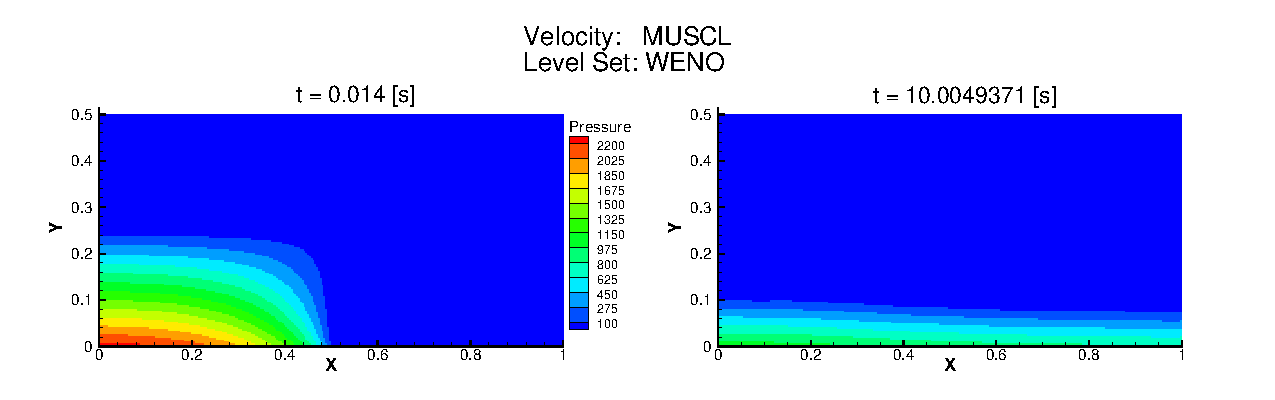
\includegraphics[width=1\textwidth]{dambreak2020_V_MUSCL_LS_WENO_Pressure.eps}
	\caption[Dambreak 2020 MUSCL - WENO Pressure field]{Pressure field at the beginning and at the end of the simulation using MUSCL to advect the velocity and WENO to advect the Level Set.}\label{dambreak2020_V_MUSCL_LS_WENO_Pressure}
\end{figure}\noindent
This combination ran without problems up to the $10$-second mark, with seemingly no loss of denser fluid. This result was obtained with the WENO smoothness indicators turned on. An earlier attempt with them deactivated diverged after a few seconds of simulation time.\par
While the previous two results show how the higher diffusivity of the MUSCL scheme helps keep in check irregularities in the Level Set field, this test shows that this is not the only factor contributing to stability. The velocities involved when using MUSCL for advecting them are lower, and this is sufficient to keep the instabilities in check, at least for up to $10$ seconds.
\subsubsection{Velocity reconstructed with MUSCL, Level-Set reconstructed with MUSCL}
\begin{figure}[!ht]
	\centering
	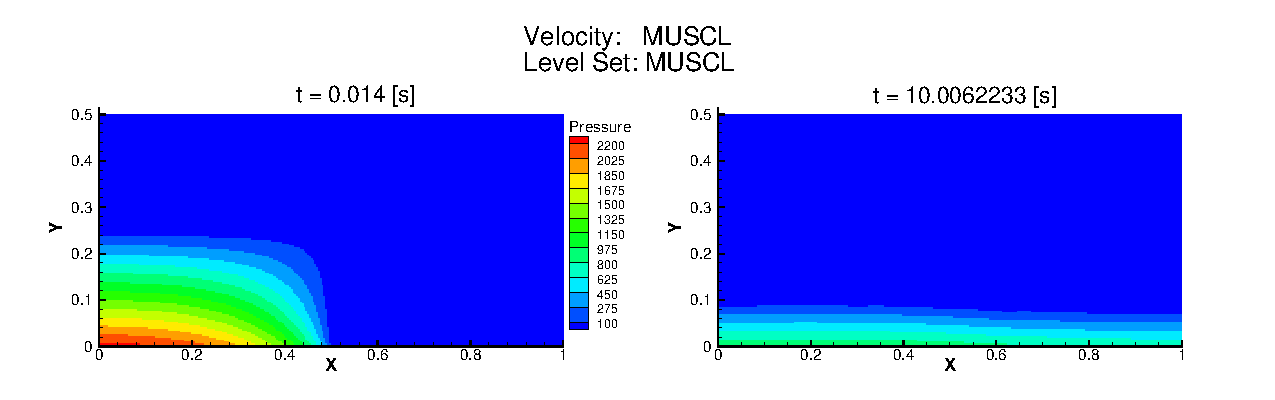
\includegraphics[width=1\textwidth]{dambreak2020_V_MUSCL_LS_MUSCL_Pressure.eps}
	\caption[Dambreak 2020 MUSCL - MUSCL Pressure field]{Pressure field at the beginning and at the end of the simulation using MUSCL to advect both the velocity and the Level Set.}\label{dambreak2020_V_MUSCL_LS_MUSCL_Pressure}
\end{figure}\noindent
This setup, again, ran smoothly for the entire $10$ seconds of simulation. Interestingly, despite the higher diffusivity of the MUSCL scheme for advecting the Level-Set, no loss of denser fluid is evident. This is likely due to the lower velocities involved. The behaviour is surprisingly similar to the test using MUSCL for the velocity and WENO for the Level Set, however, the shape of the interface between the two fluids appears more regular.
\begin{figure}[!ht]
	\centering
	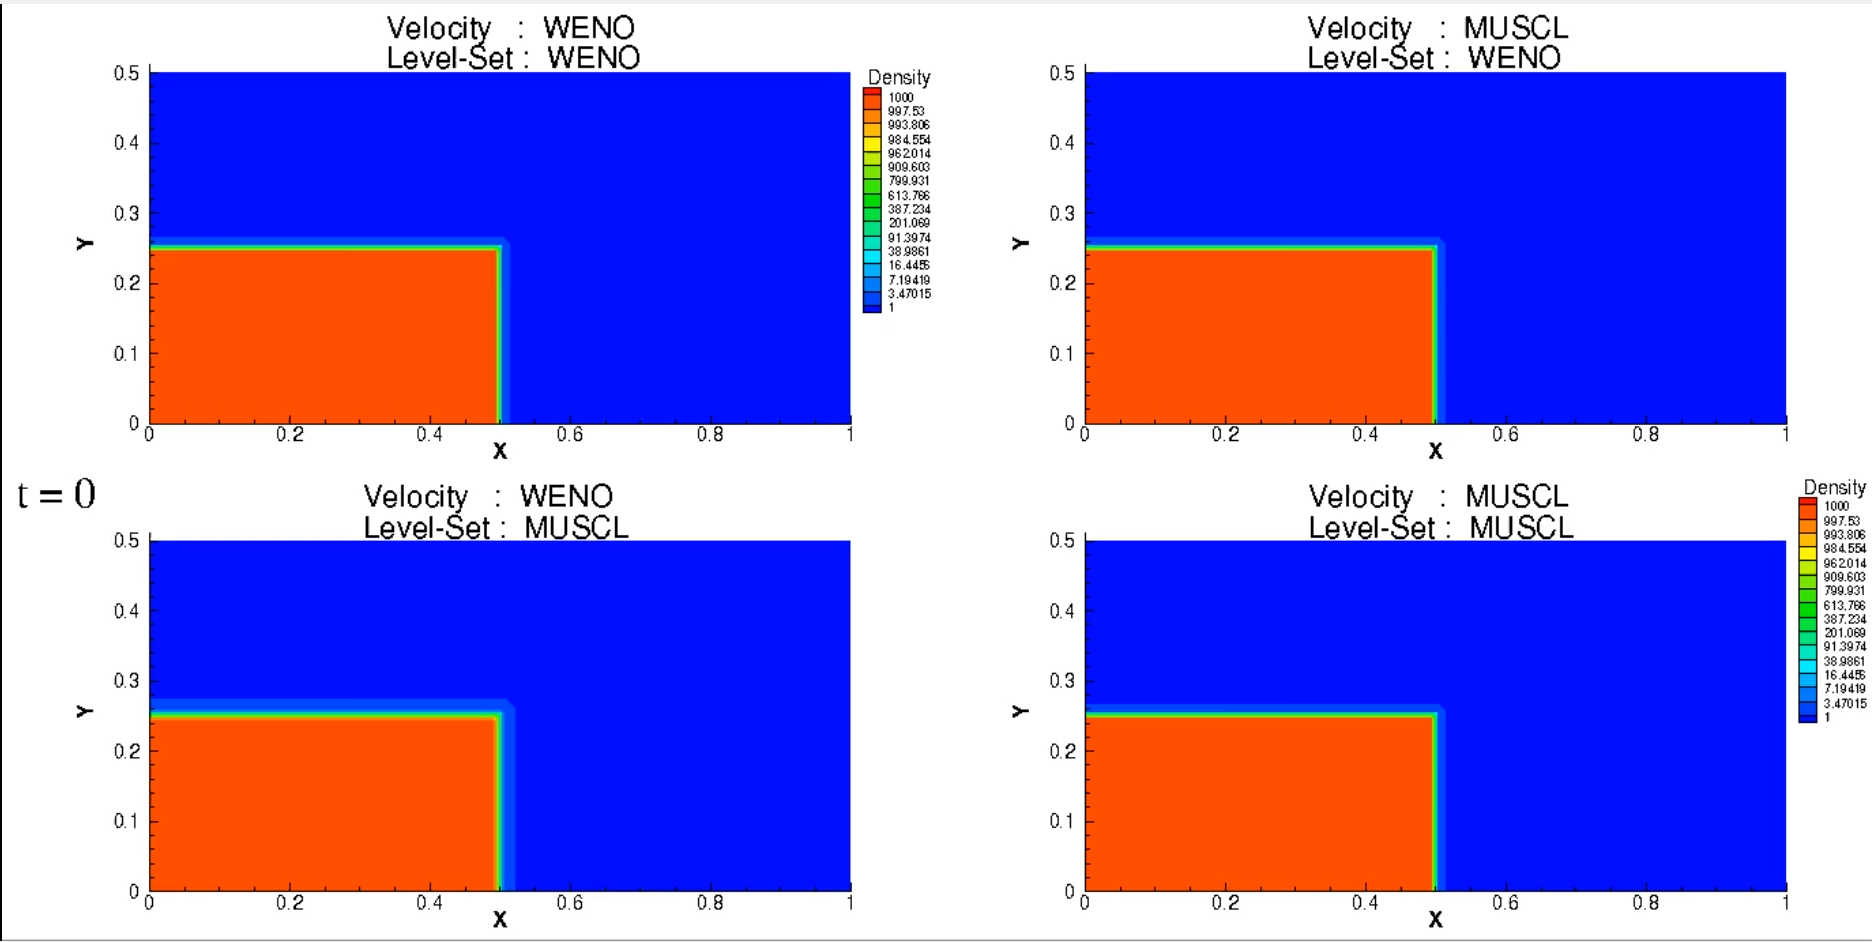
\includegraphics[width=1\textwidth]{dambreaks_t0.eps}
	\caption[Dambreak 2020 Code t=0s]{Dambreak tests in the 2020 version fo the code: $t=0\,[s]$.}\label{Dambreak4Tests_1}
\end{figure}
\begin{figure}
		\centering
		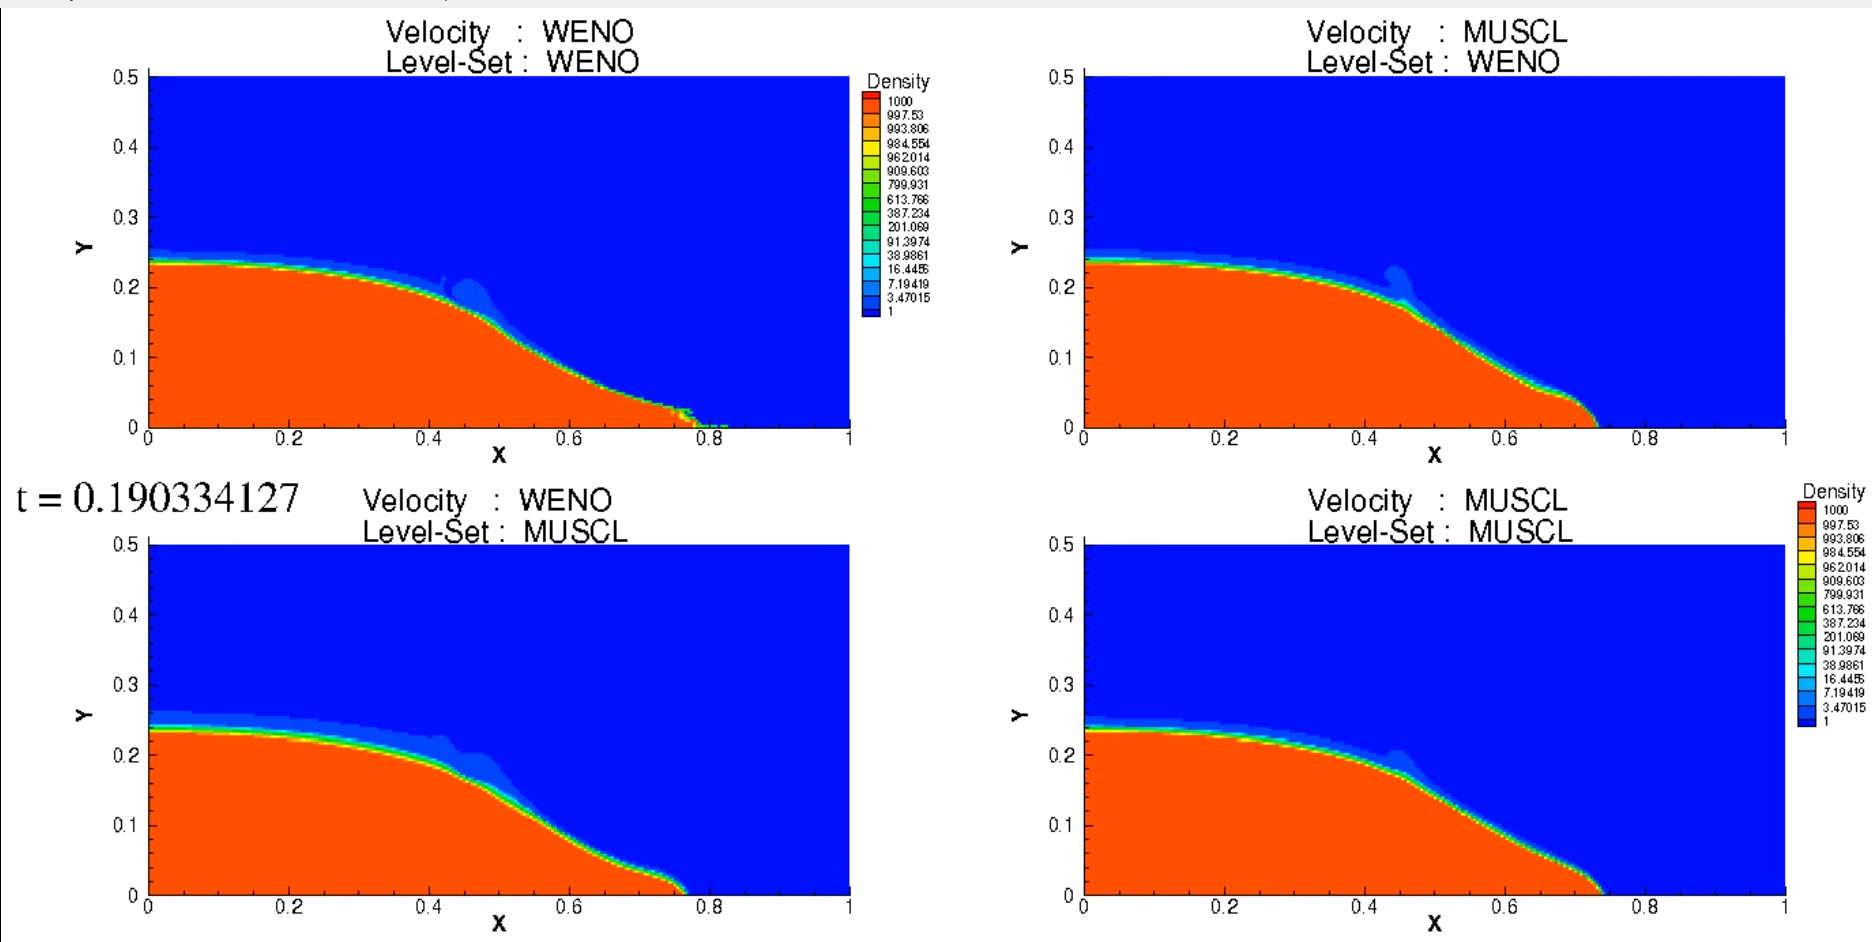
\includegraphics[width=1\textwidth]{dambreaks_t0p2.eps}
		\caption[Dambreak 2020 Code t=0.2s]{Dambreak tests in the 2020 version fo the code: $t=0.2\,[s]$.\\After, the WENO - WENO simulation diverges.}\label{Dambreak4Tests_2}
\end{figure}
\begin{figure}[!ht]
	\centering
	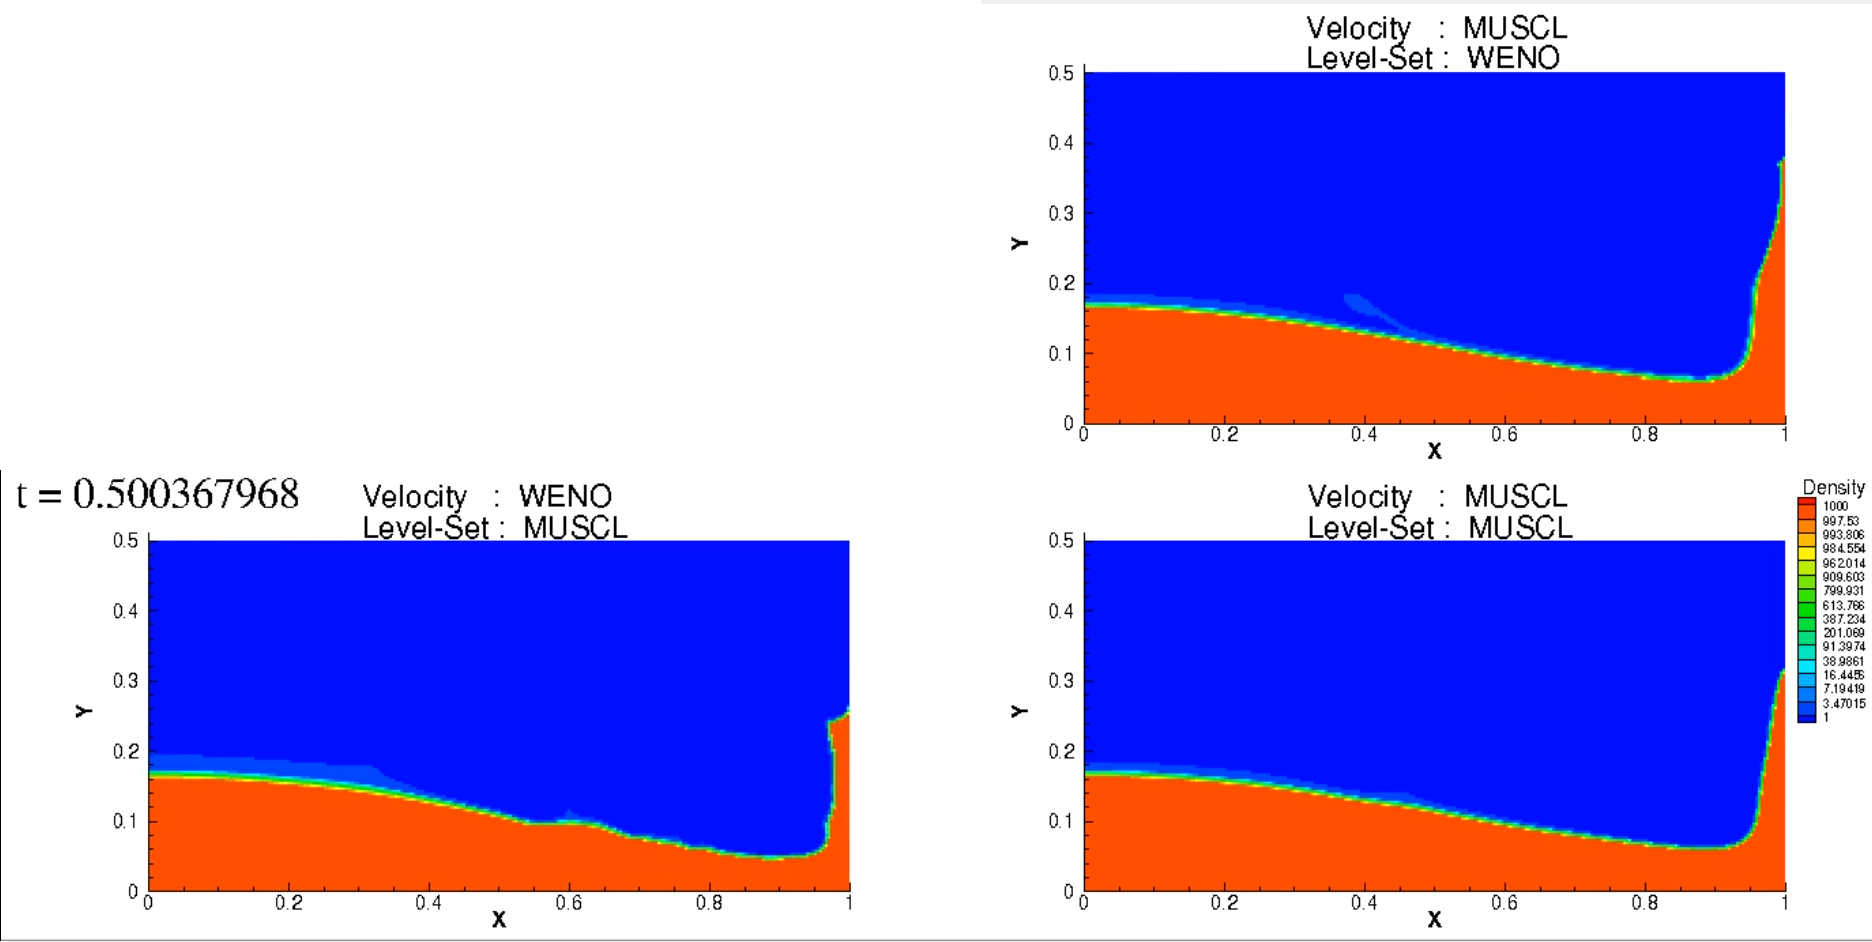
\includegraphics[width=1\textwidth]{dambreaks_t0p5.eps}
	\caption[Dambreak 2020 Code t=0.5s]{Dambreak tests in the 2020 version fo the code: $t=0.5\,[s]$.}\label{Dambreak4Tests_3}
\end{figure}
\begin{figure}[!ht]
	\centering
	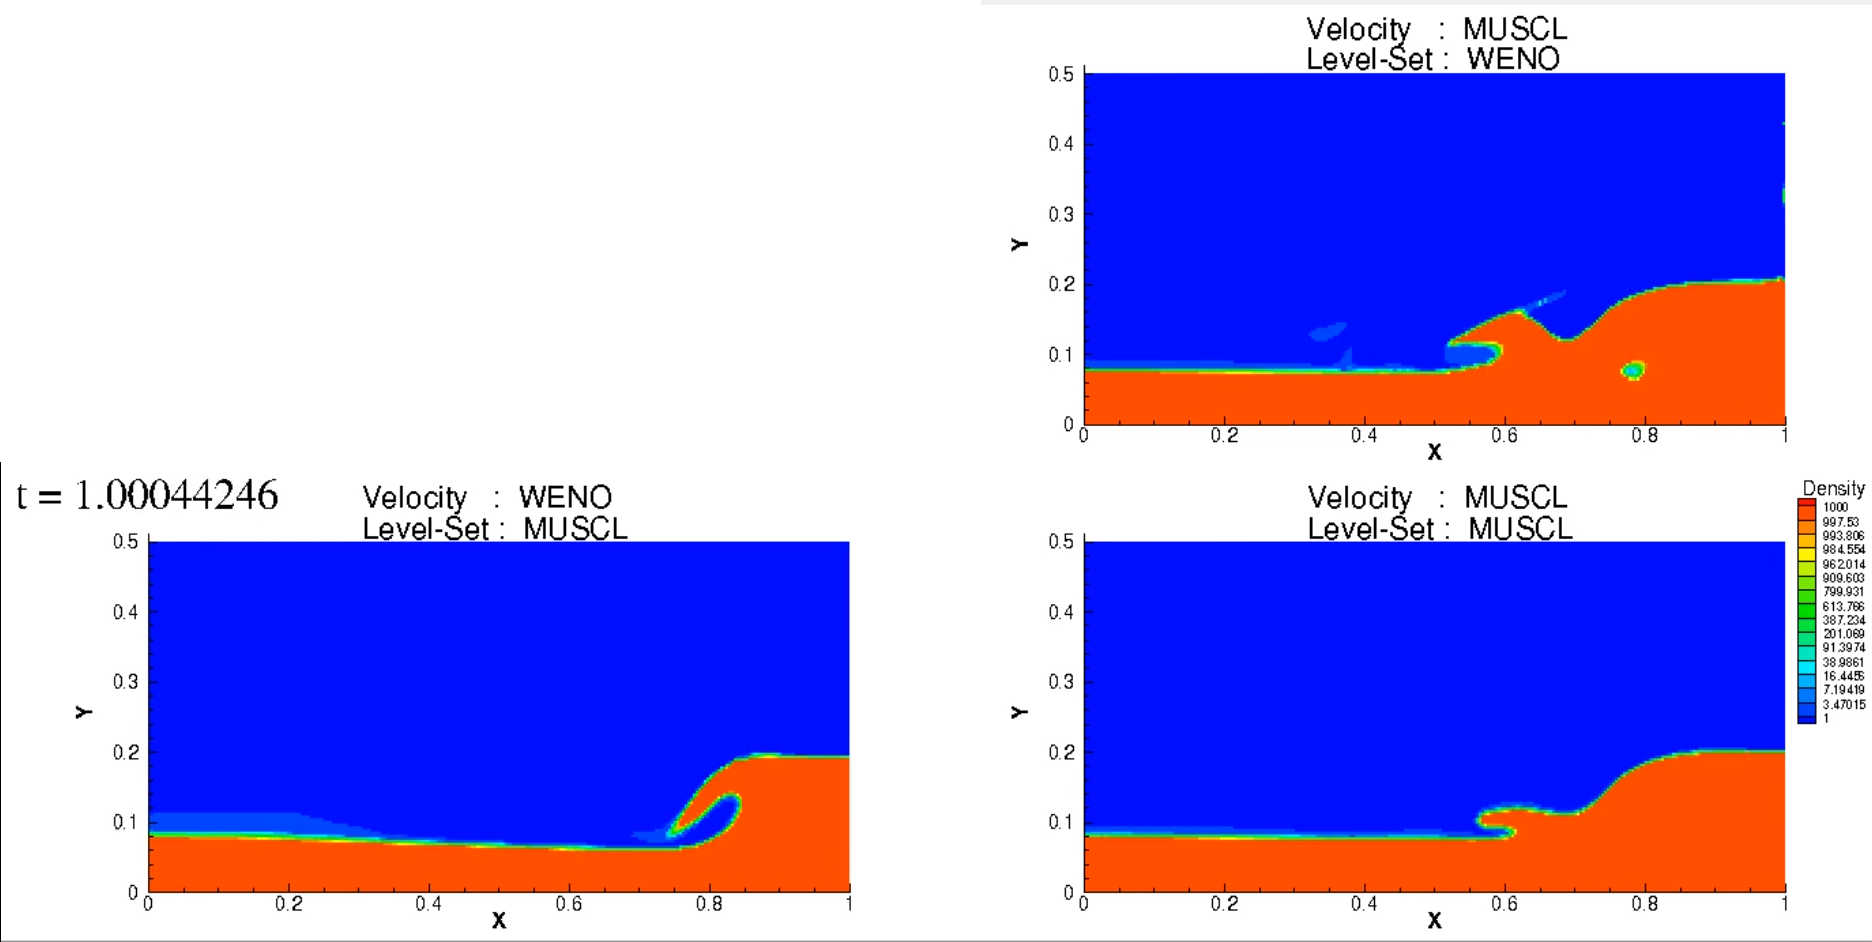
\includegraphics[width=1\textwidth]{dambreaks_t1.eps}
	\caption[Dambreak 2020 Code t=1s]{Dambreak tests in the 2020 version fo the code:$t=1\,[s]$.}\label{Dambreak4Tests_4}
\end{figure}
\begin{figure}[!ht]
	\centering
	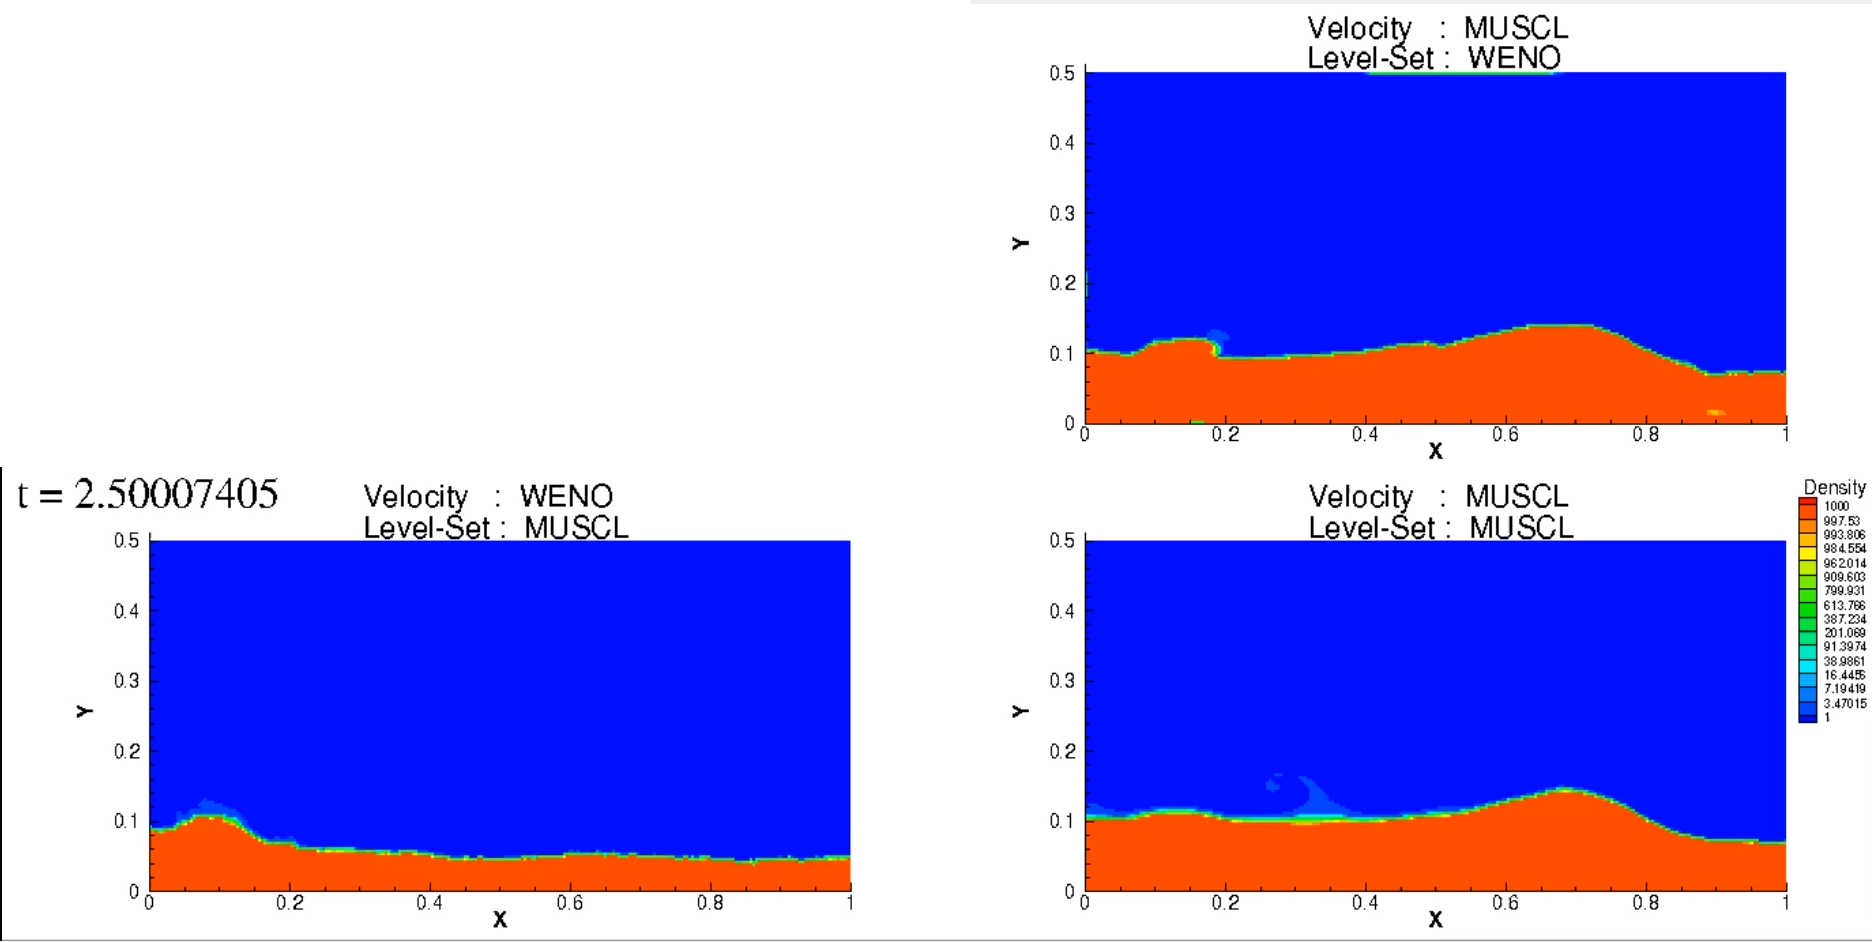
\includegraphics[width=1\textwidth]{dambreaks_t2p5.eps}
	\caption[Dambreak 2020 Code t=2.5s]{Dambreak tests in the 2020 version fo the code: $t=2.5,[s]$.}\label{Dambreak4Tests_5}
\end{figure}
\begin{figure}[!ht]
	\centering
	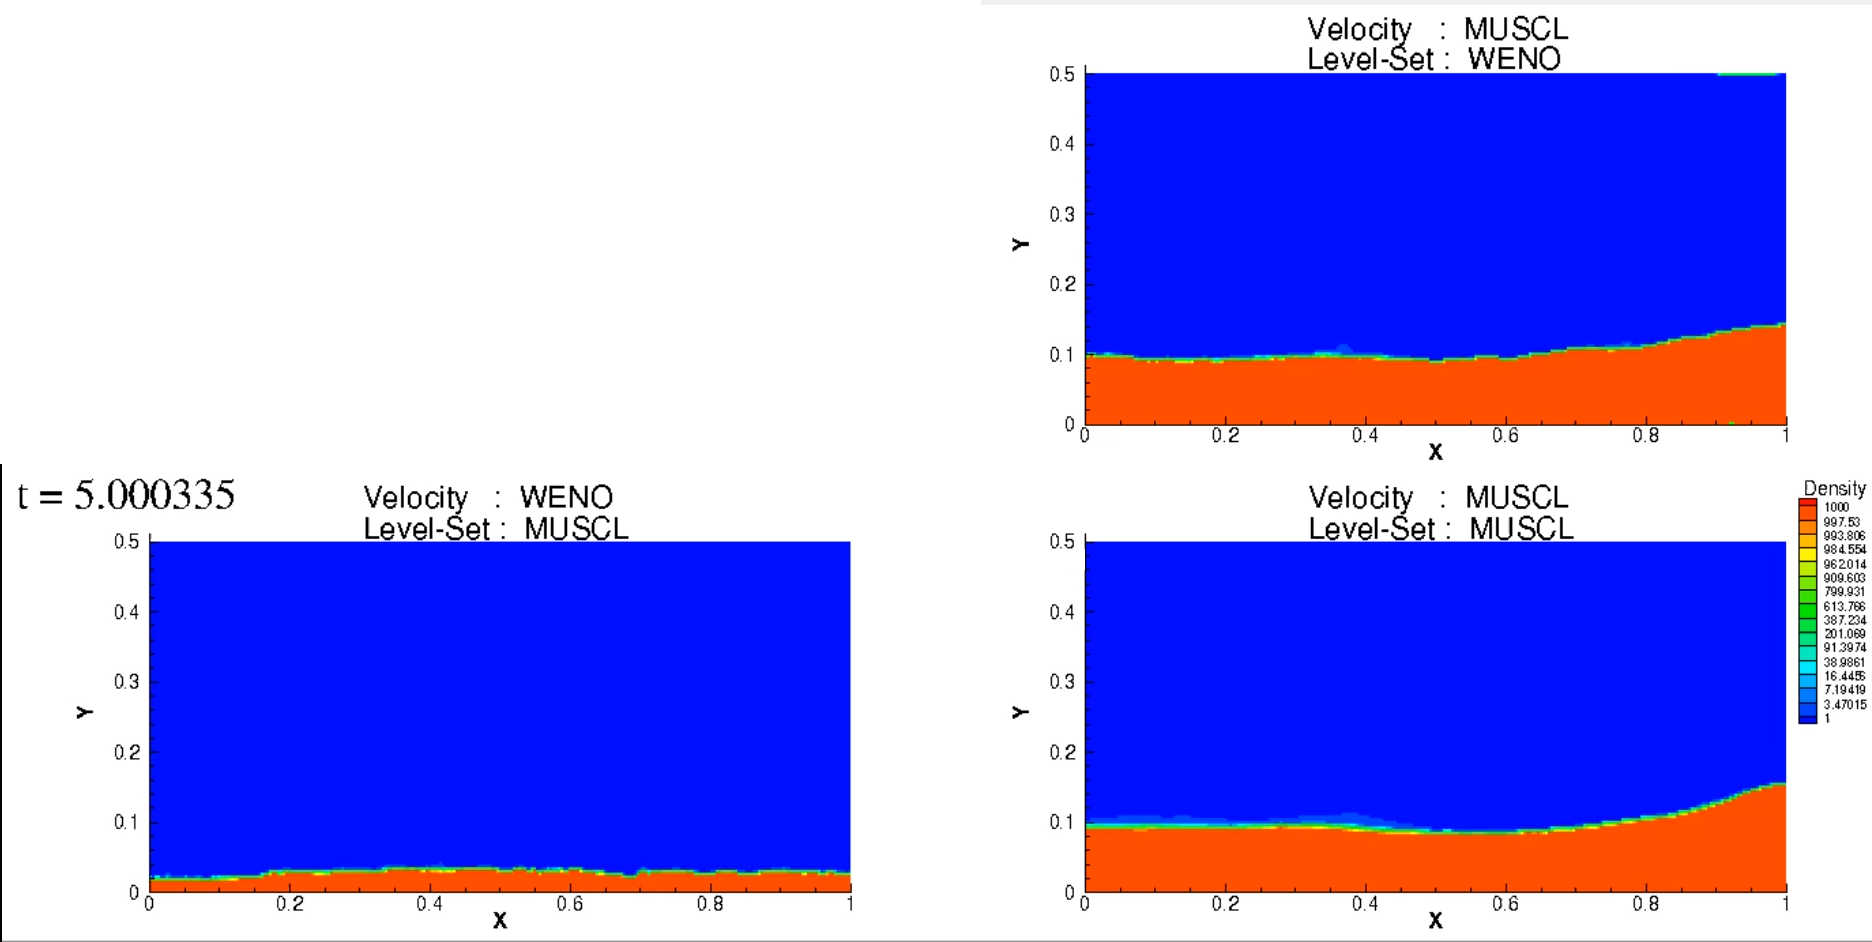
\includegraphics[width=1\textwidth]{dambreaks_t5.eps}
	\caption[Dambreak 2020 Code t=5s]{Dambreak tests in the 2020 version fo the code: $t=5\,[s]$.}\label{Dambreak4Tests_6}
\end{figure}
\begin{figure}[!ht]
	\centering
	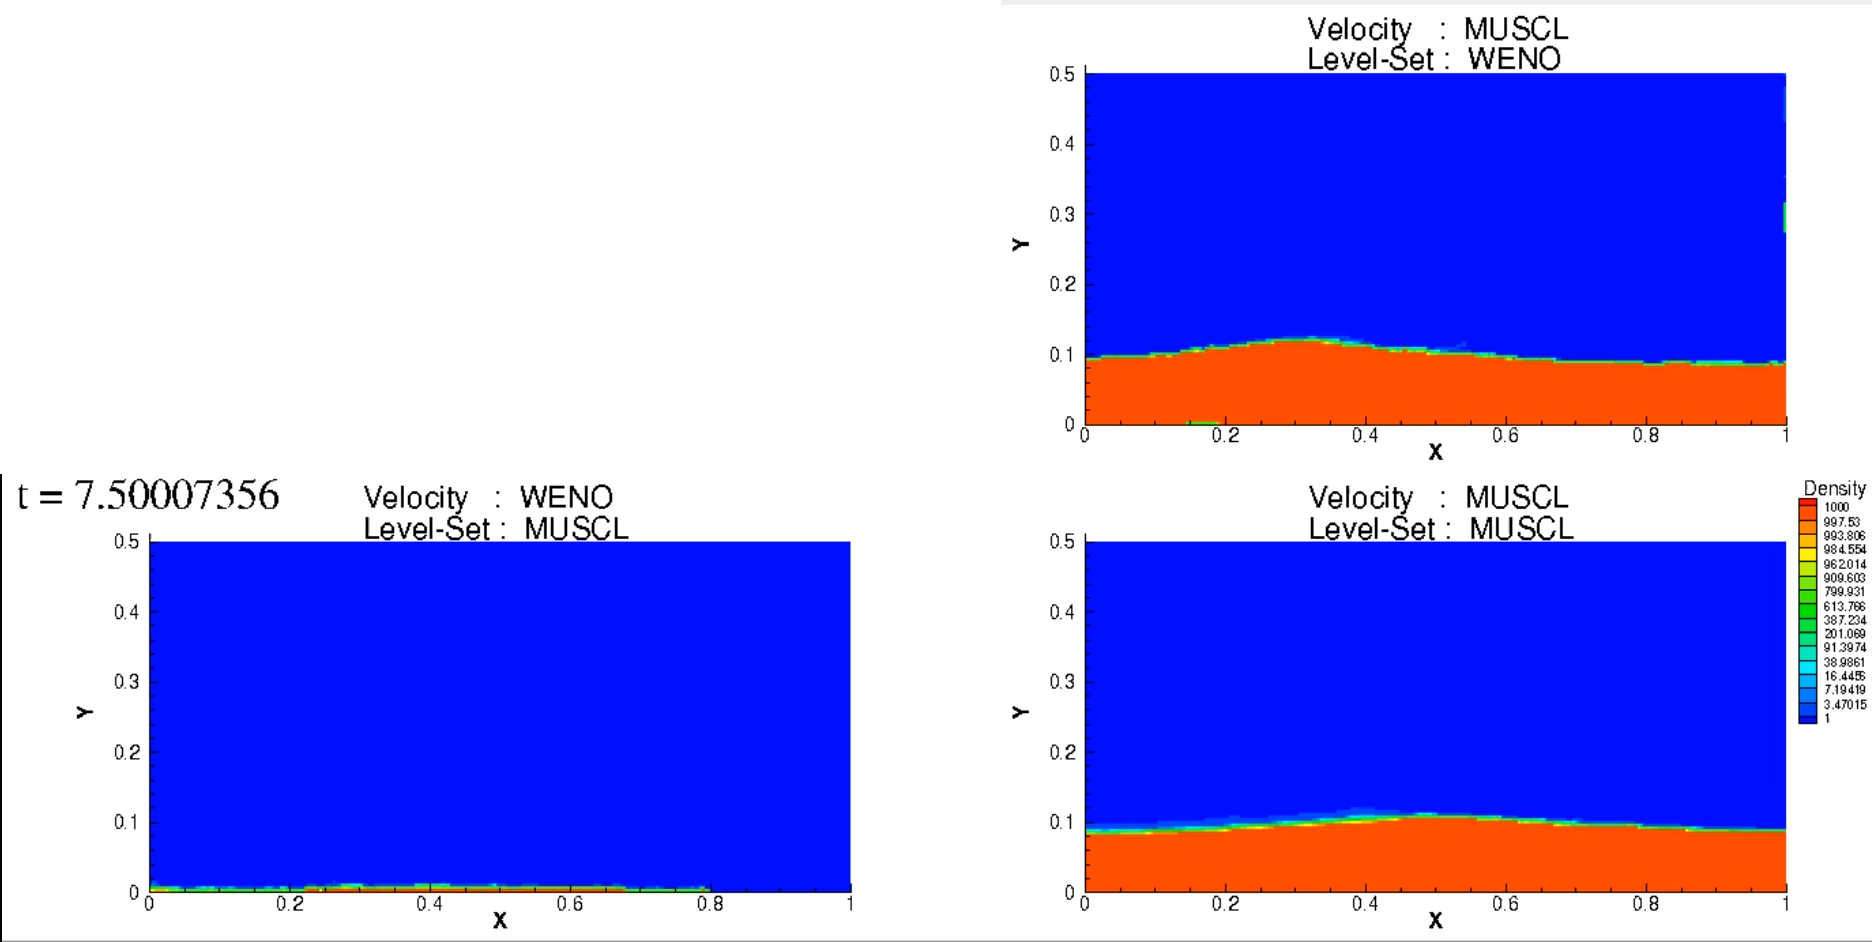
\includegraphics[width=1\textwidth]{dambreaks_t7p5.eps}
	\caption[Dambreak 2020 Code t=7.5s]{Dambreak tests in the 2020 version fo the code: $t=7.5\,[s]$.}\label{Dambreak4Tests_7}
\end{figure}
\begin{figure}[!ht]
	\centering
	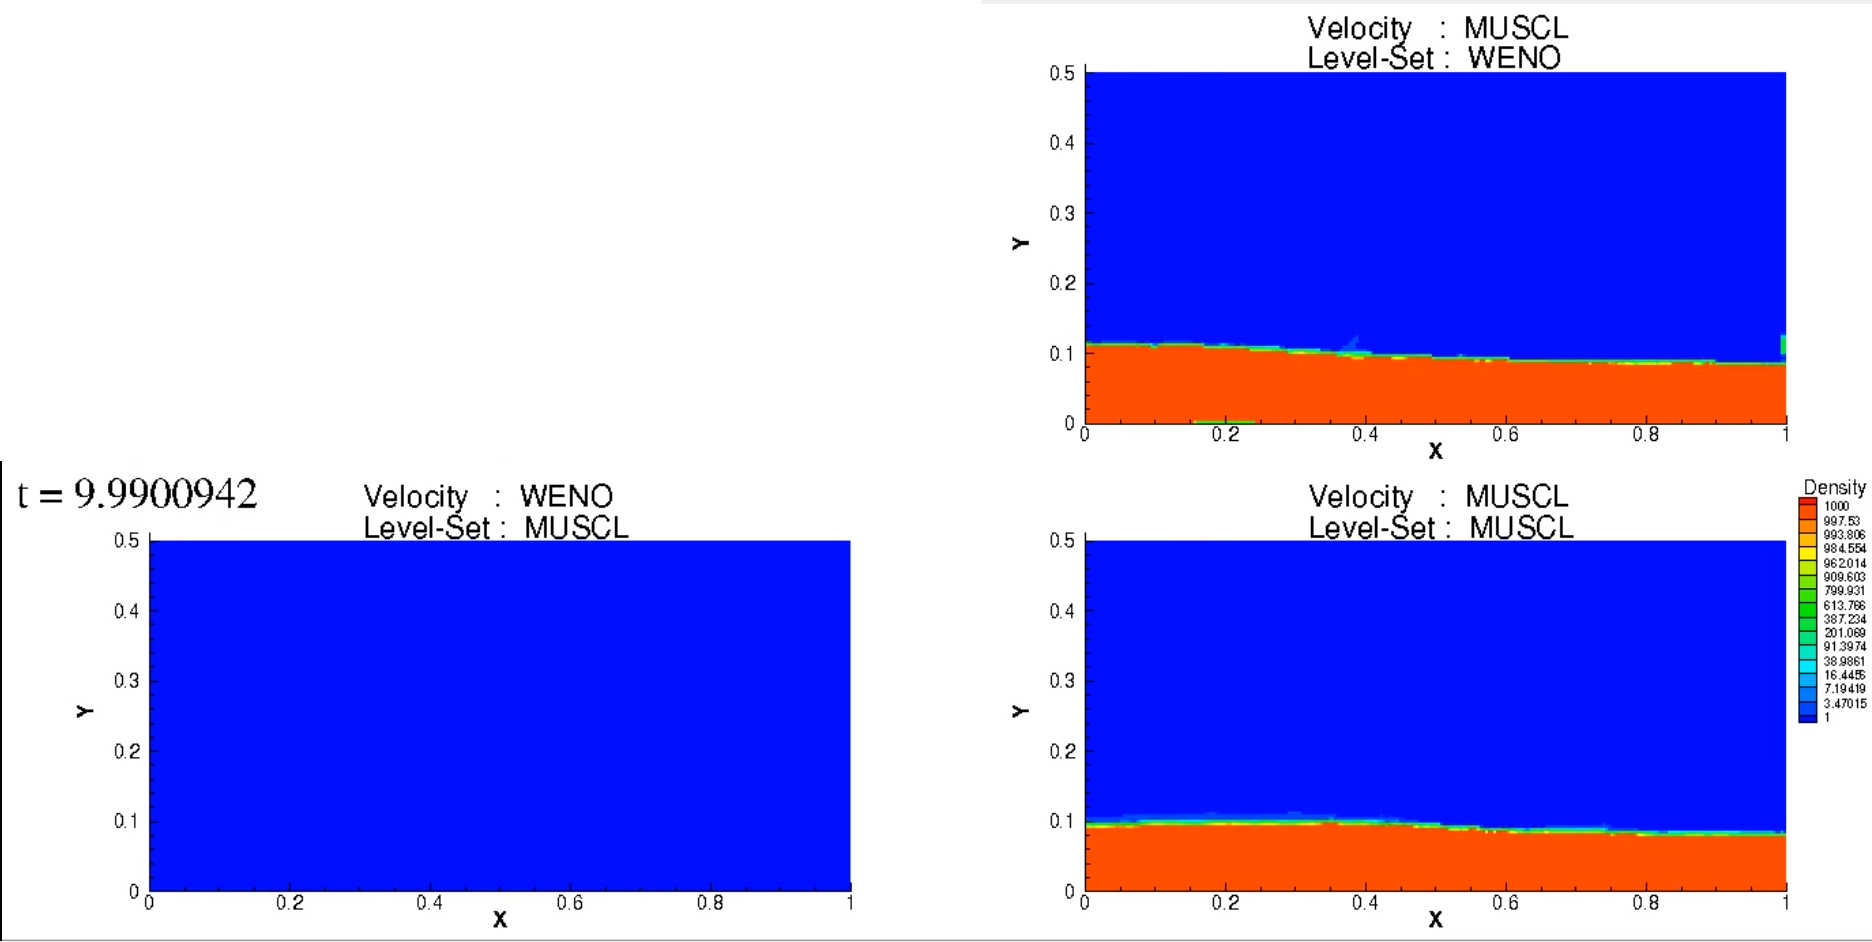
\includegraphics[width=1\textwidth]{dambreaks_t10.eps}
	\caption[Dambreak 2020 Code t=10s]{Dambreak tests in the 2020 version fo the code: $t=10\,[s]$.}\label{Dambreak4Tests_8}
\end{figure}

%----------------------------------------------- CHAPTER 6 ------------------------------------------------------------------------------------
\chapter{Conclusions}\label{Chapter_Conclusions_and_Future_Work}
The development of a multiphase method in Grid-flow is, presently, at an early stage. Some of the results are promising, but many obstacles remain.\par
At the moment, the principal difficulties are the instability of the WENO - WENO simulations and the spurious oscillations in the hydrostatic case.\par
It should be noted that, on one side, multiphase flows with high density ratios are notoriously difficult to treat and, on the other, a vast literature on multi-fluid schemes has accumulated over the last few decades.\par 
Many avenues are open to further investigate and to try to mitigate the instabilities encountered. Checks on the regularity of the density field can be implemented, modifications can be applied to the advection equation, or to the computation of the density field from the Level-Set.\par
An aspect that so far has not been explored is the redistantiation function \eqref{RedistantiationFunction}. While its use for correcting the Level Set field has been proven, in \cite{Bardin2015}, to be a source of instabilities for Grid-flow's WENO scheme, it could be used to regularize it when computing the density.\par
The ghost fluid method, as an alternative to the delta functions used so far, can be explored.\par
Once the stability problems are tackled, the mass conservation properties of the scheme should be investigated, as they are known to be a critical point for the Level Set method. If these are deemed insufficient, many improvements to the base method can be explored, such as coupling with a volume of fluid method, coupling with a Lagrangian method and so on.\par
Other aspects that were ignored and that warrant further exploration are the inclusion of variable viscosity and surface tension.\par
Once these basic aspects are taken care of, more advanced ones, such as the coupling of the method with the immersed boundary and with the turbulence model can be dealt with.\par
These other aspects of Grid-flow are themselves currently under development, and their exploration and expansion can be, in the future, another aspect of this work.

\backmatter
\addcontentsline{toc}{chapter}{Bibliography}
\bibliographystyle{plain}
\nocite{*}
\bibliography{biblio}
\end{document}


